%!TEX root = ../AliStrangeJets.tex

\section{Results and discussion}%
\label{sec:Results}

\subsection{Particles $\pT$-differential density}
\label{subsec:ParPtDensity}

For the strange hadrons discussed in this paper, the ratios of yields for particles and anti-particles are around one within the uncertainties, as expected at these collision energies in the mid-rapidity region.
Therefore, all the $\pT$-differential density shown in the following are reported after summing particles and anti-particles.
The different selections shown in the following have been introduced in section~\ref{sec:ParJetMatch}, inwhich also introduced the normalization method. 

The $\pT$-differential density ($\dd \rho/ \dd \pT$ defined by Eq.~\ref{eq:normalize}), for all particle species, in \pp and MB \pPb collisions are shown in Fig.~\ref{fig:ppSpect} and \ref{fig:pPbSpect}, respectively.
All the hadrons' densities with $\pT$ are observed to become harder within events which require of at least one charged particle jet with $\pTjch > 10$~\GeVc.
Also, as expected the particle $\pT$-differential density in jet is harder than that in underlying events.

\begin{figure}[!ht]
	\begin{center}
		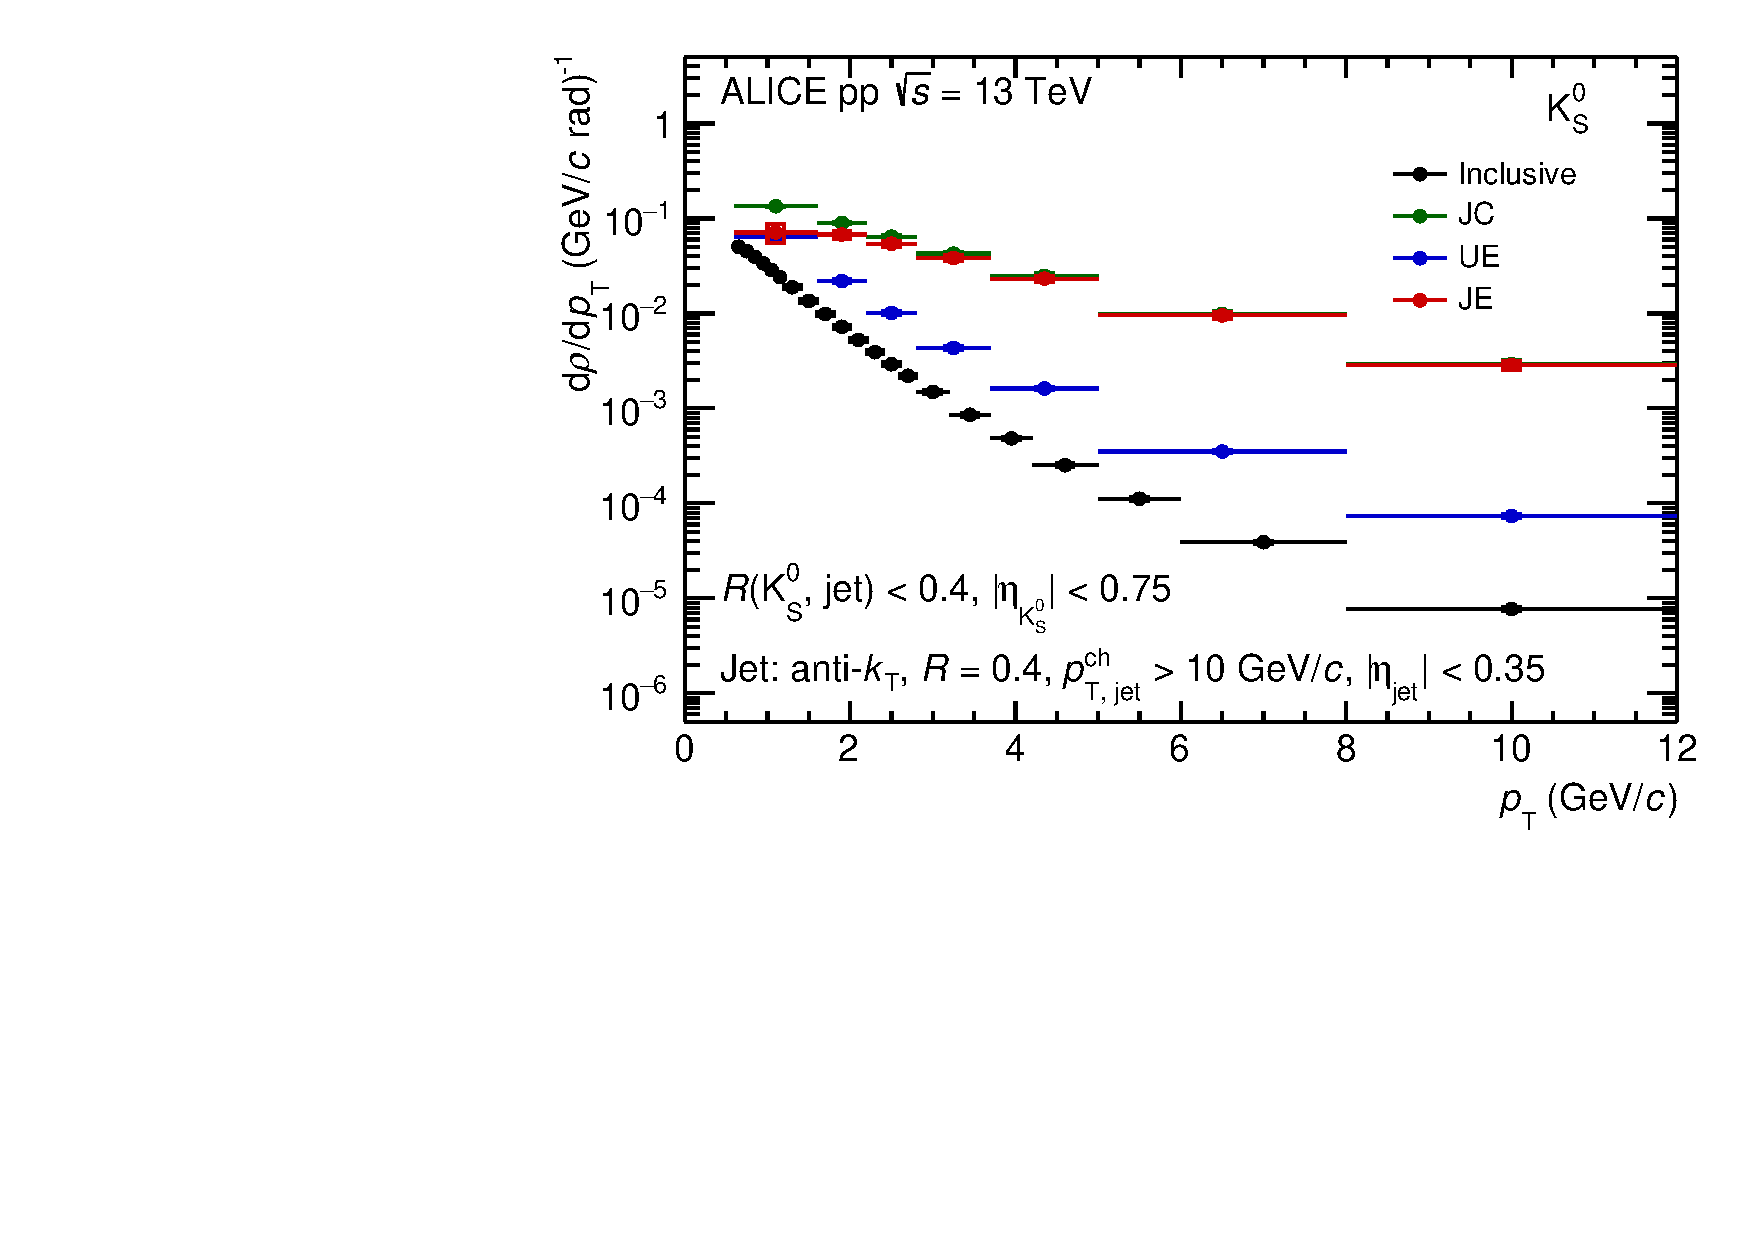
\includegraphics[width=.4\textwidth]{cf4_1}
		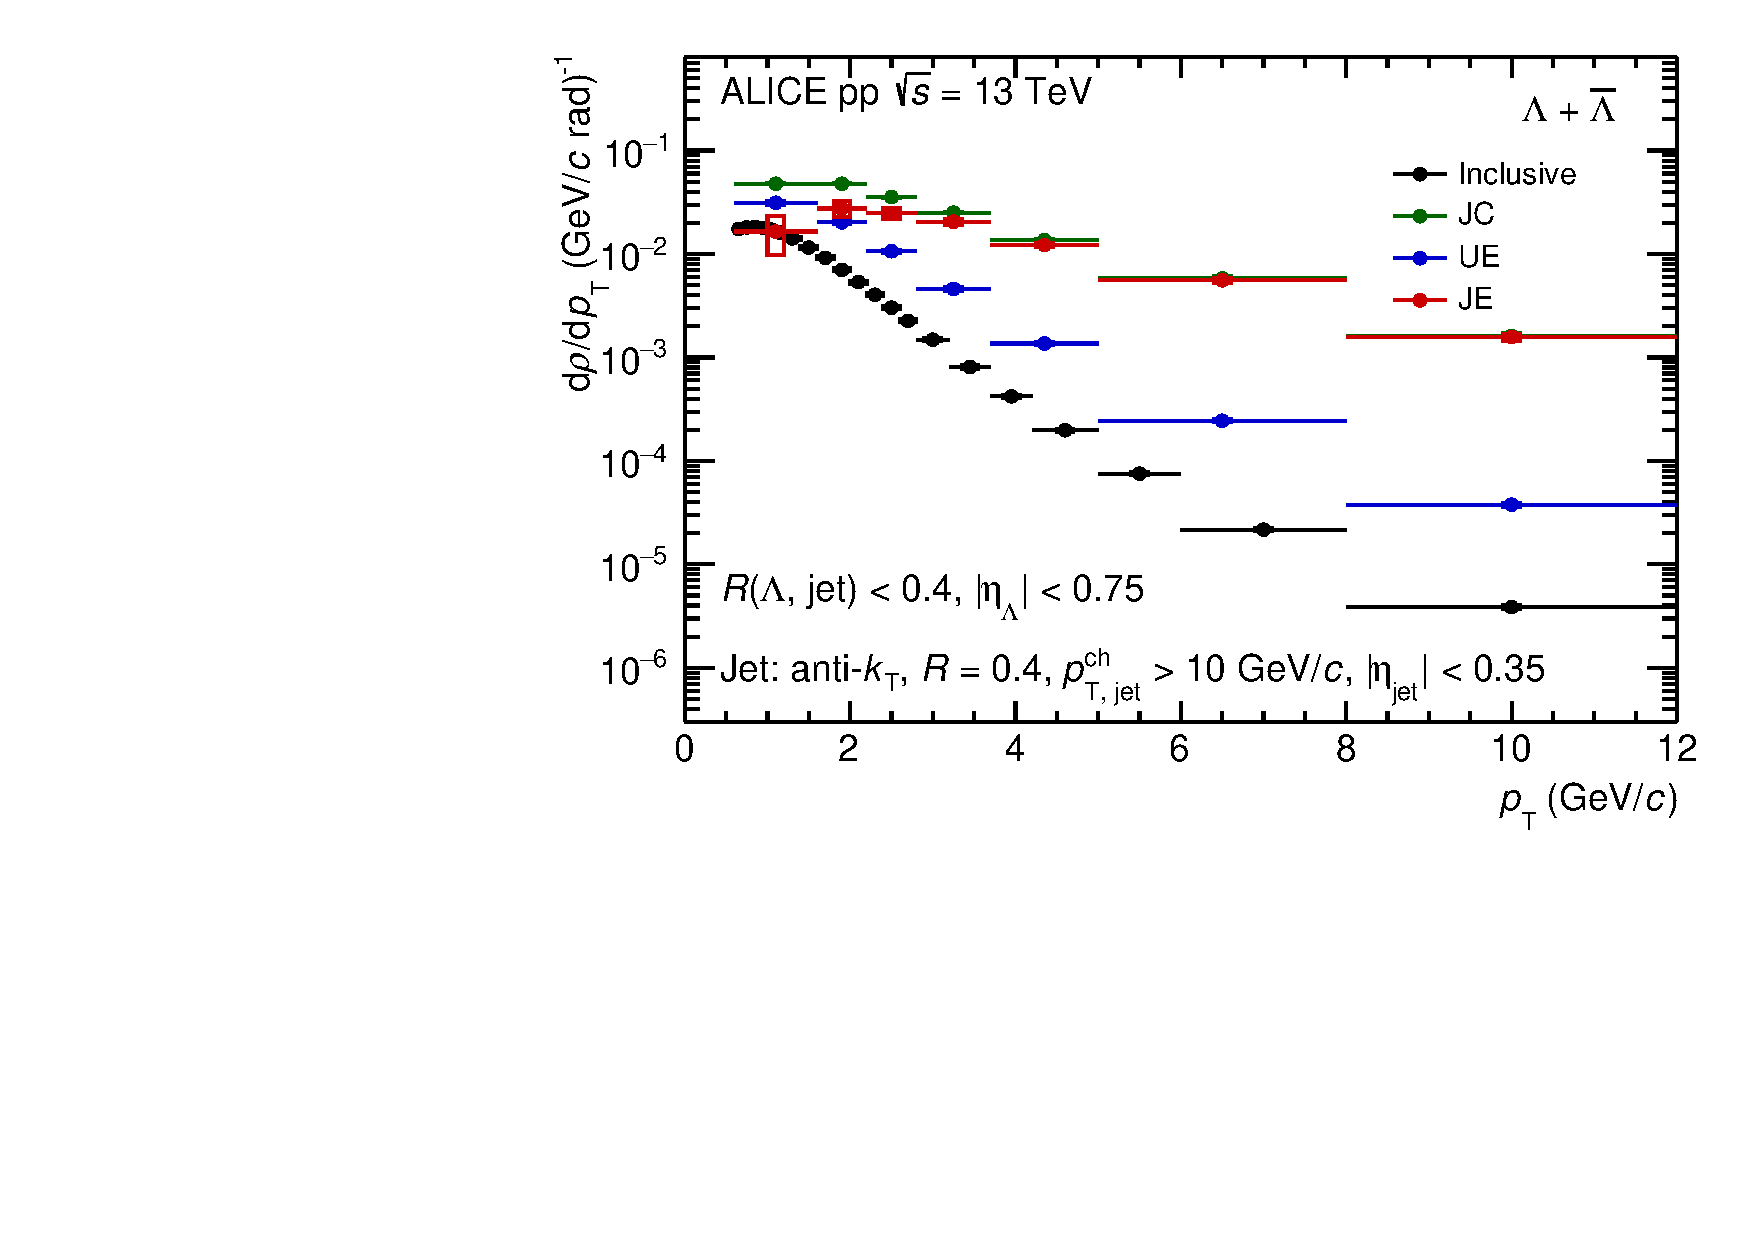
\includegraphics[width=.4\textwidth]{cf4_2}
		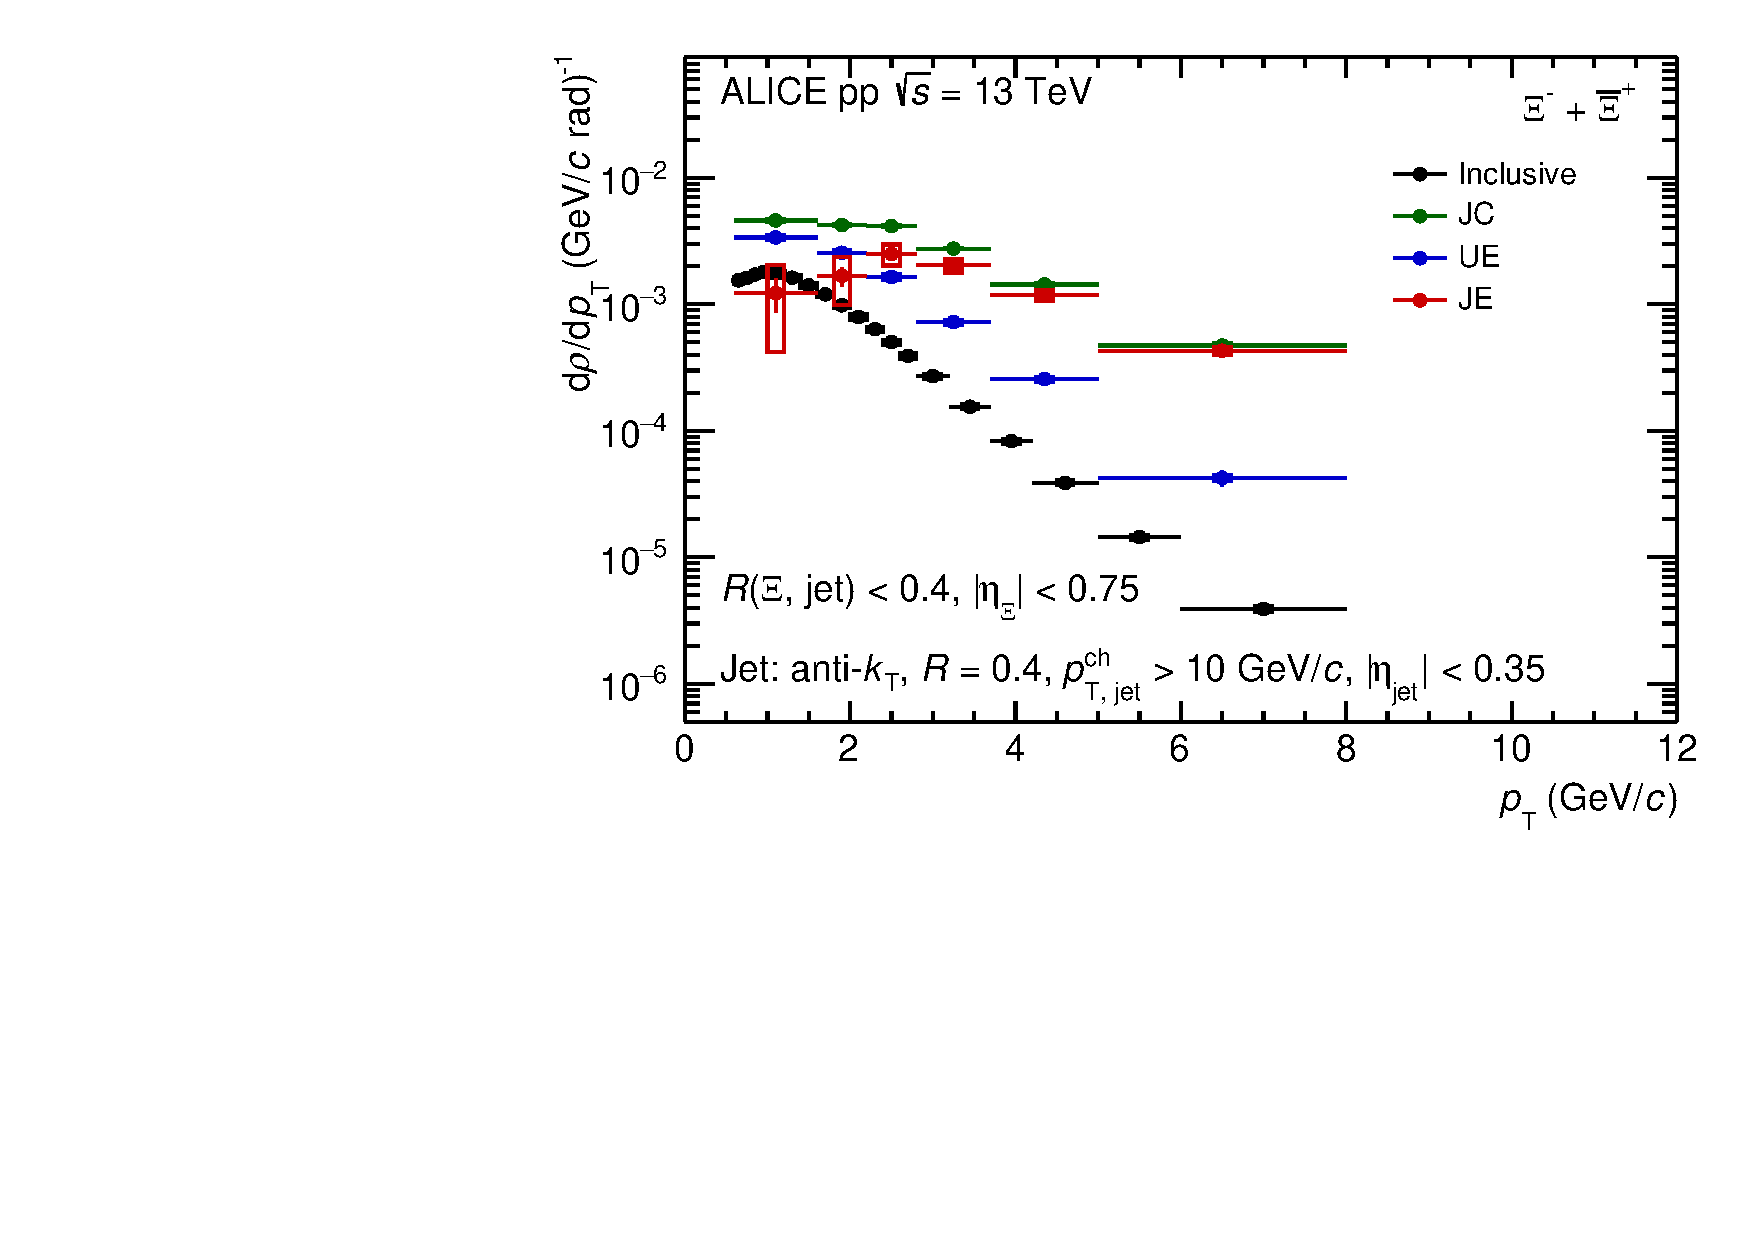
\includegraphics[width=.4\textwidth]{cf4_3}
		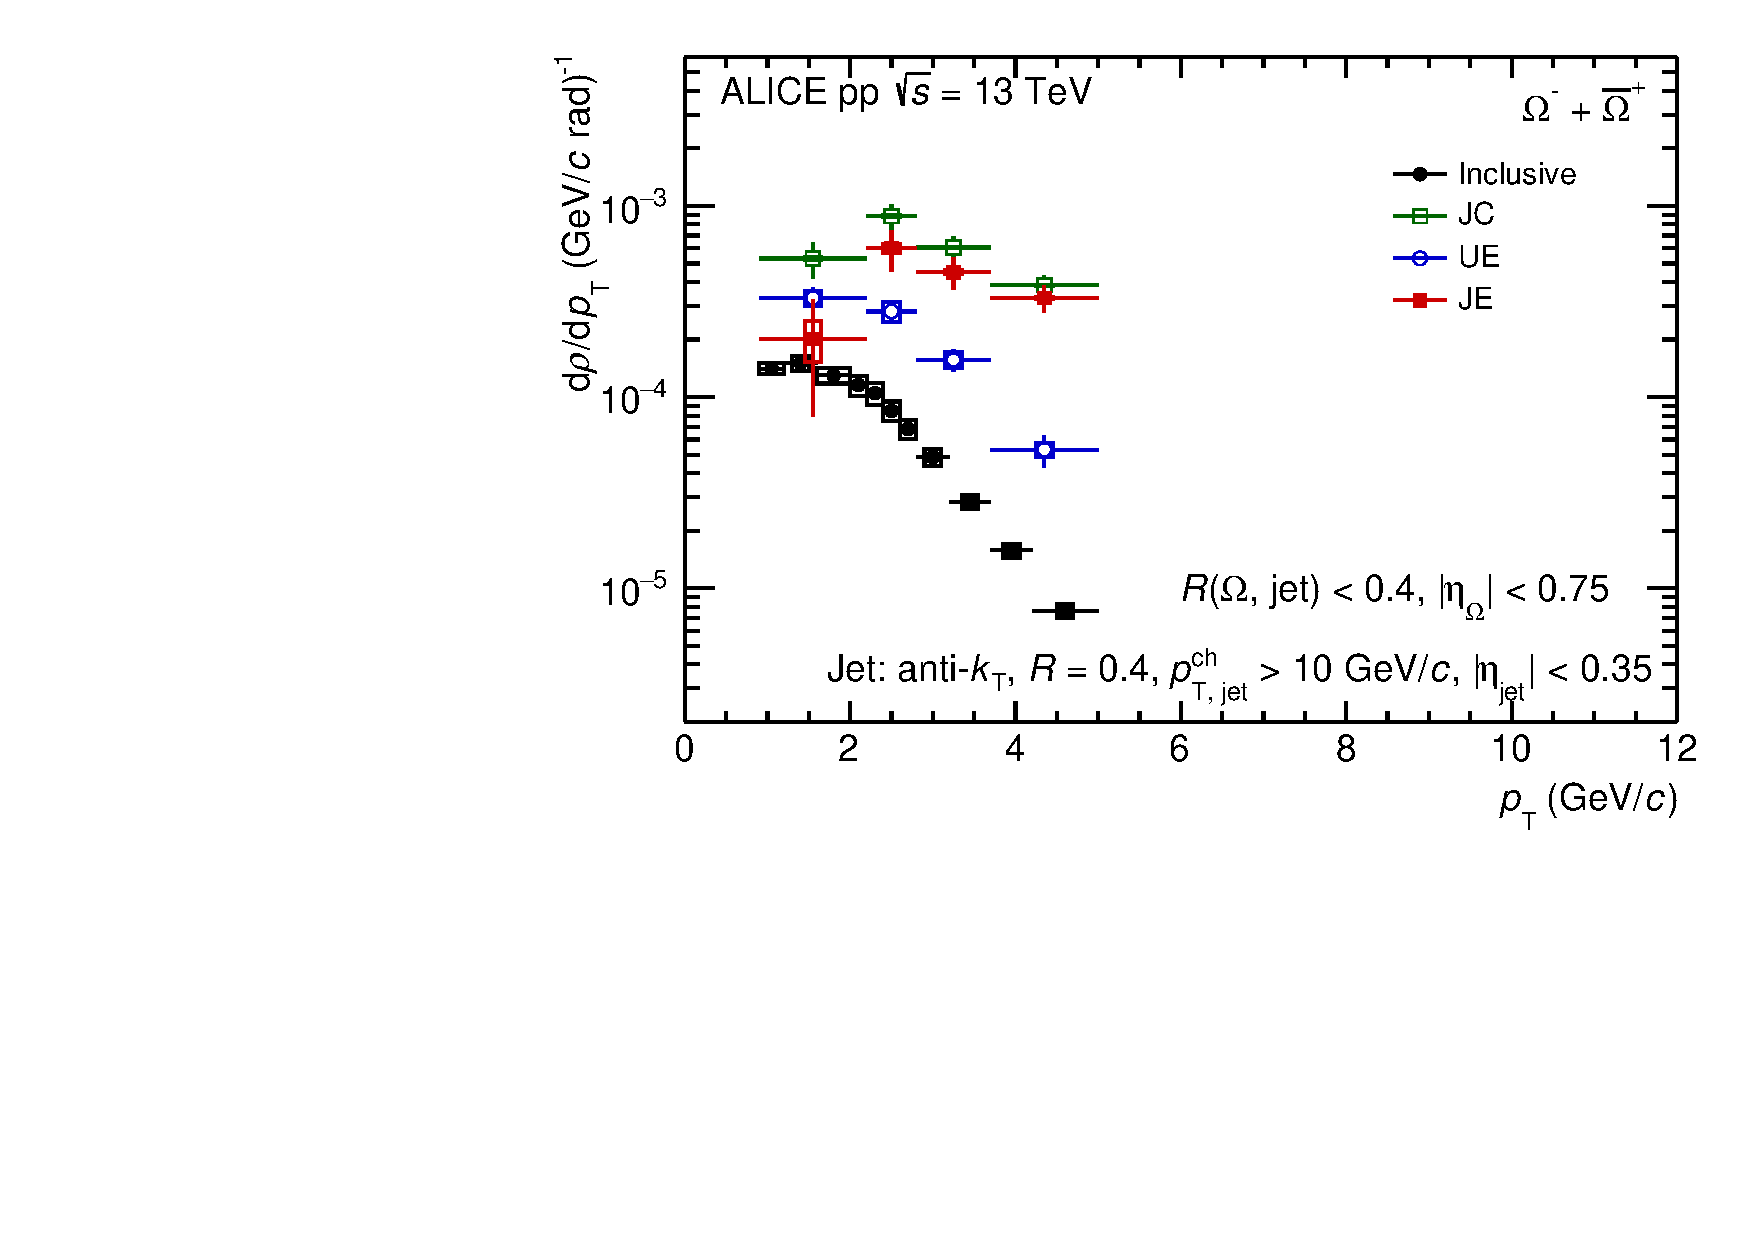
\includegraphics[width=.4\textwidth]{cf4_4}
	\end{center}
	\caption{$\pT$-differential density of $\kzero$, $\lmb + \almb$, $\X + \Ix$ and $\Om + \Mo$ in \pp at \thirteen. In those plots, the black point represent particles witch from minimum bias events, the green point represent particles which from the jet cones, the blue point represent particles within perpendicular cone of jet which associated with the underlying event and the red point represent the particle from the jet fragmentation.}
	\label{fig:ppSpect}
\end{figure}
\begin{figure}[!ht]
	\begin{center}
		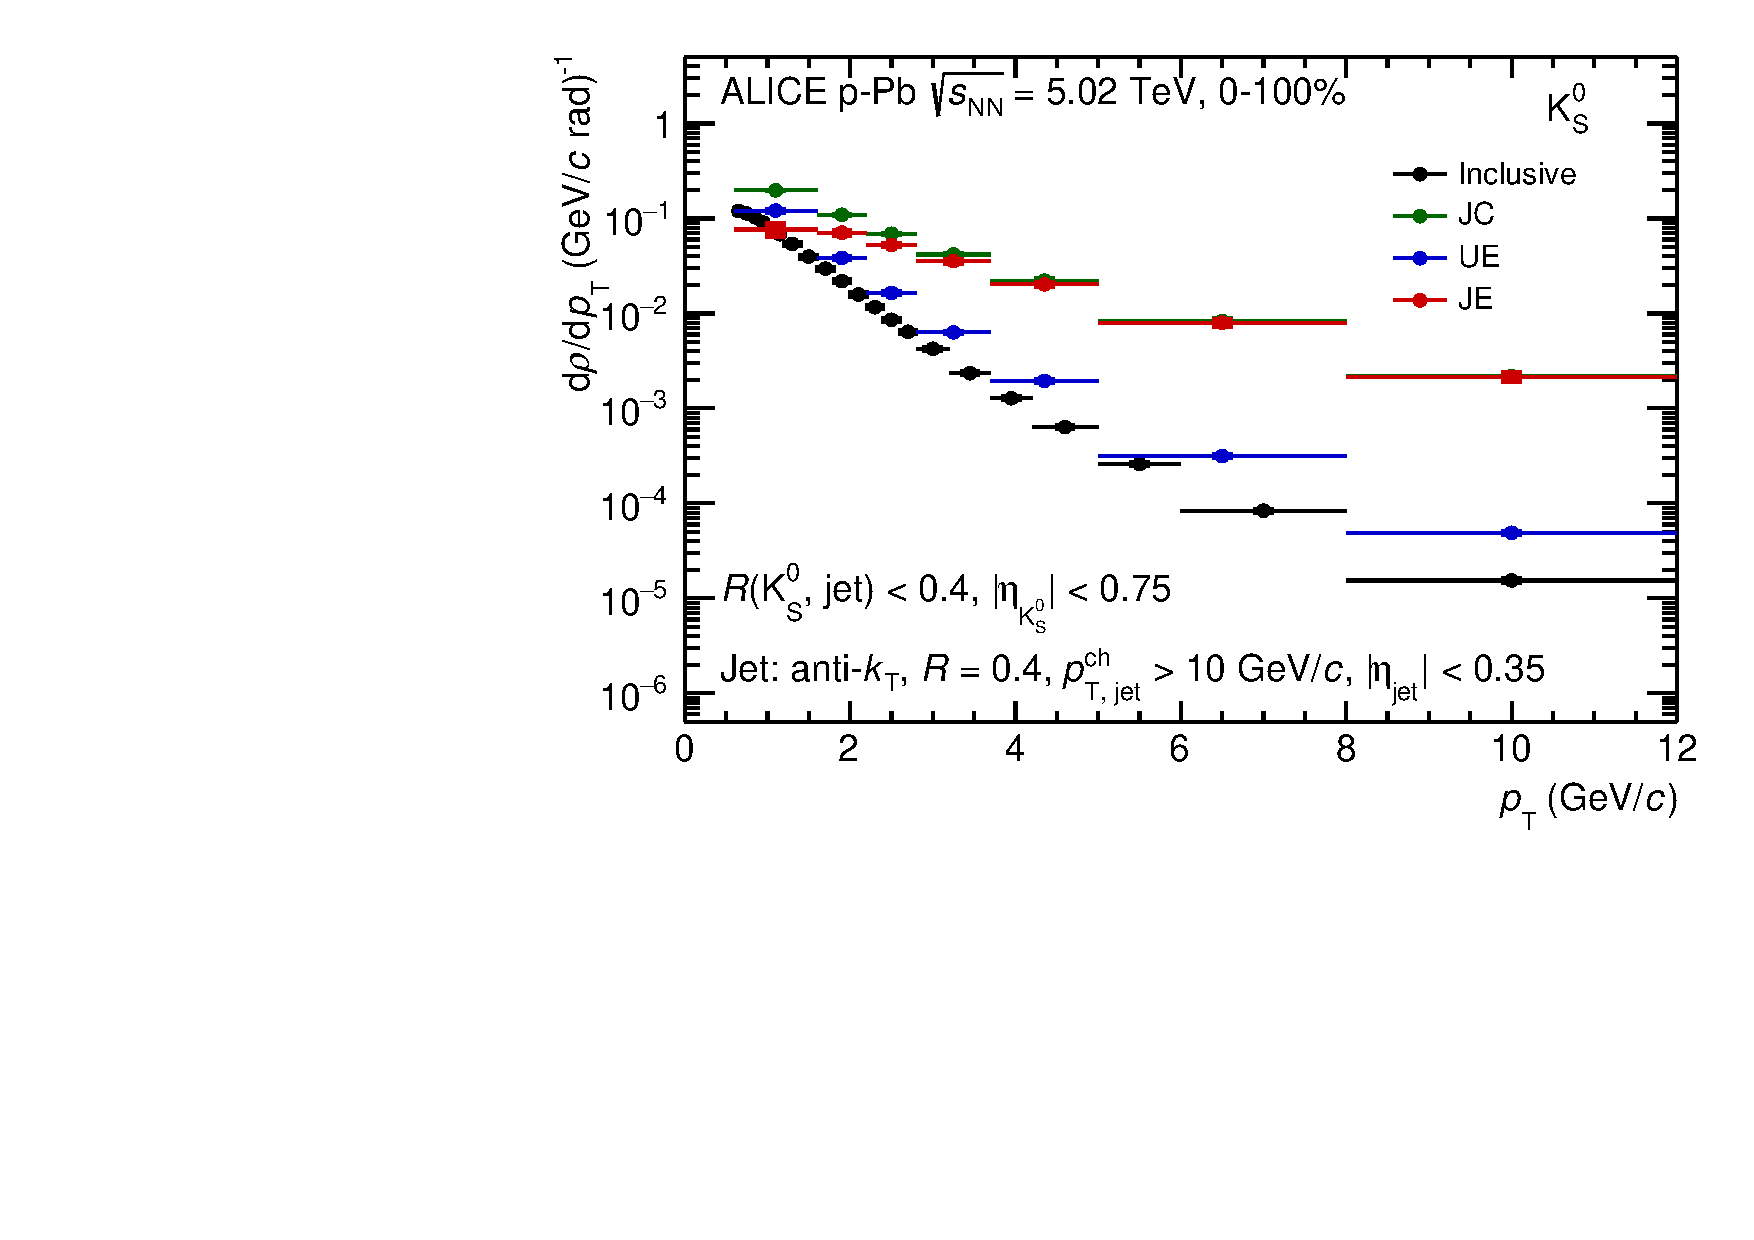
\includegraphics[width=.4\textwidth]{cf5_1}
		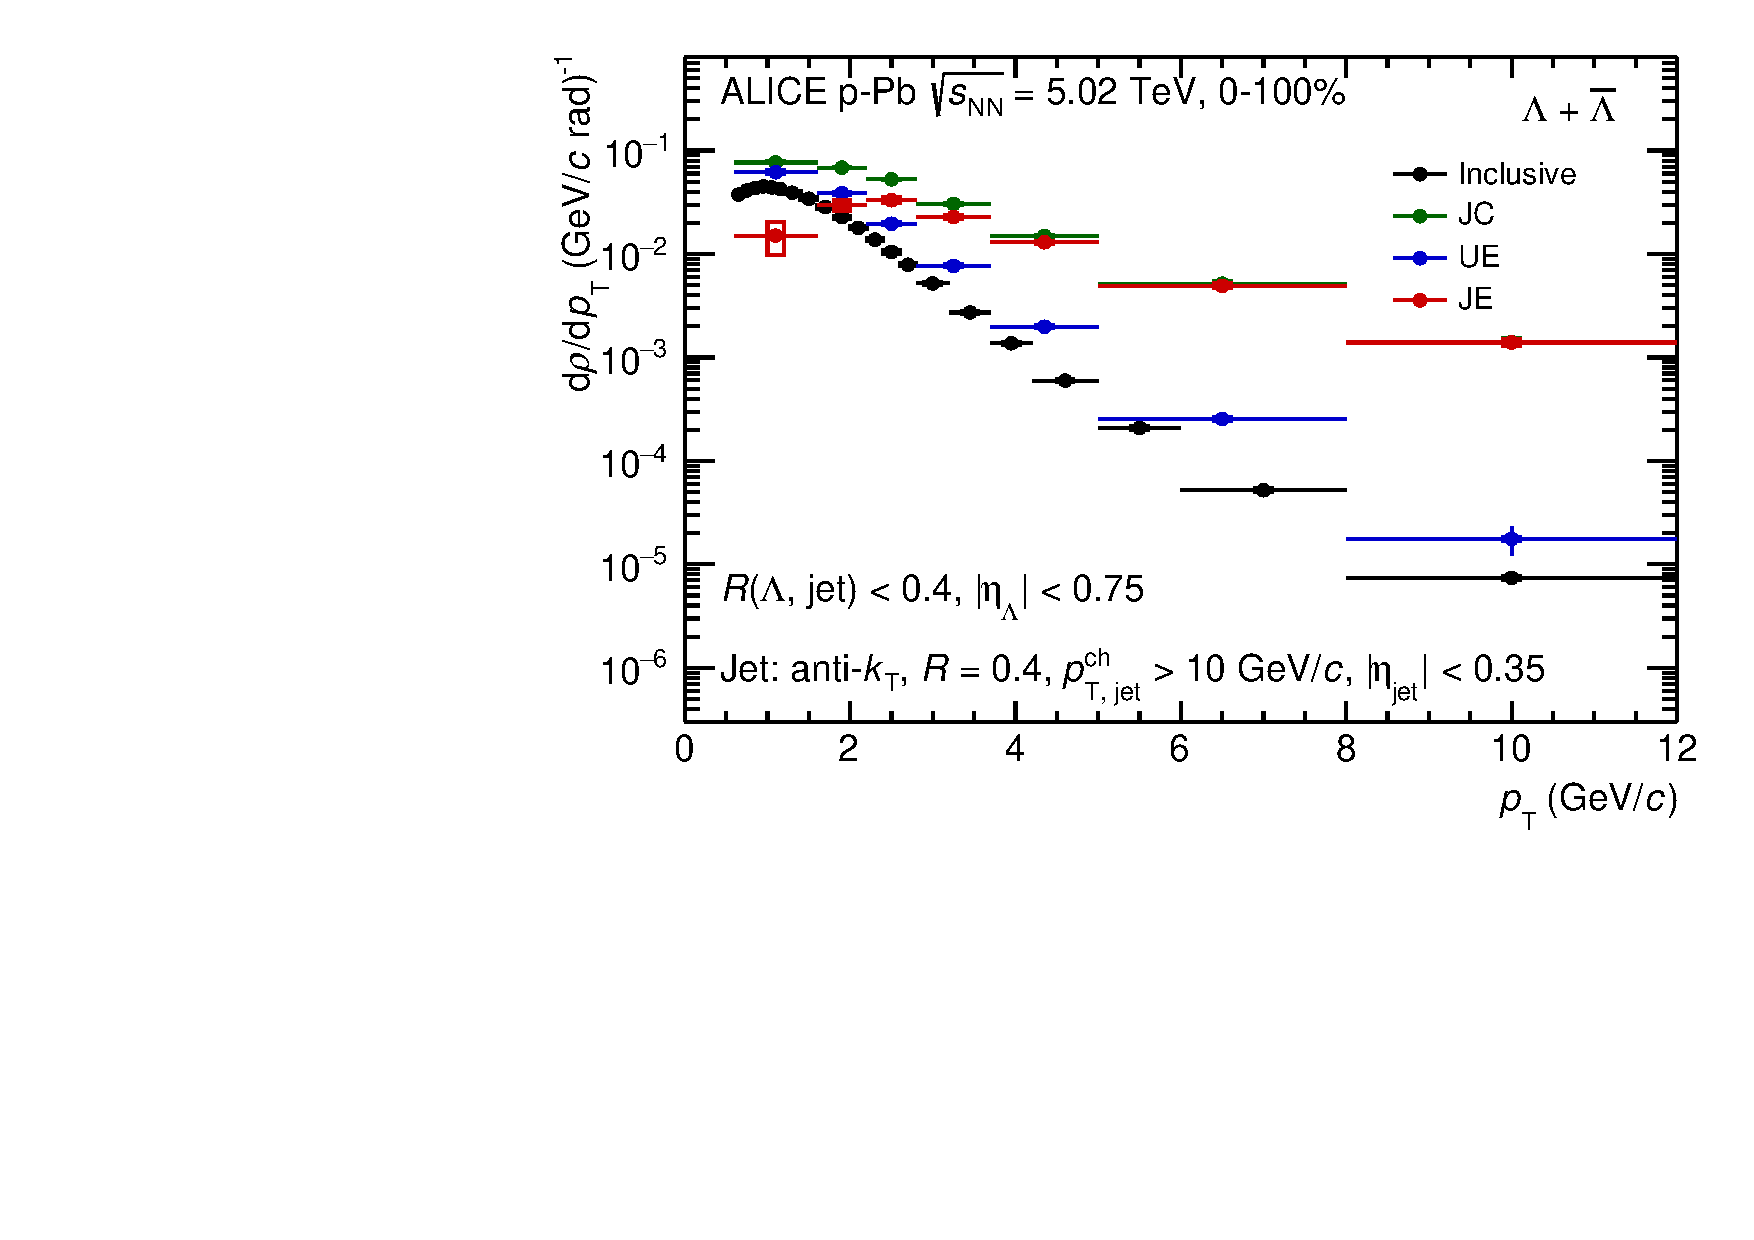
\includegraphics[width=.4\textwidth]{cf5_2}
		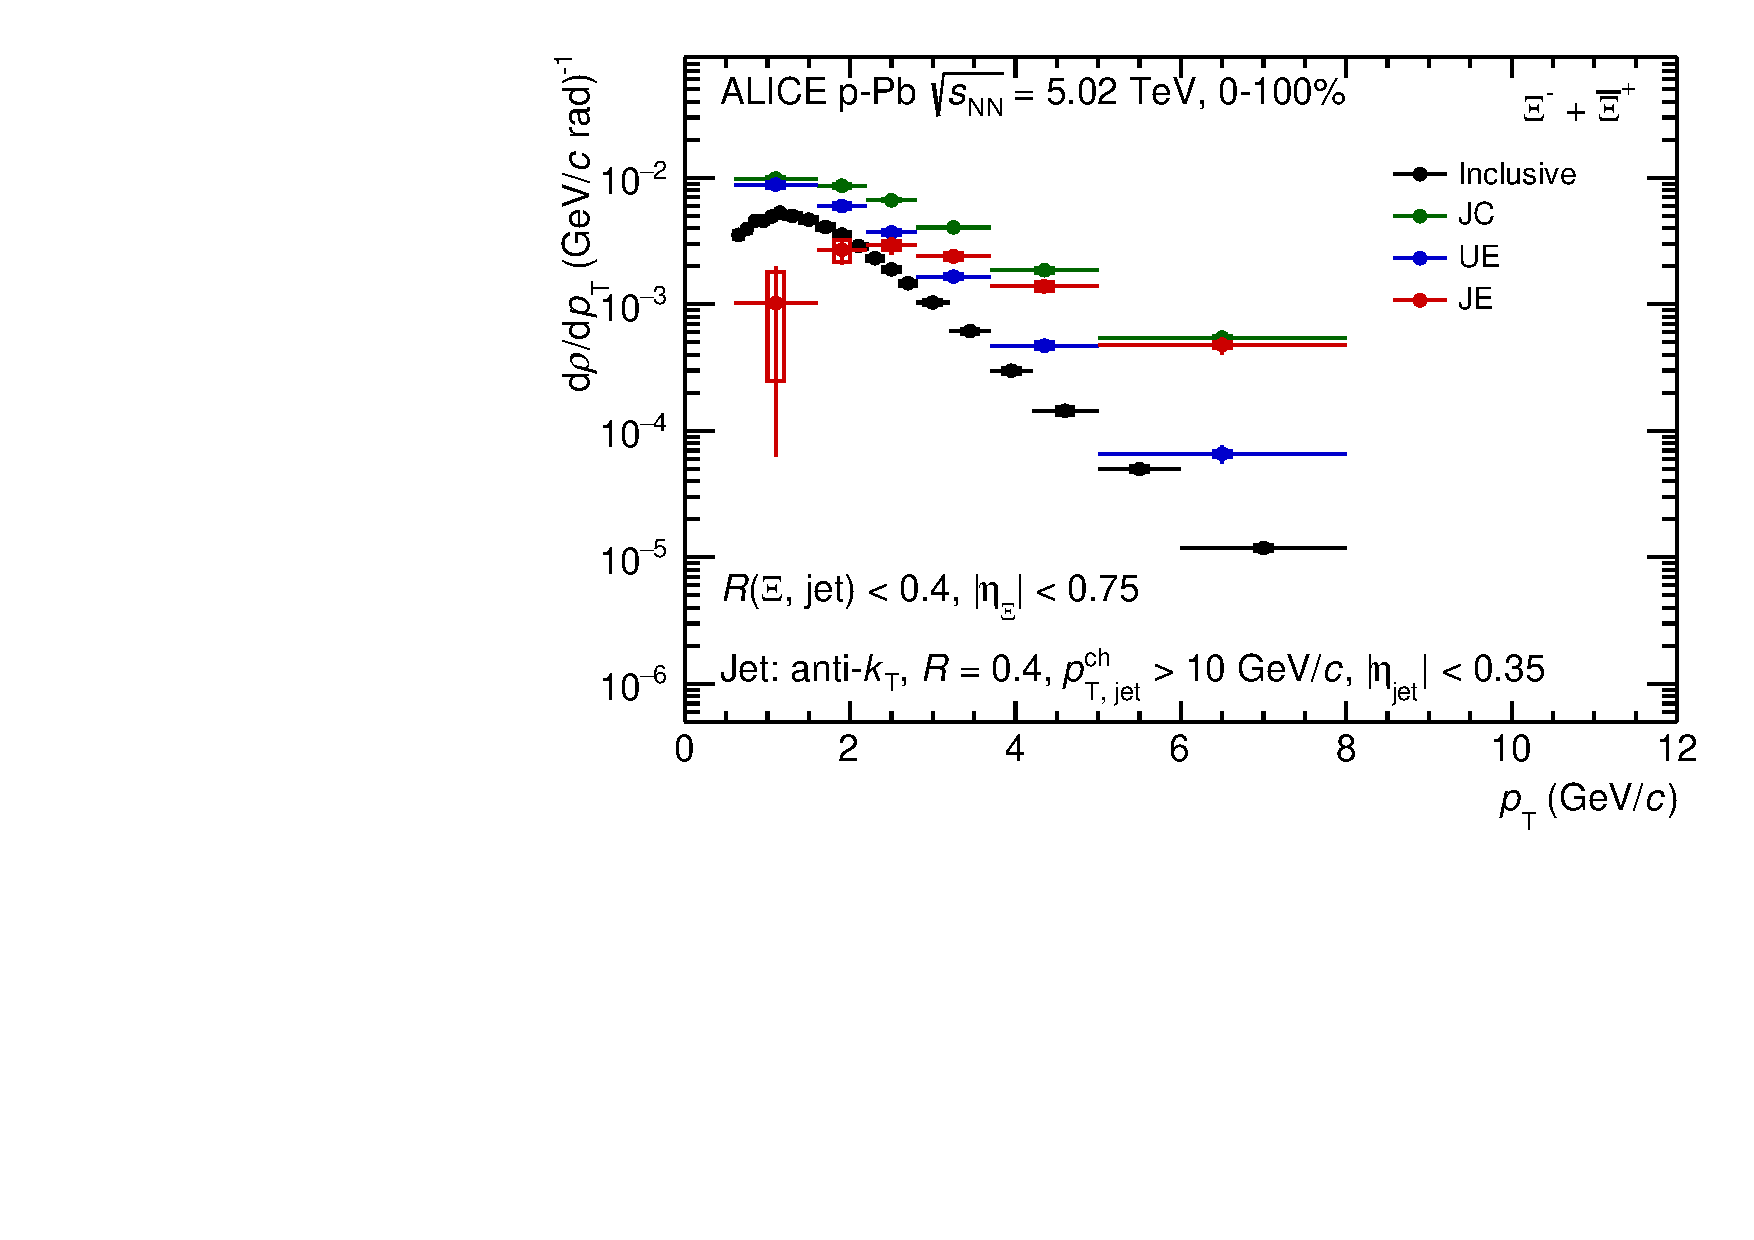
\includegraphics[width=.4\textwidth]{cf5_3}
		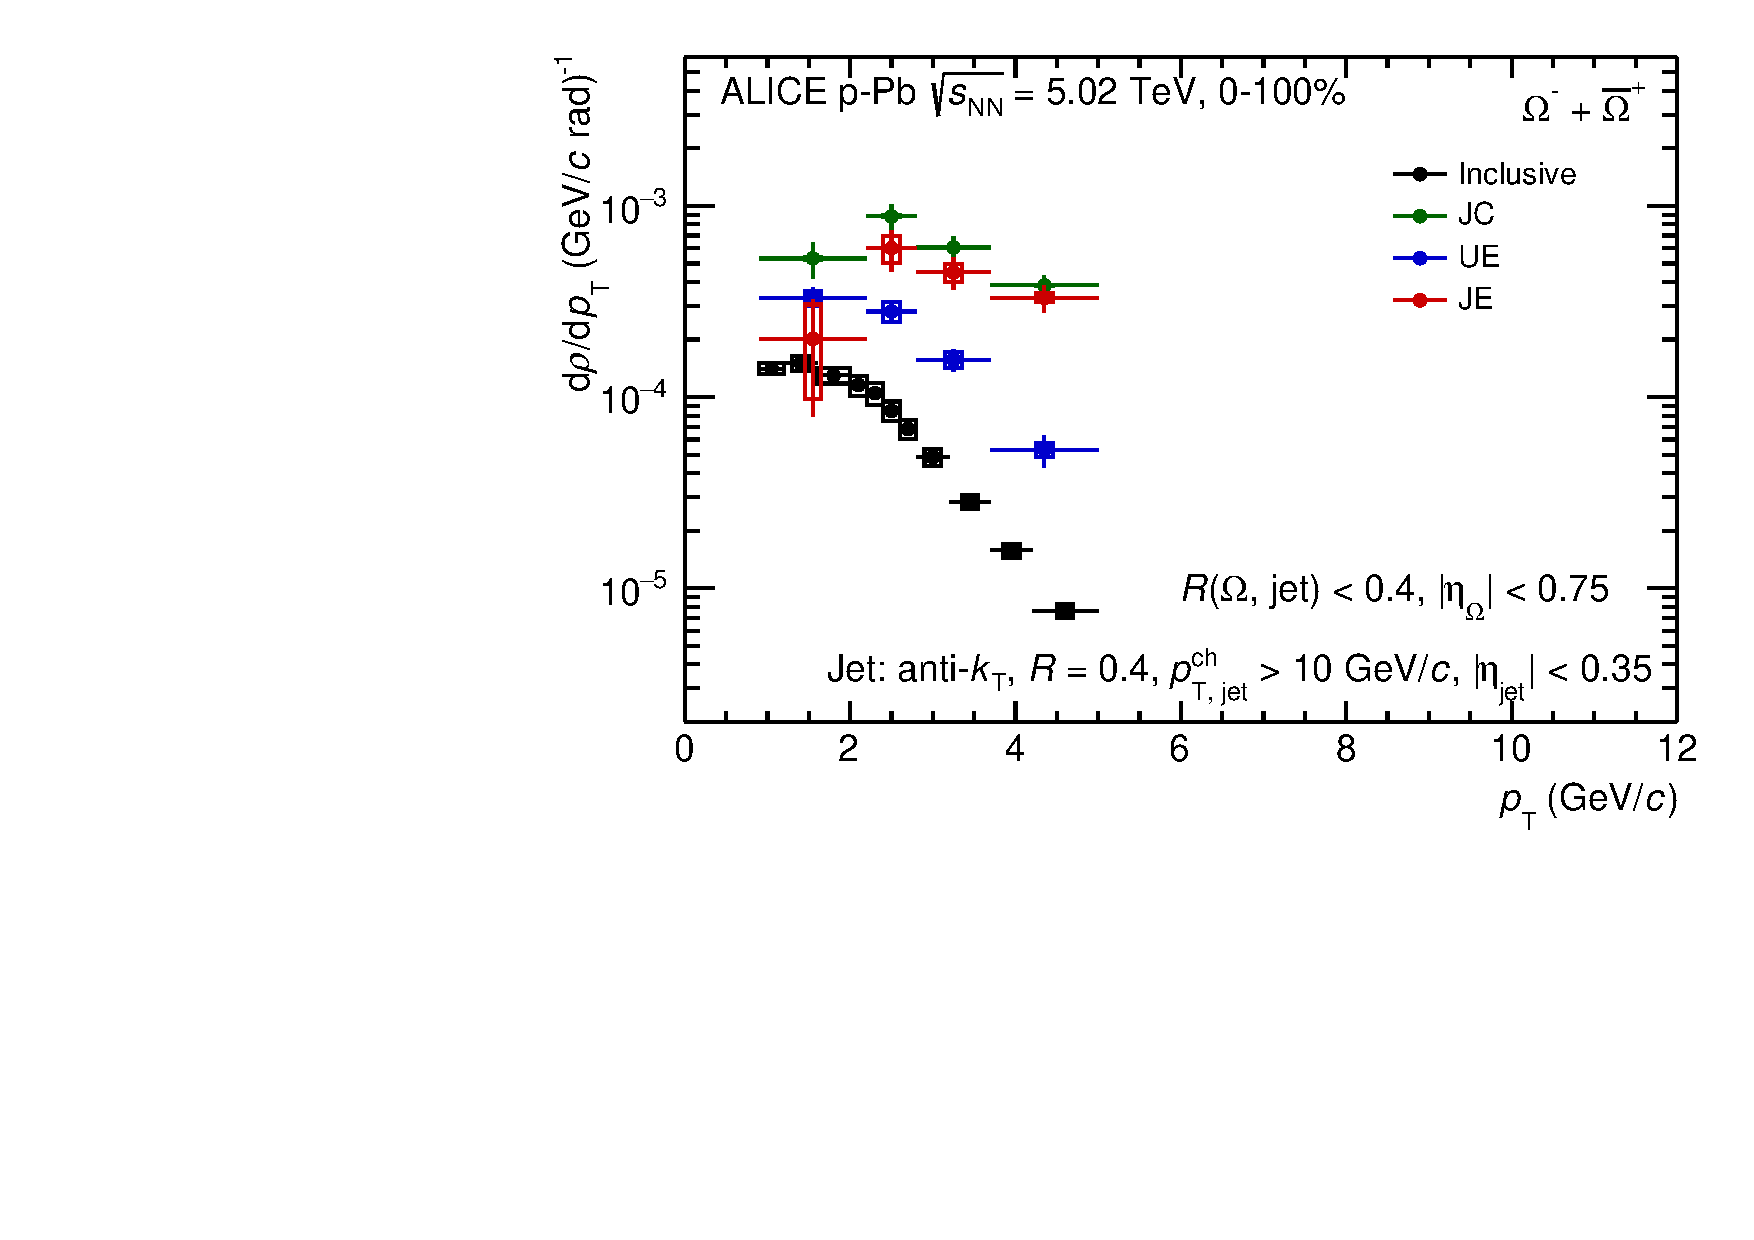
\includegraphics[width=.4\textwidth]{cf5_4}
	\end{center}
	\caption{$\pT$-differential density of $\kzero$, $\lmb + \almb$, $\X + \Ix$ and $\Om + \Mo$ in 0-100\% in \pPb at \fivenn. In those plots, the black point depicts particles witch from minimum bias events, the green point depicts particles which from the jet cones, the blue point depicts particles within perpendicular cone of jet which associated with the underlying event and the red point depicts the particle from the jet fragmentation.}
	\label{fig:pPbSpect}
\end{figure}

The $\pT$ distributions of $\kzero$, $\lmb + \almb$ and $\X + \Ix$ for the event classes defined in Tab.~\ref{tab:multi} are show in Fig.~\ref{fig:pPbSpectwCent}. The inclusive distributions become harder with increasing charged-particle multiplicity. Particles in JE, which generated by jet fragmentation, are systematically independent with centrality classes.
\begin{figure}[!ht]
\begin{center}
	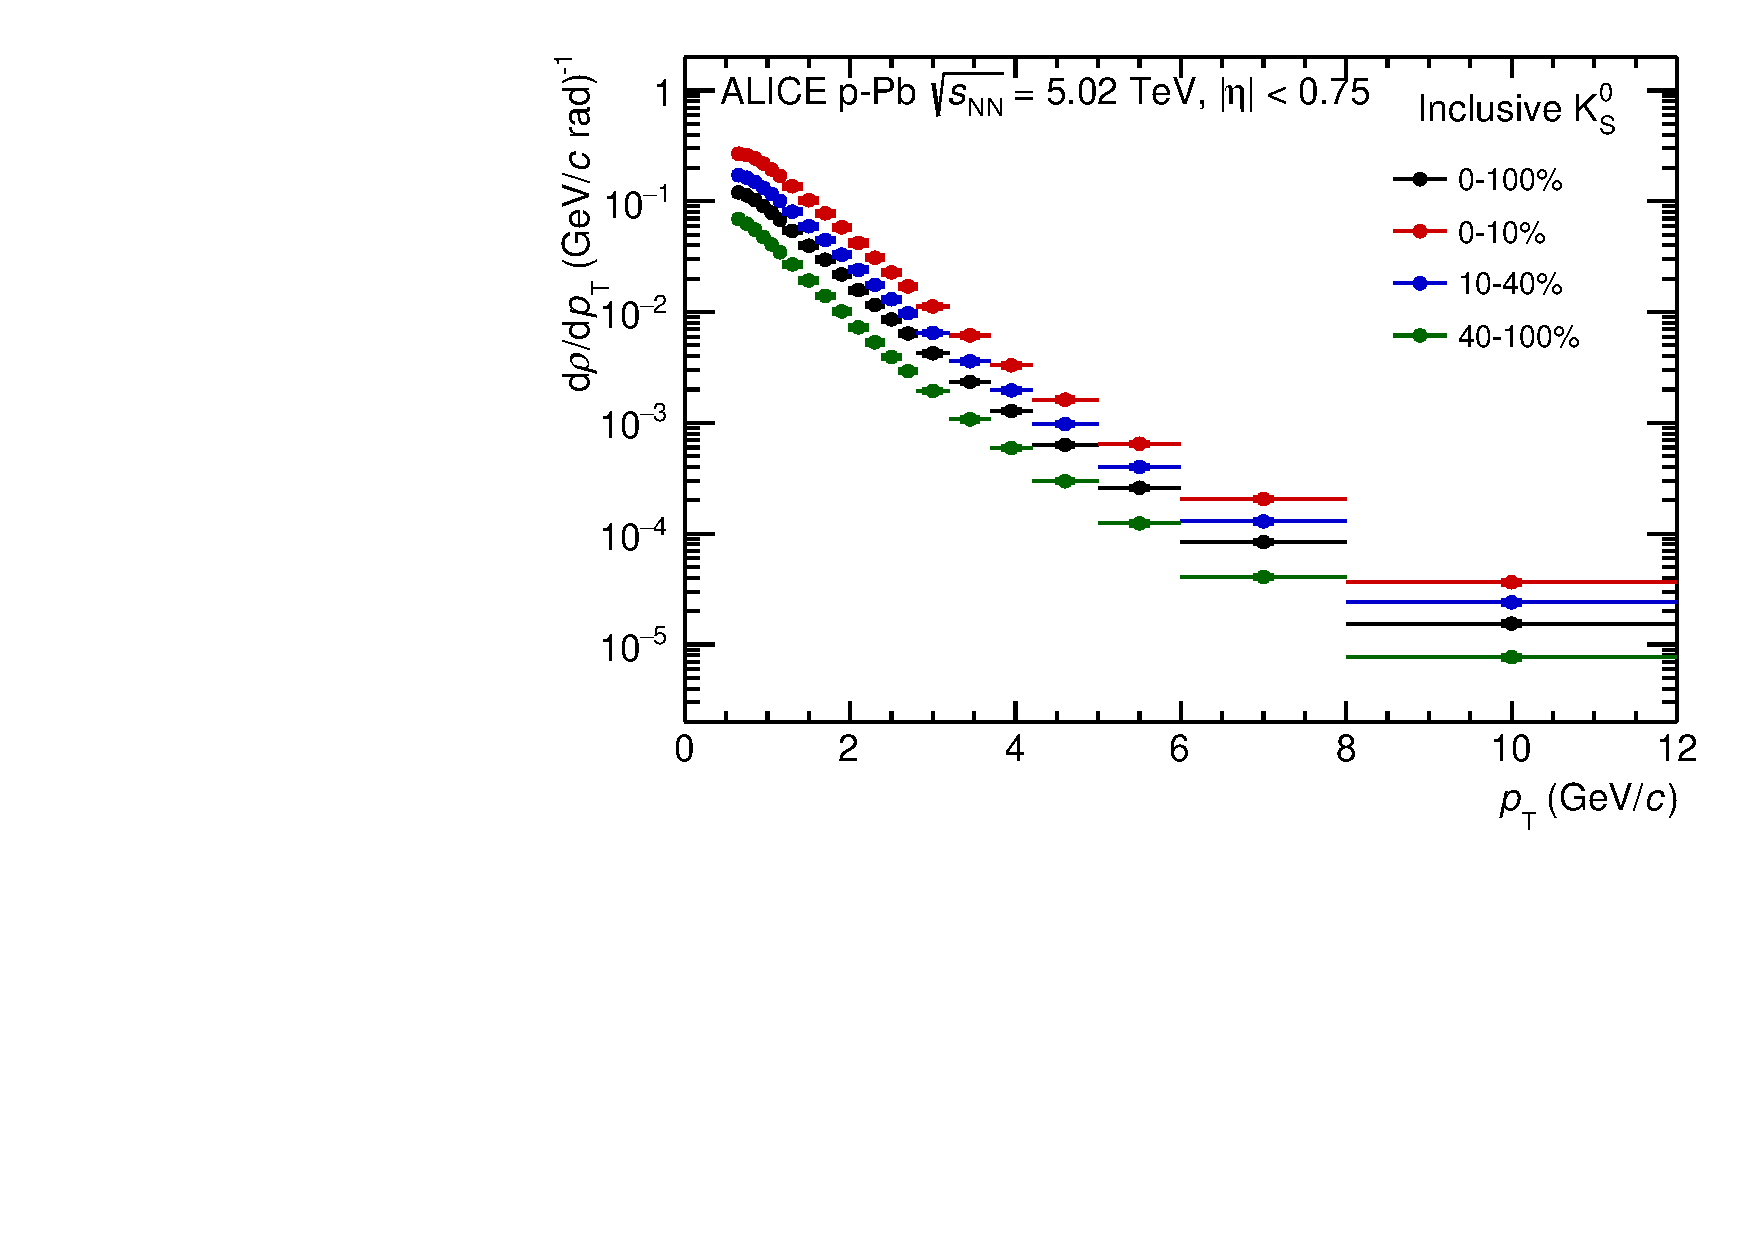
\includegraphics[width=.3\textwidth]{cf6_1}
	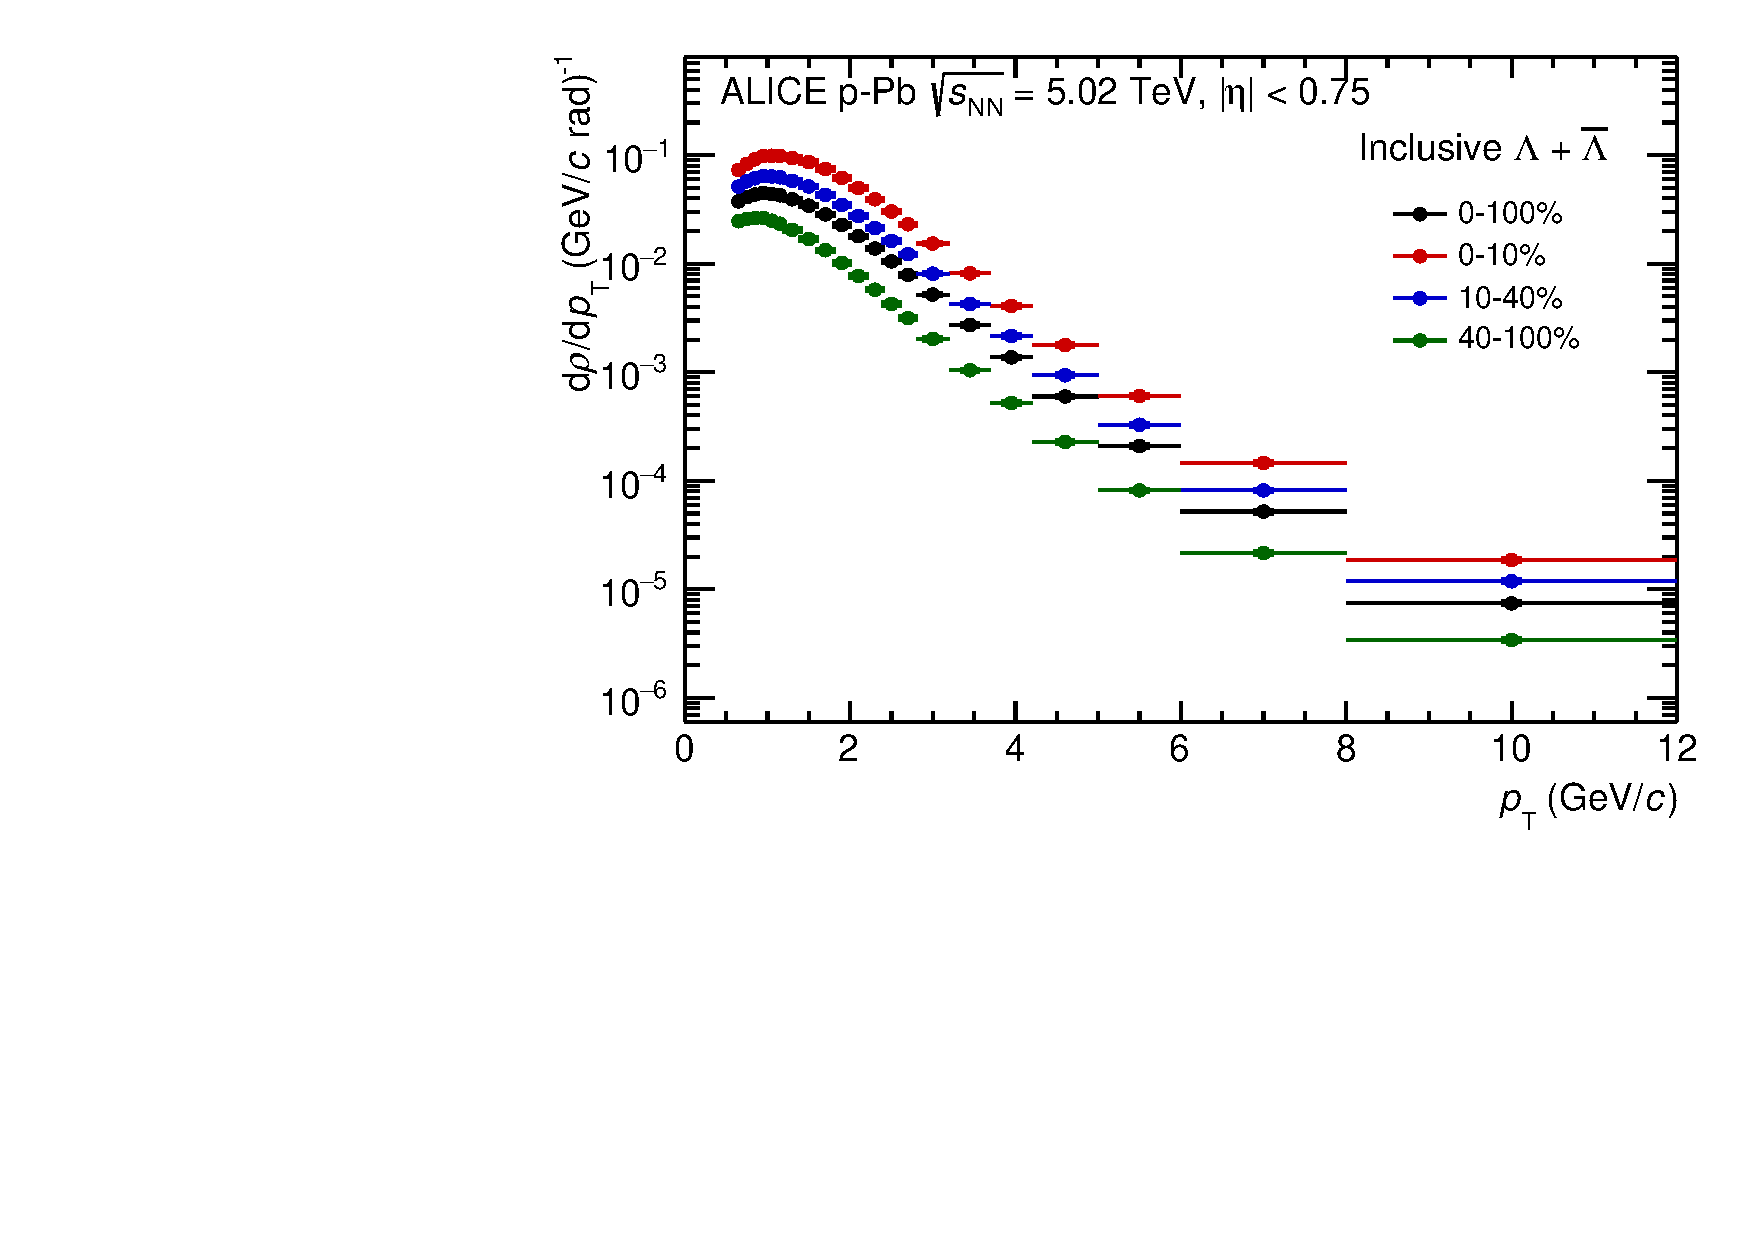
\includegraphics[width=.3\textwidth]{cf6_2}
	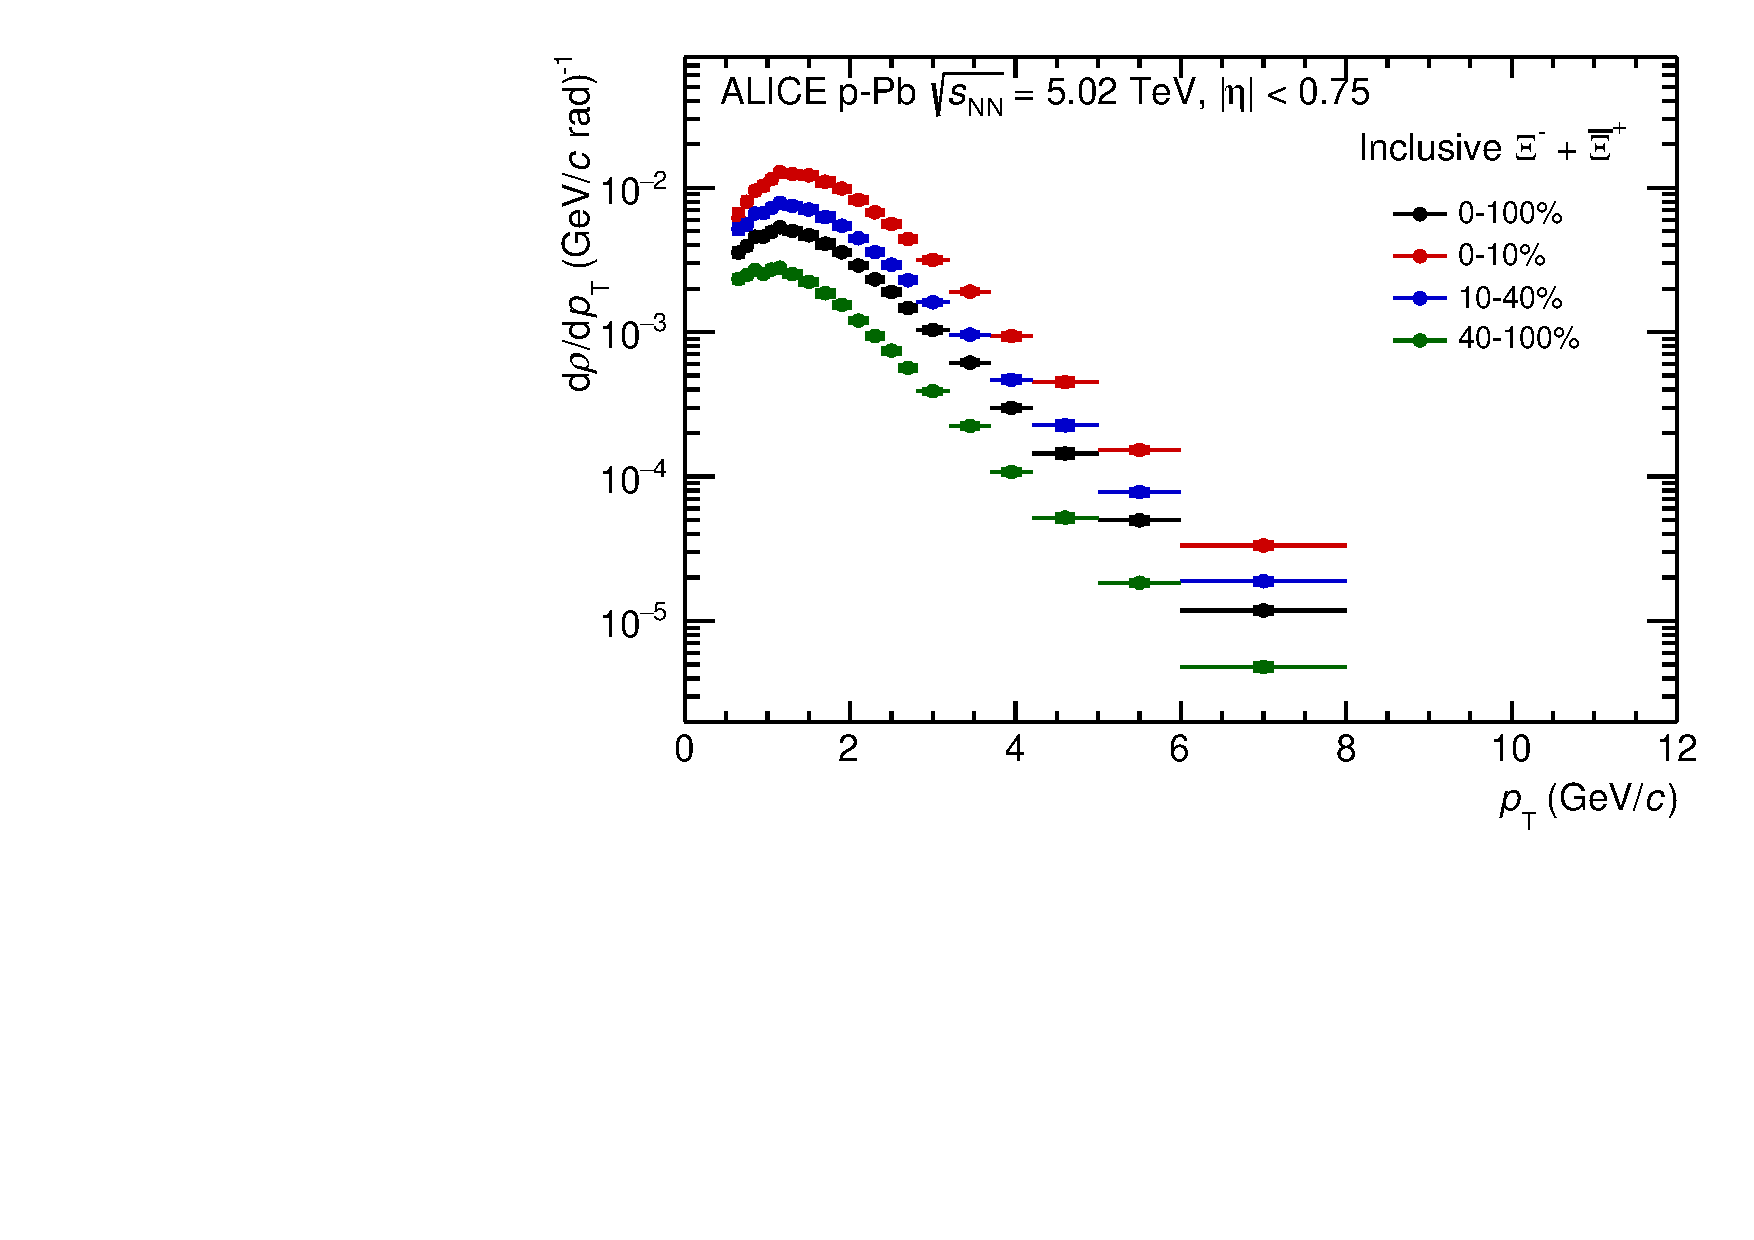
\includegraphics[width=.3\textwidth]{cf6_3}
	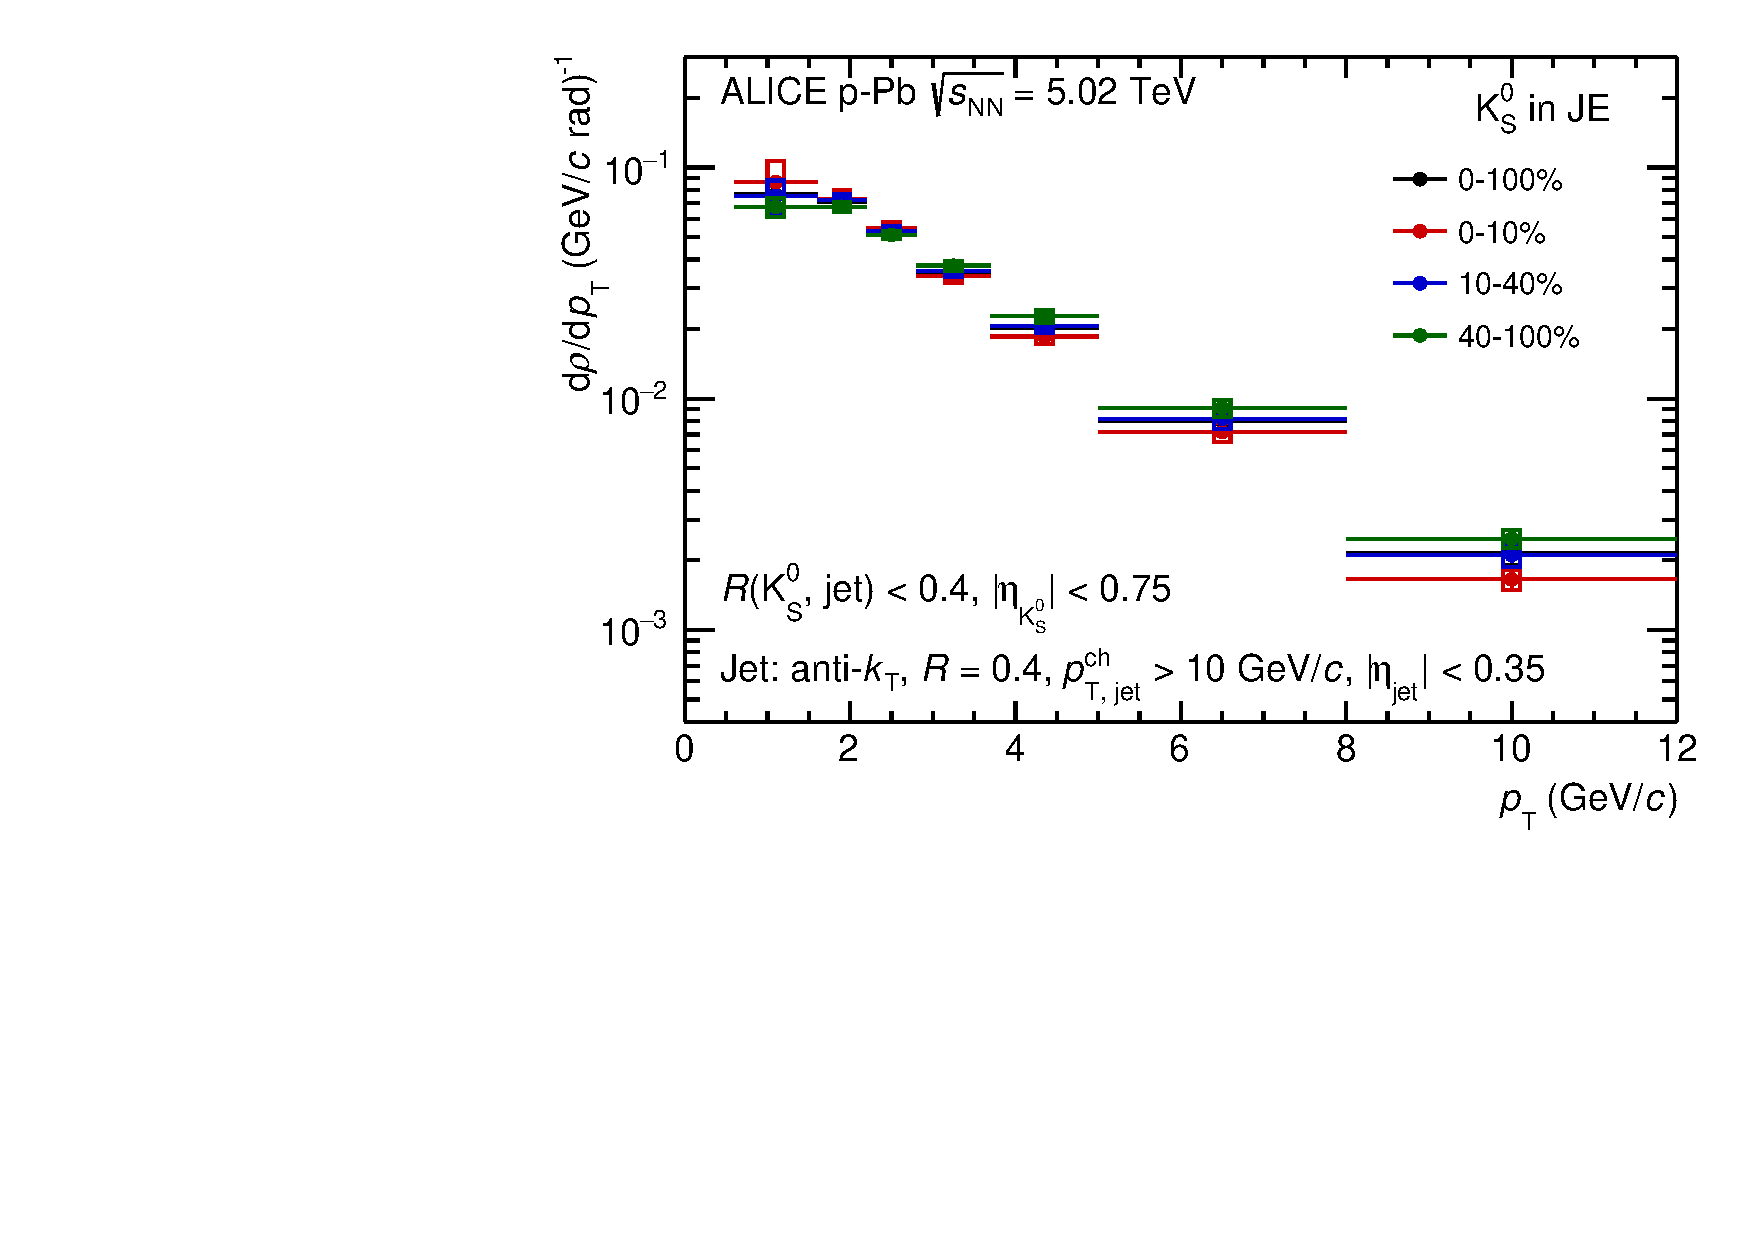
\includegraphics[width=.3\textwidth]{cf6_4}
	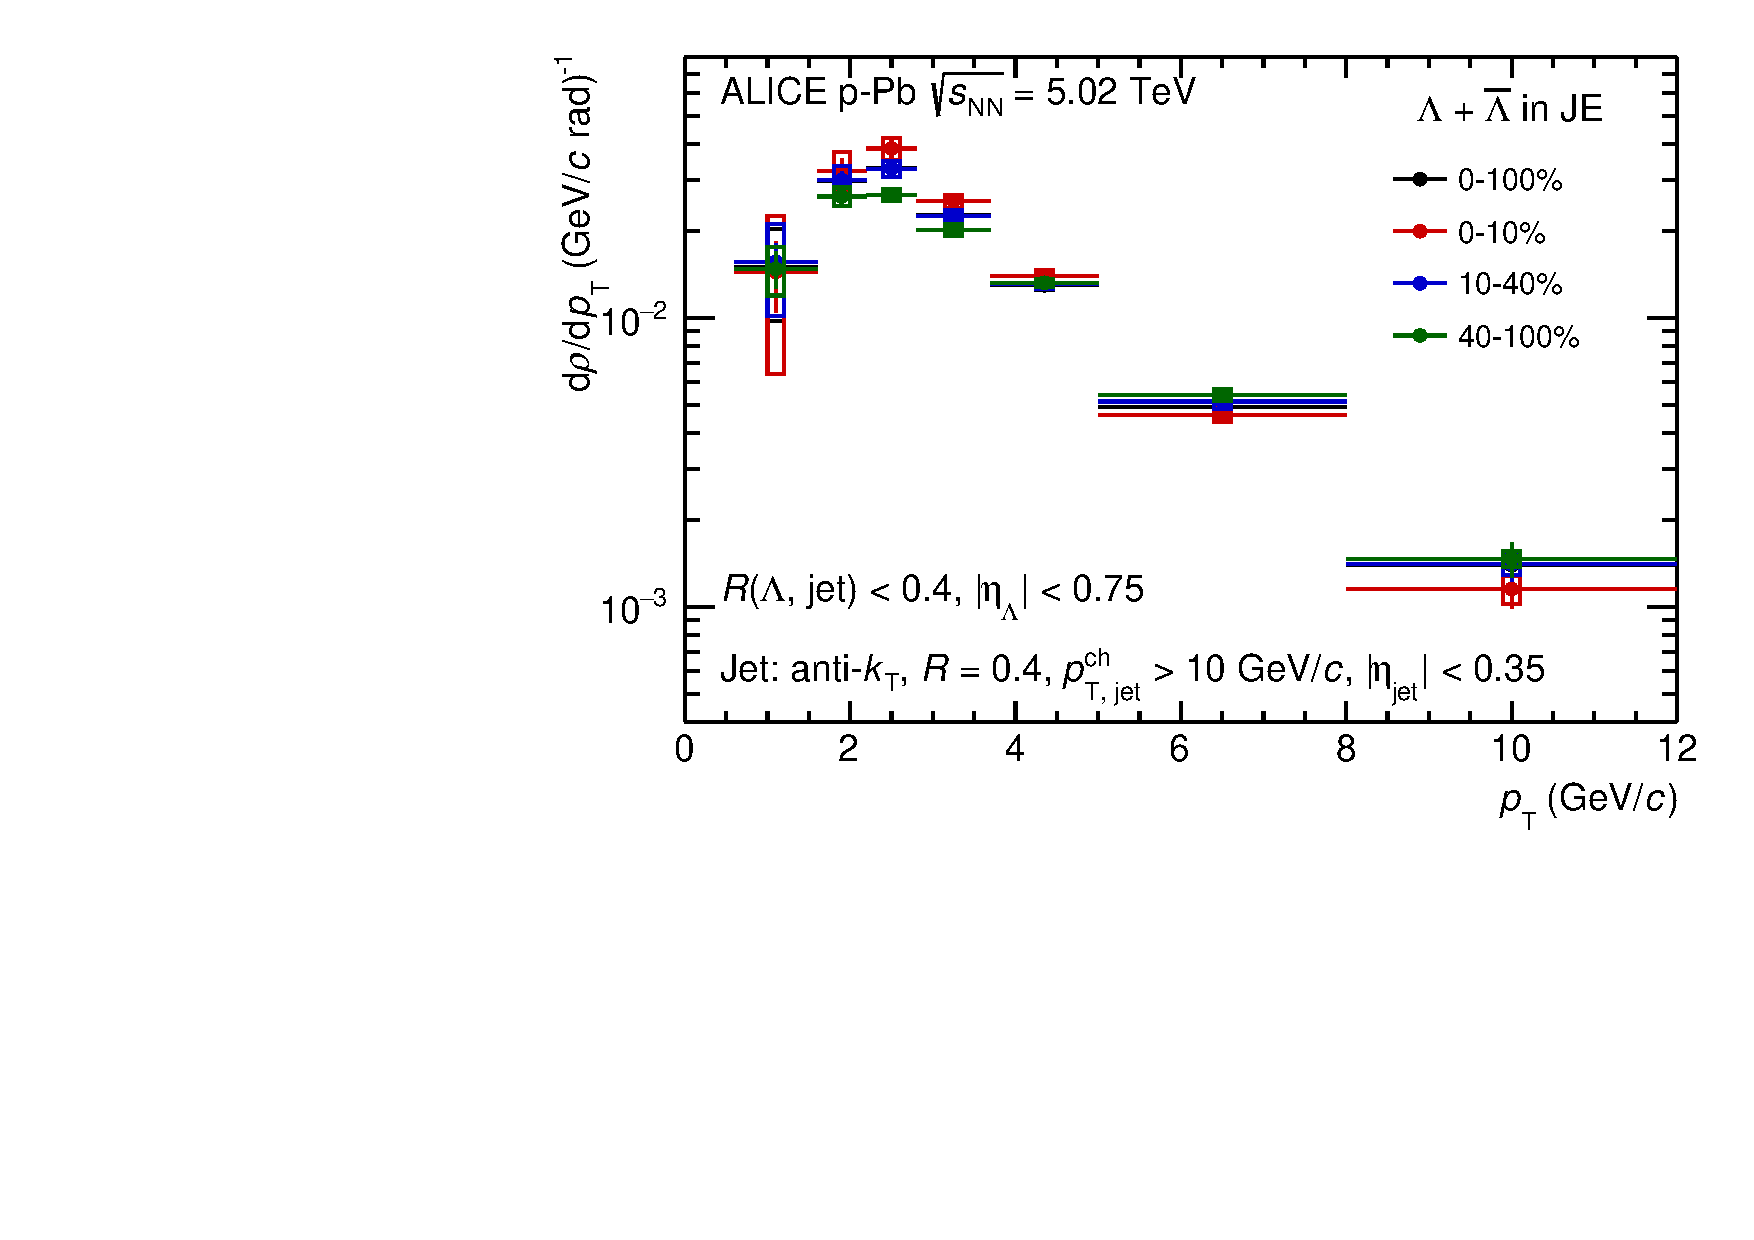
\includegraphics[width=.3\textwidth]{cf6_5}
	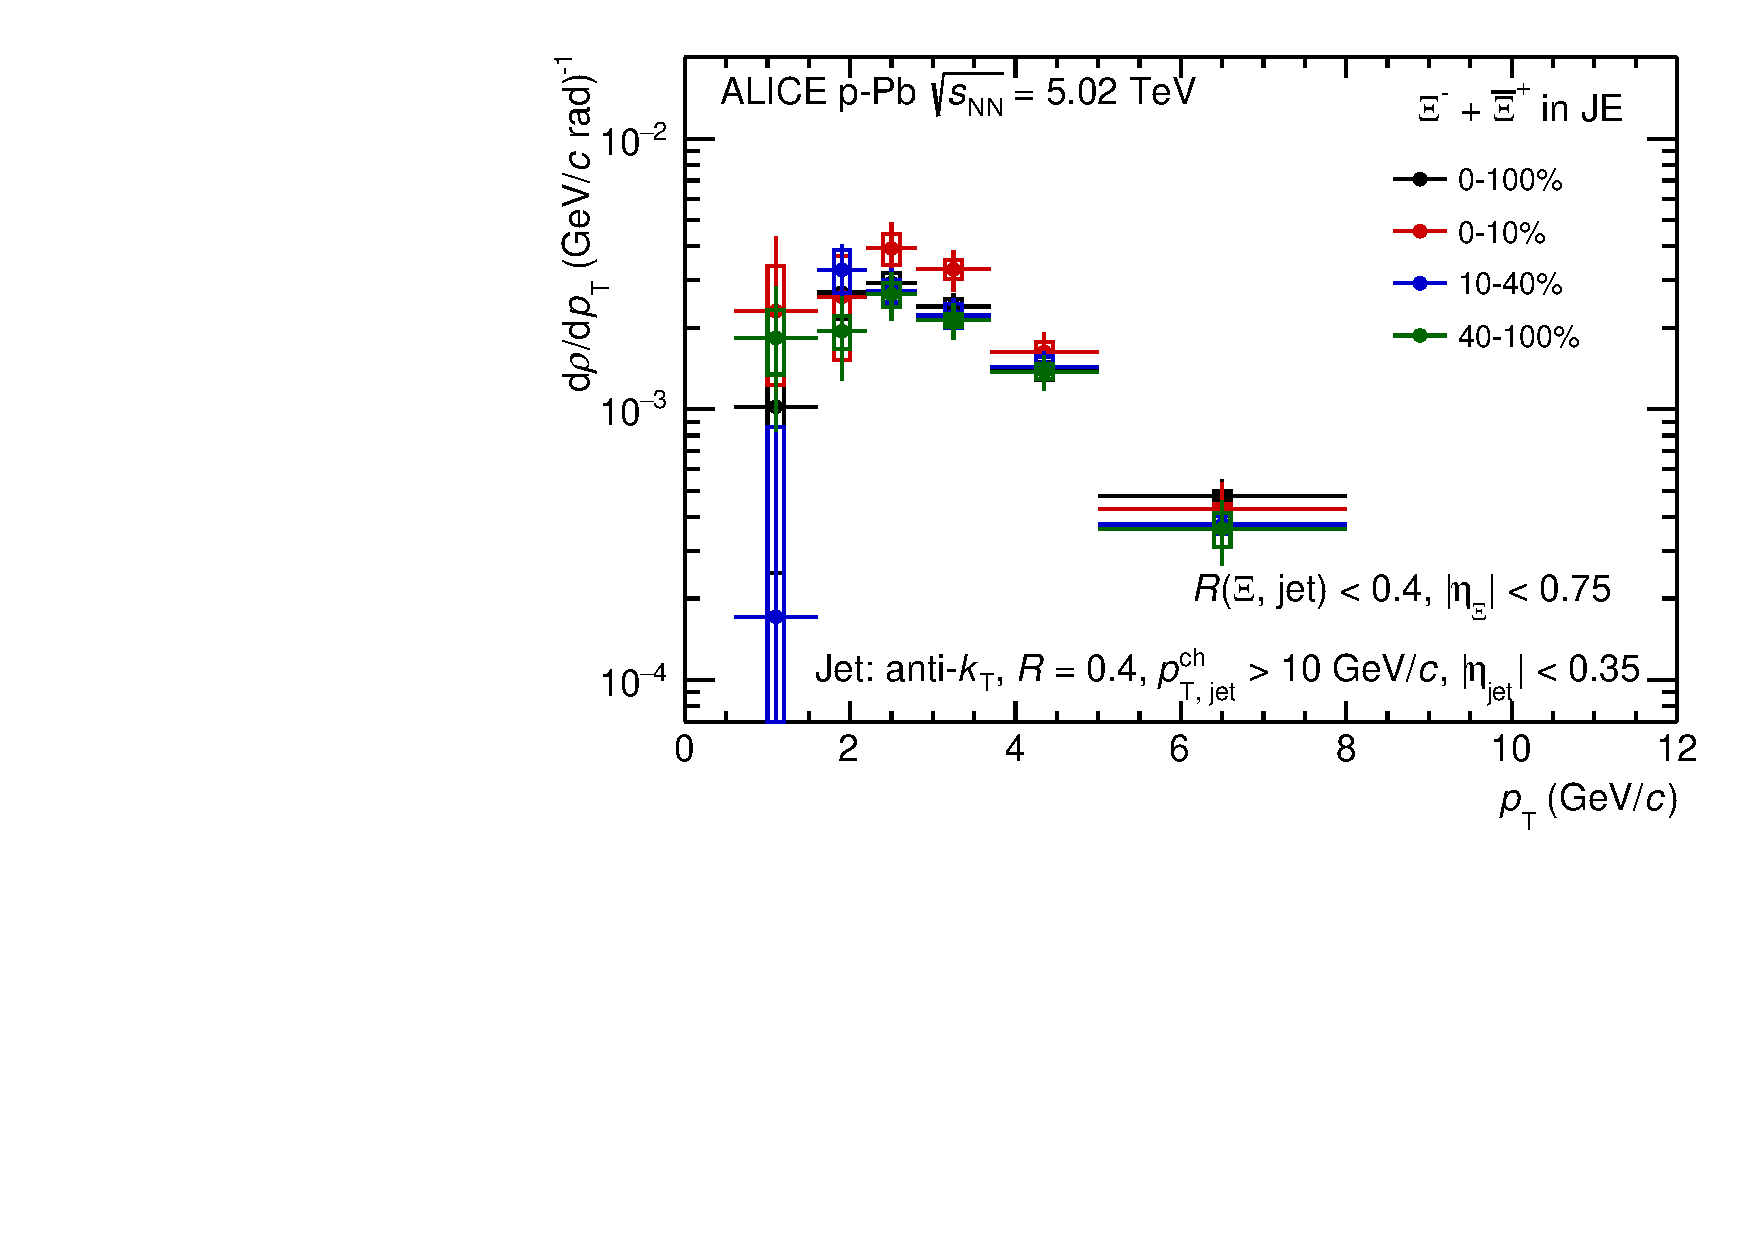
\includegraphics[width=.3\textwidth]{cf6_6}
\end{center}
\caption{$\pT$-differential density of $\kzero$, $\lmb + \almb$ and $\X + \Ix$ in different V0A event centrality classes in \pPb at \fivenn. Top panels show the inclusive particle and bottom panels show particles generated by jet fragmentation. The different centrality classes are depicted with different color.}
\label{fig:pPbSpectwCent}
\end{figure}

\subsection{Baryon-to-meson and baryon-to-baryon ratios}
\label{subsec:ParRatios}
The baryon-to-meson and baryon-to-baryon ratios in \pp and MB \pPb collisions are displayed in Fig.~\ref{fig:ppRatio} and \ref{fig:pPbRatio}.

\begin{figure}[!ht]
	\begin{center}
		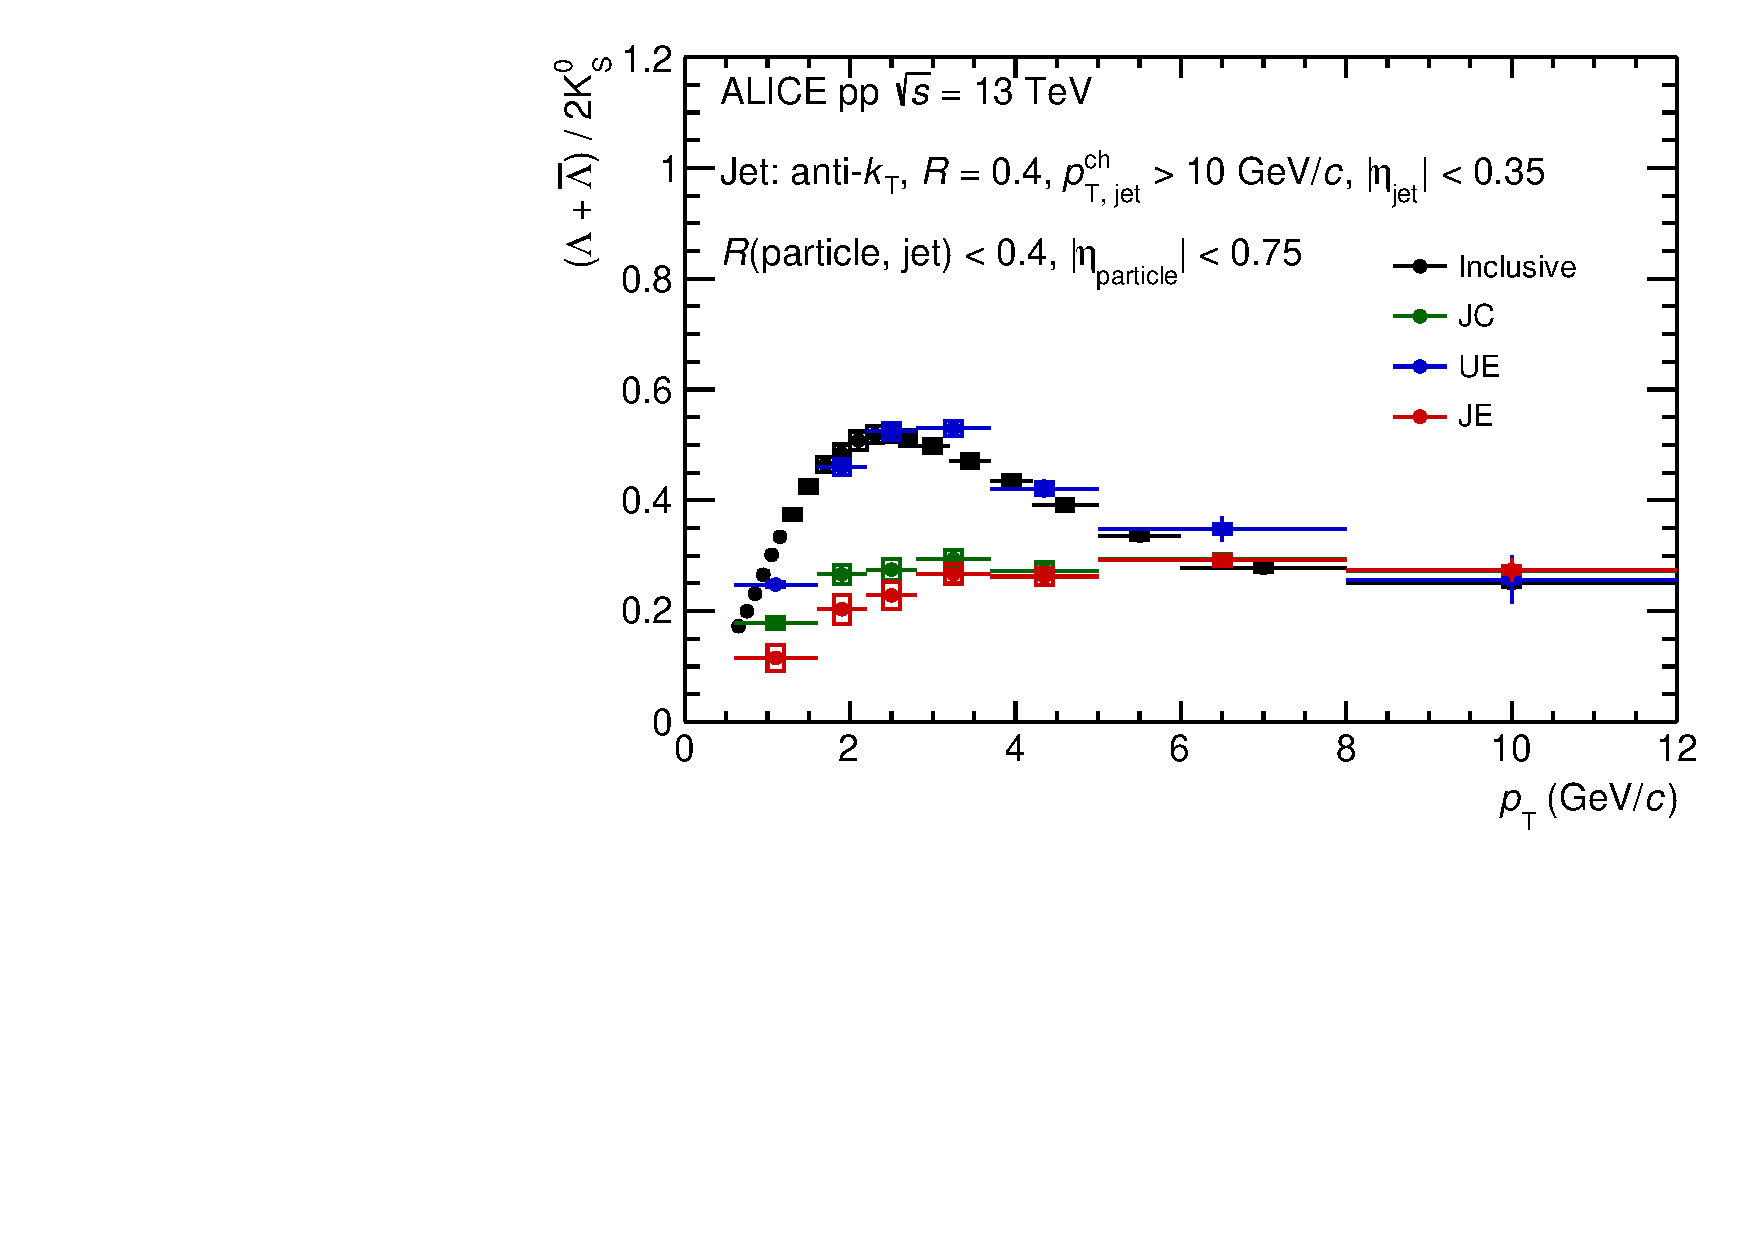
\includegraphics[width=.3\textwidth]{cf7_1}
		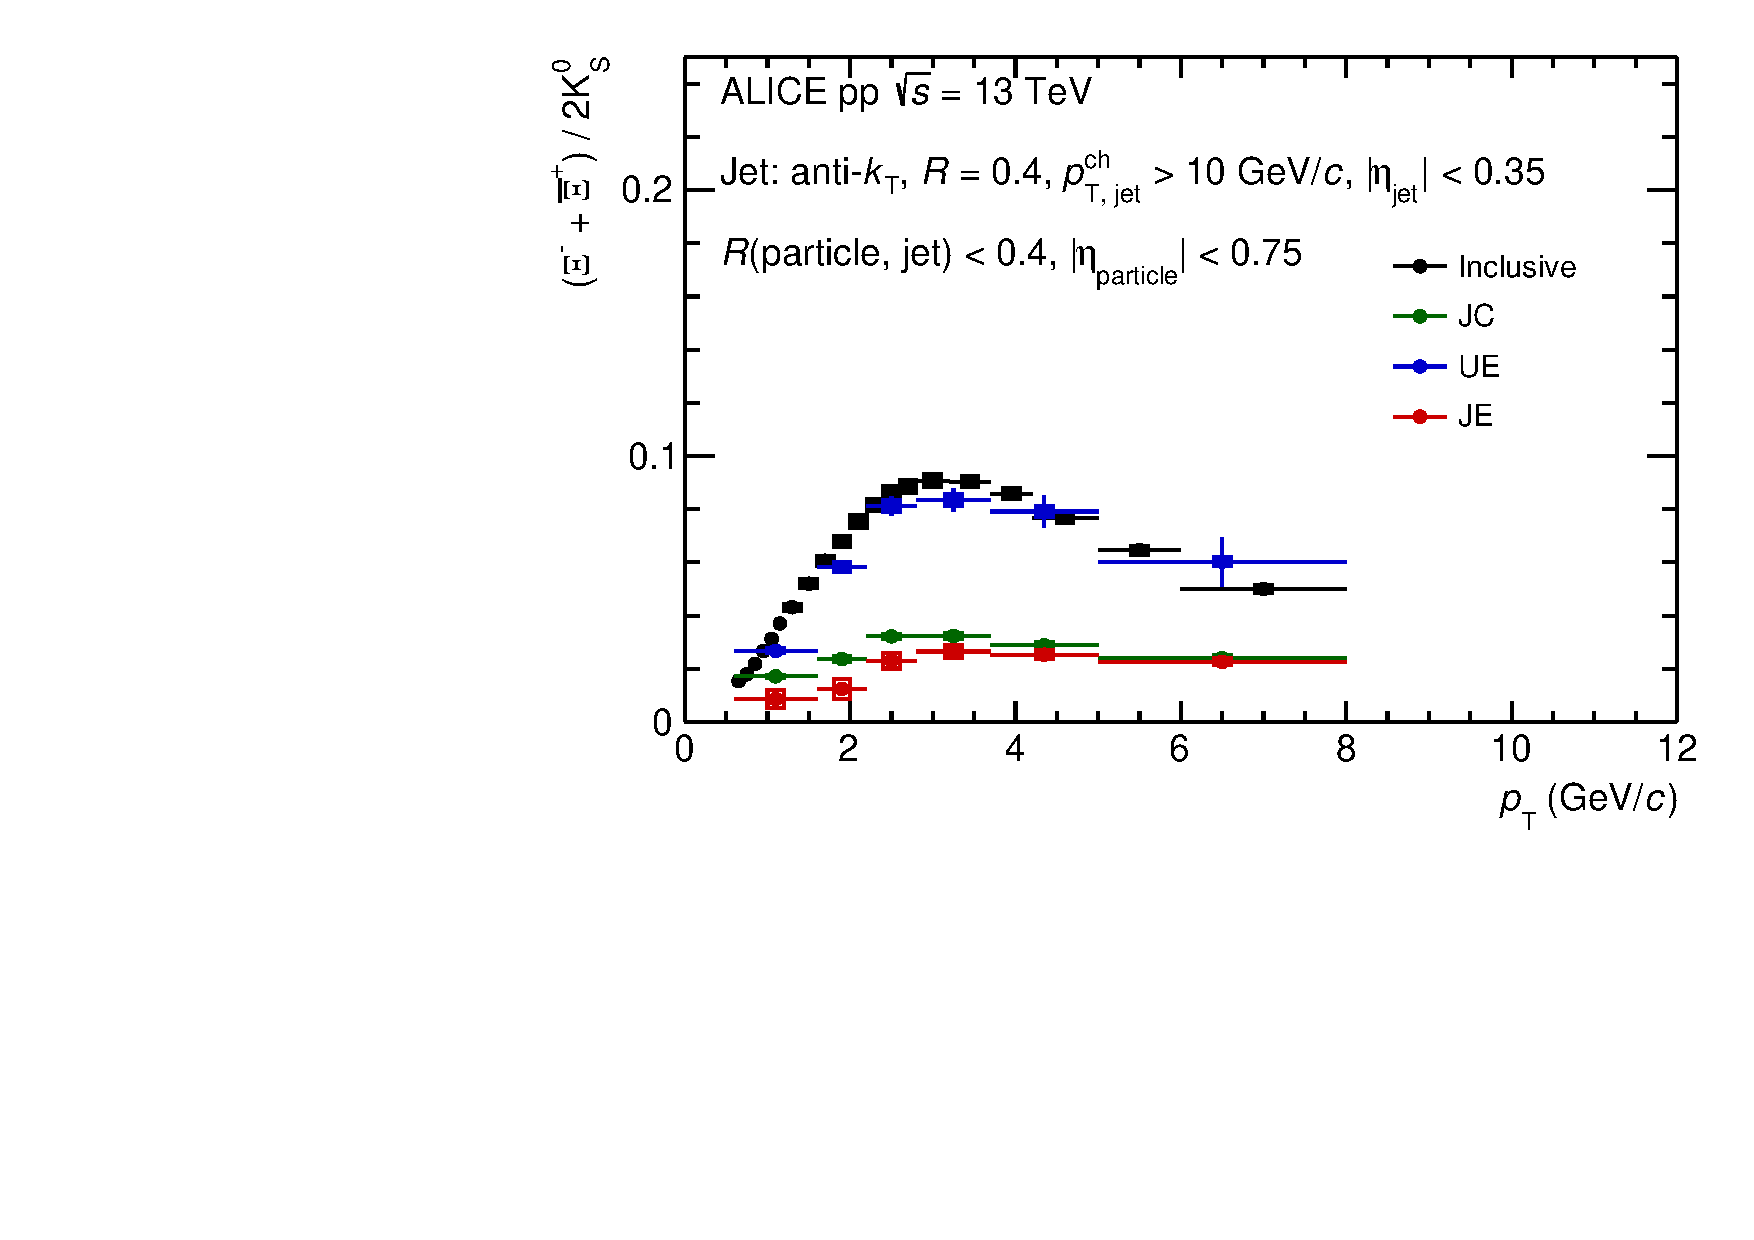
\includegraphics[width=.3\textwidth]{cf7_2}
		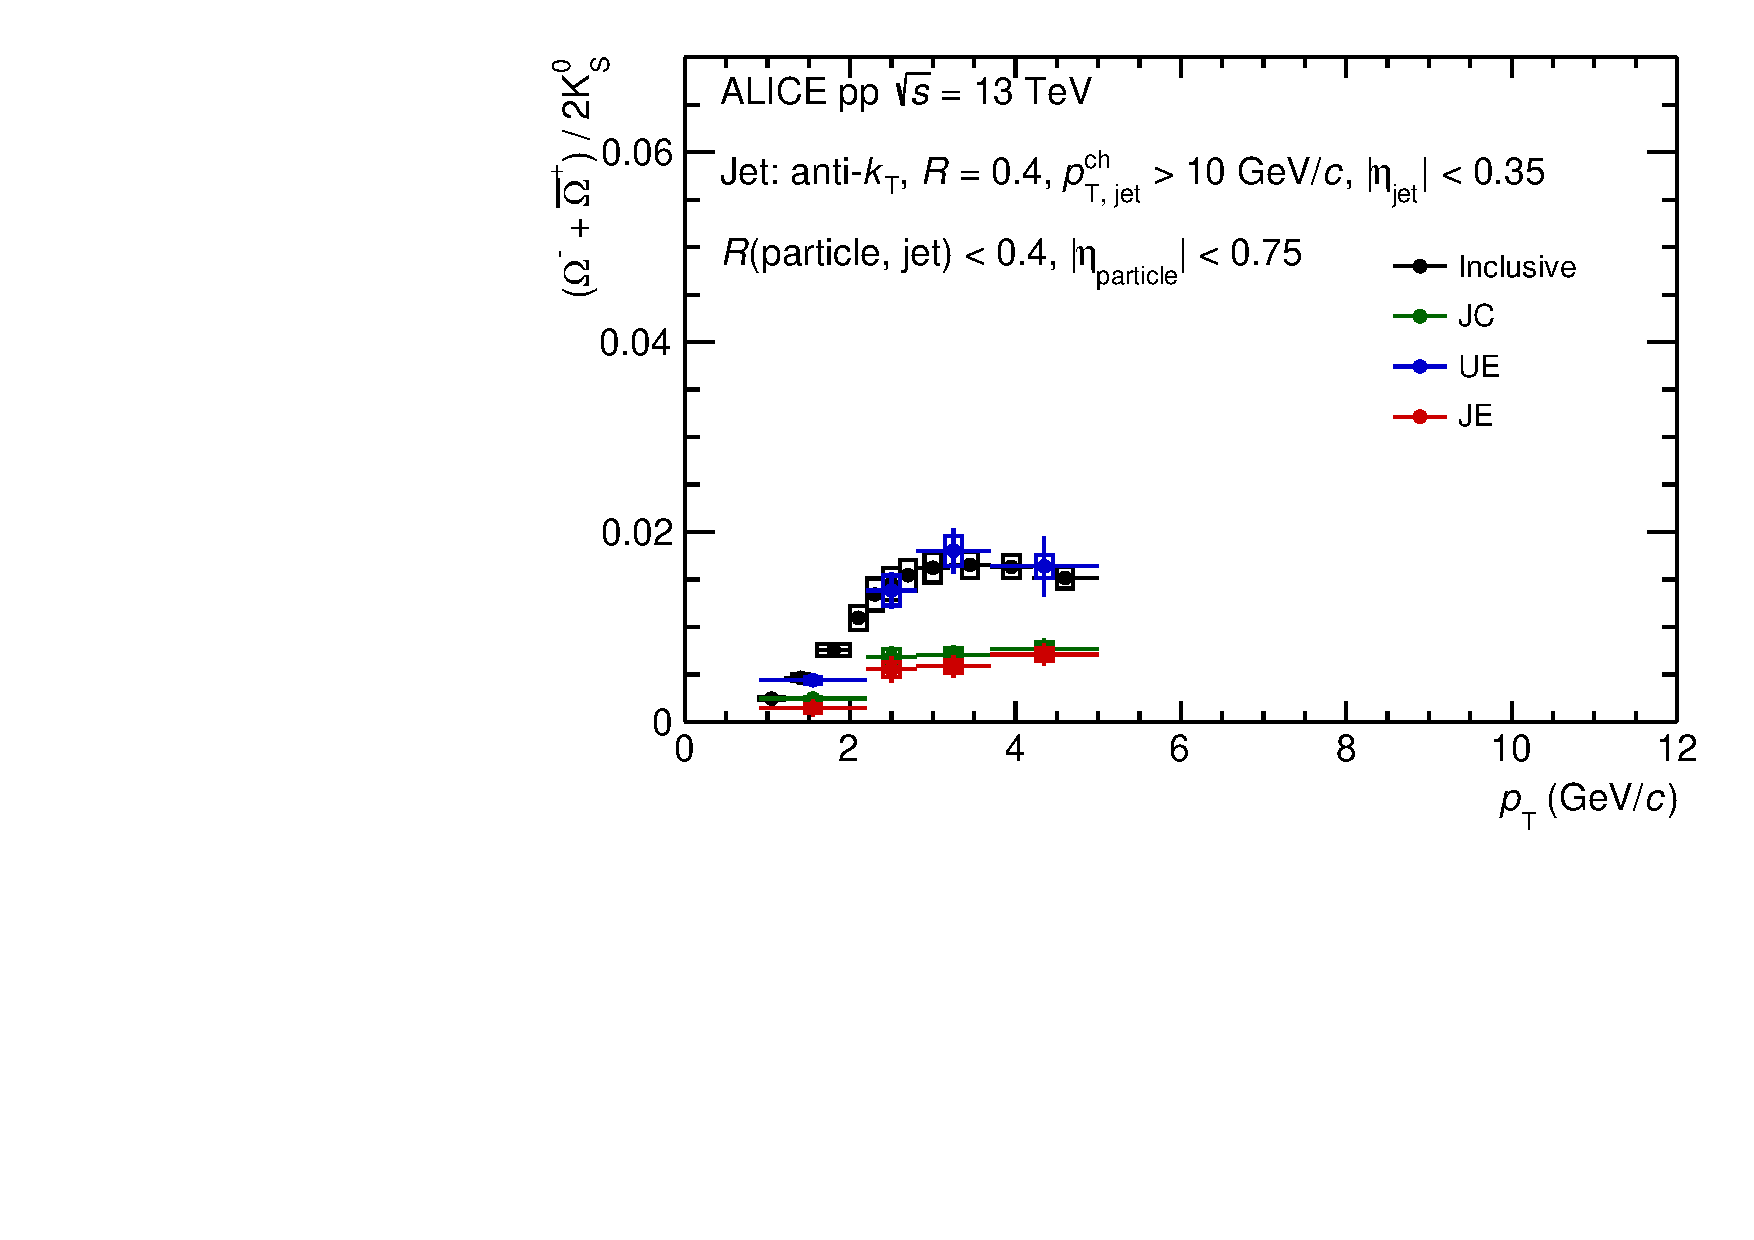
\includegraphics[width=.3\textwidth]{cf7_3}
		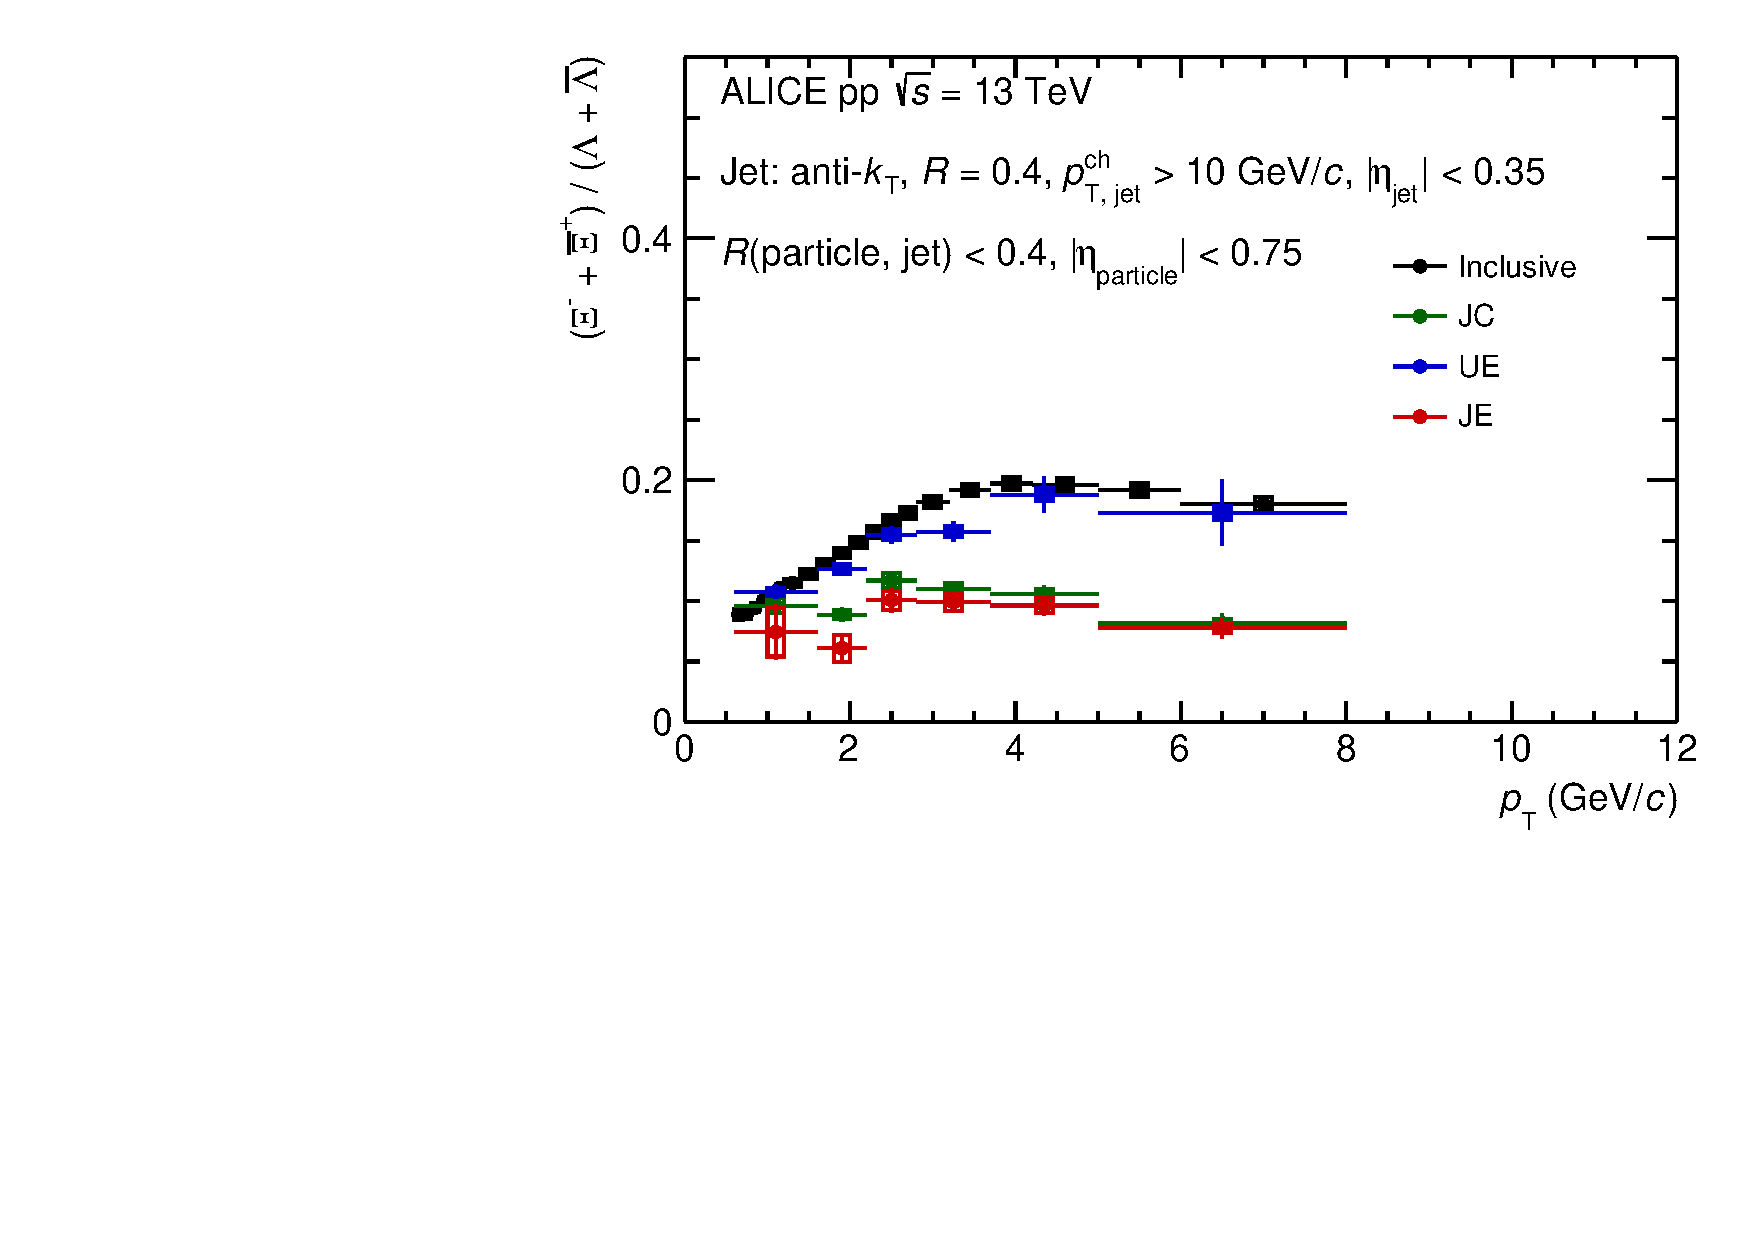
\includegraphics[width=.3\textwidth]{cf7_4}
		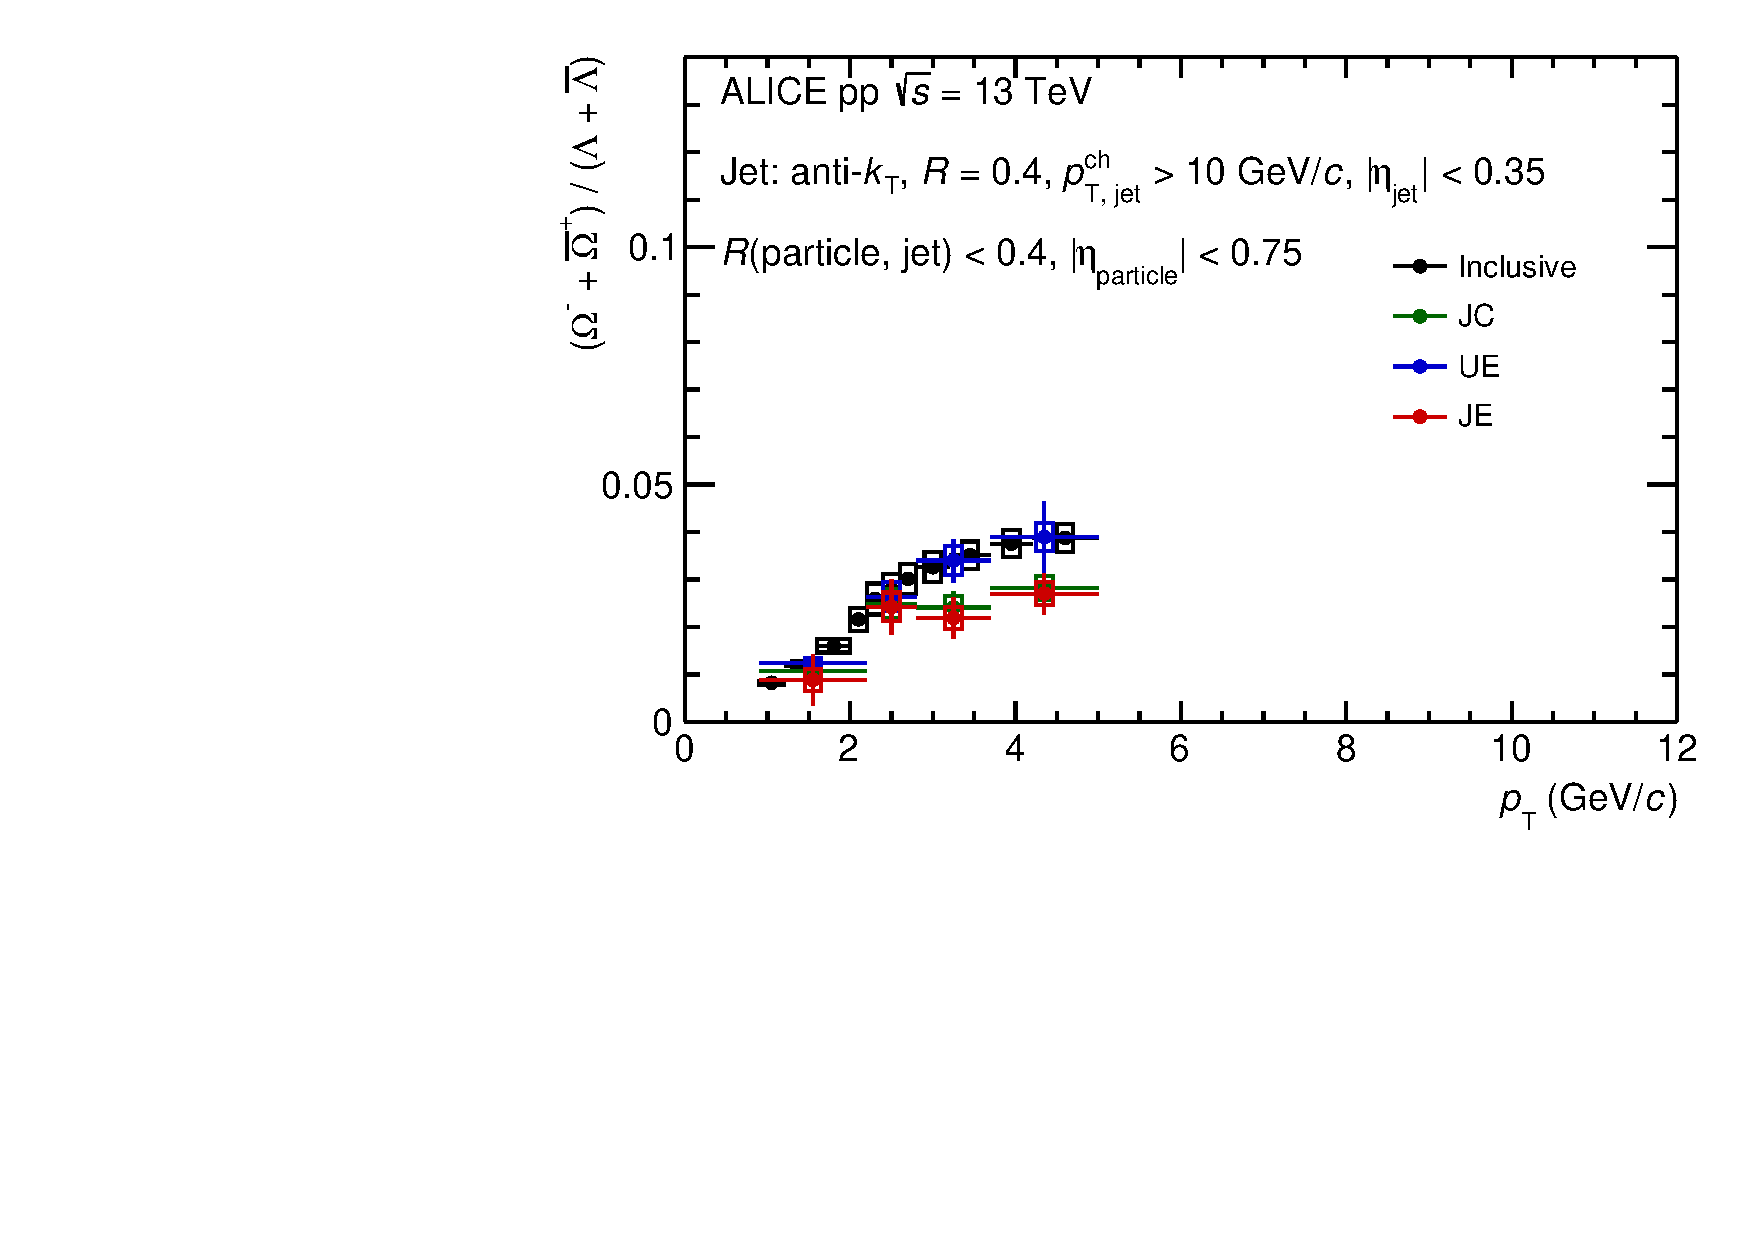
\includegraphics[width=.3\textwidth]{cf7_5}
		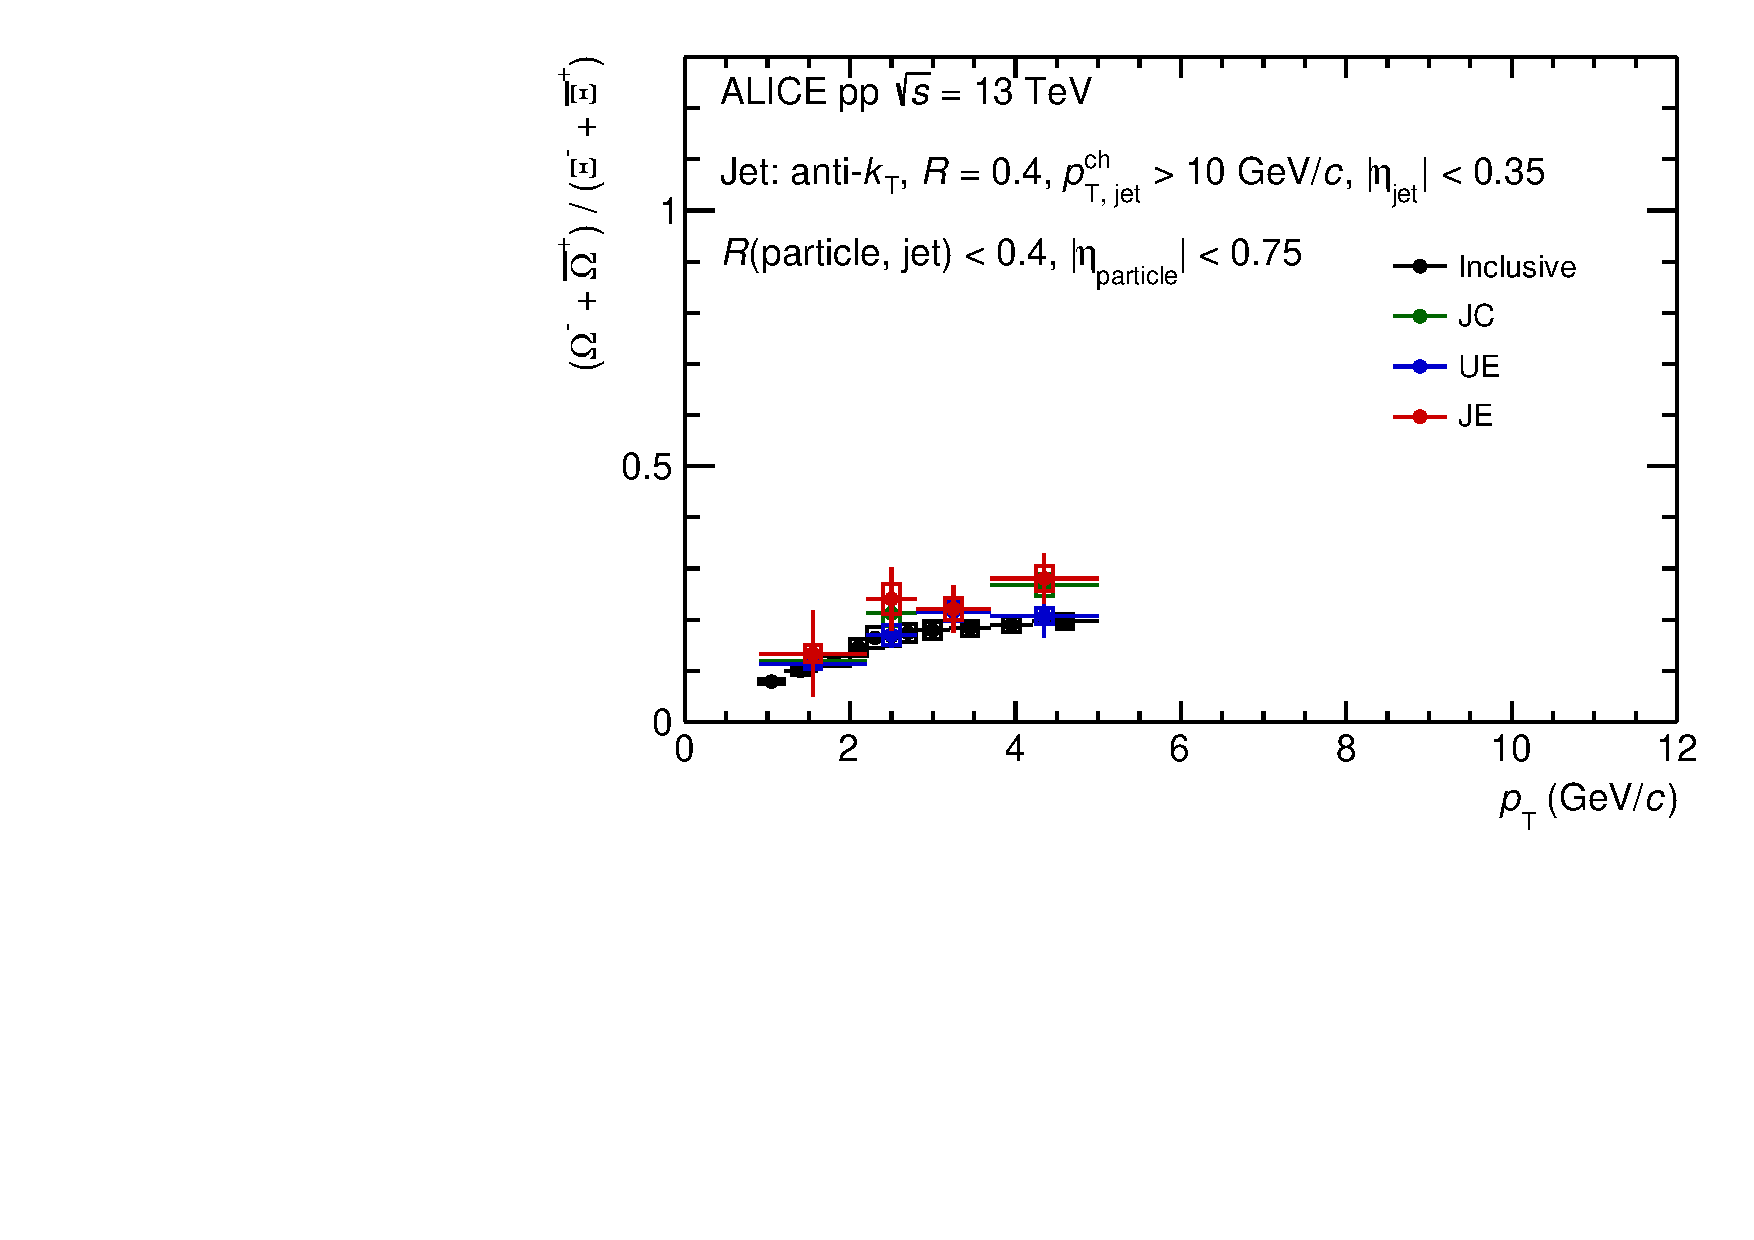
\includegraphics[width=.3\textwidth]{cf7_6}
	\end{center}
	\caption{The baryon-to-meson ($\lmb/\kzero$, $\Xi/\kzero$ and $\Omega/\kzero$) and baryon-to-baryon($\Xi/\lmb$, $\Omega/\lmb$ and $\Omega/\Xi$) ratio as a function of particle $\pT$ in \pp collisions at \thirteen. In those panels, the black point shows the ratio with particles from minimum bias events, the green point shows the ratio with particles from the jet cones, the blue point shows the ratio with particles from perpendicular cones with jet and the red point shows the ratio with particles that generated by jet.}
	\label{fig:ppRatio}
\end{figure}
\begin{figure}[!ht]
	\begin{center}
		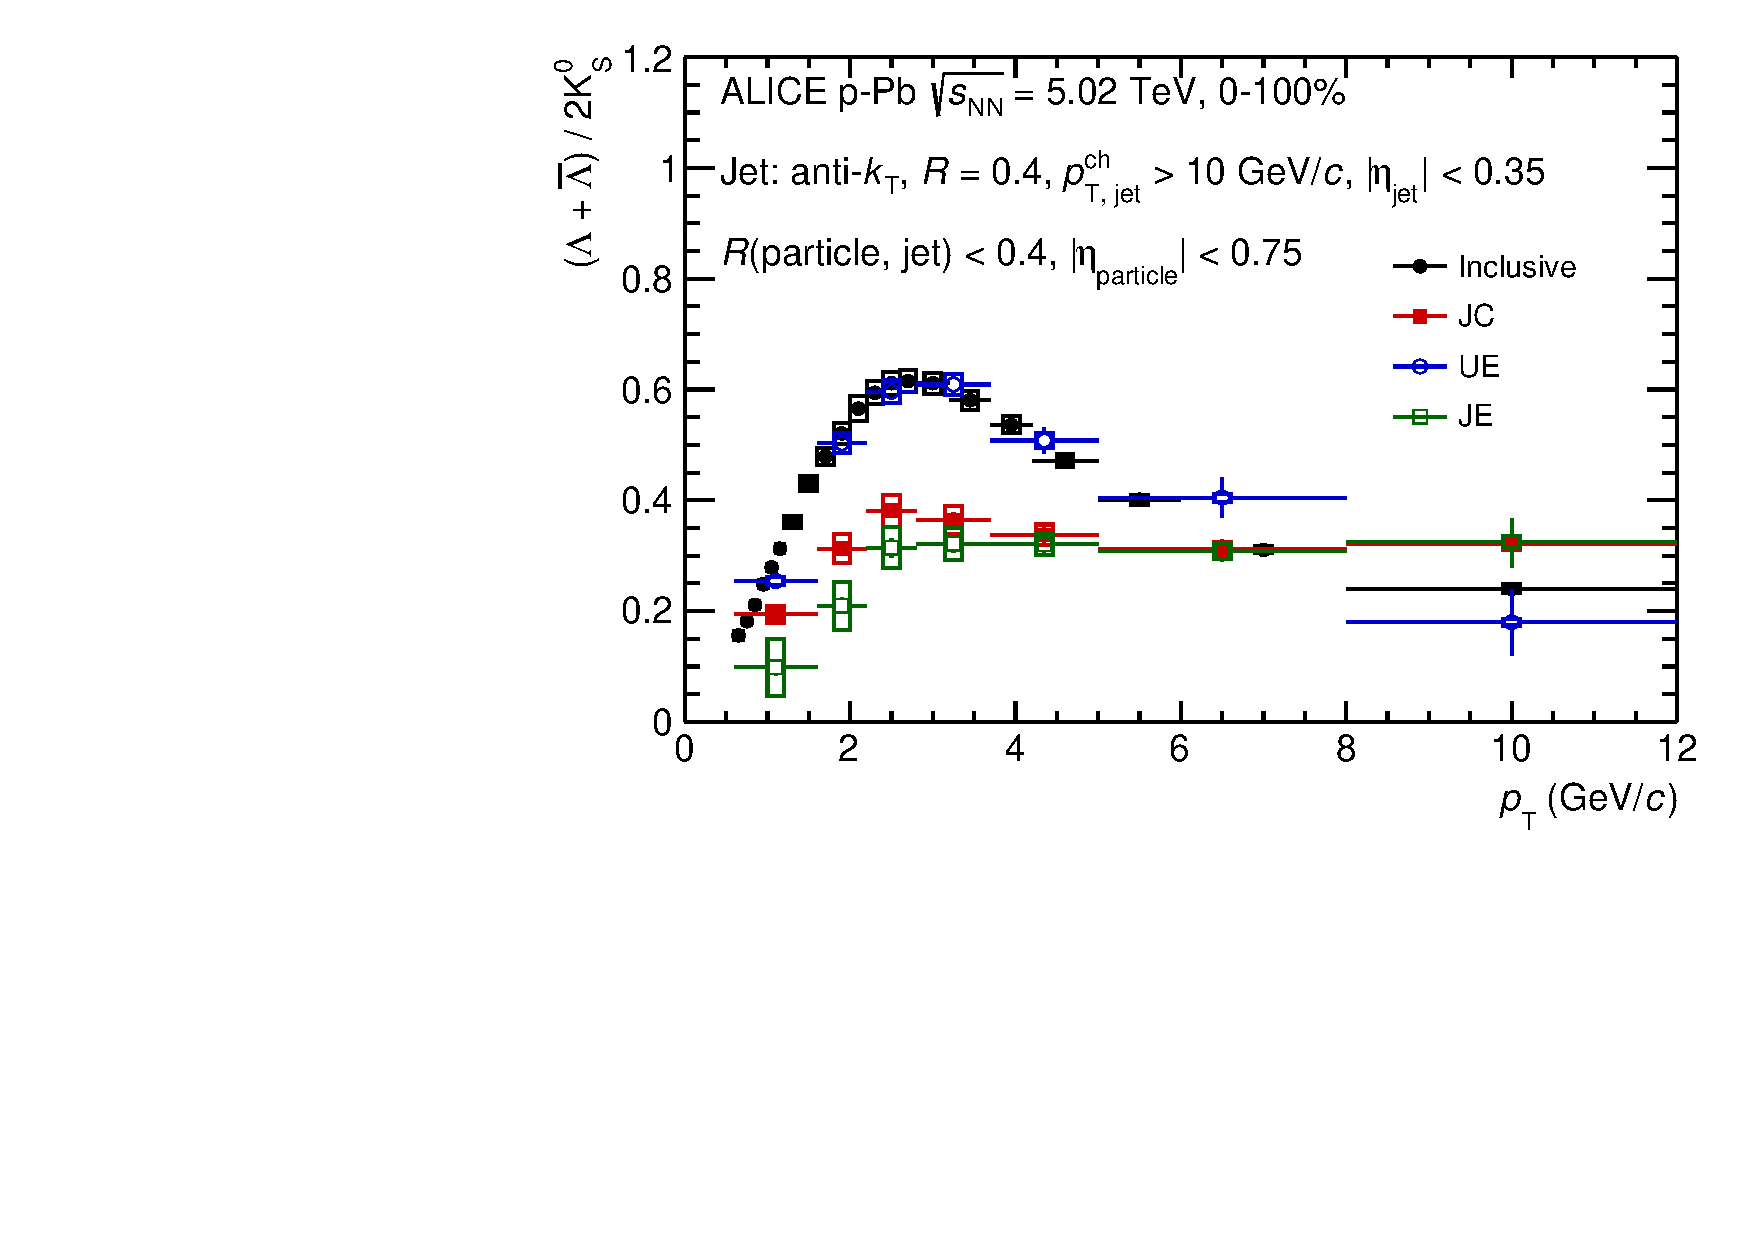
\includegraphics[width=.3\textwidth]{cf8_1}
		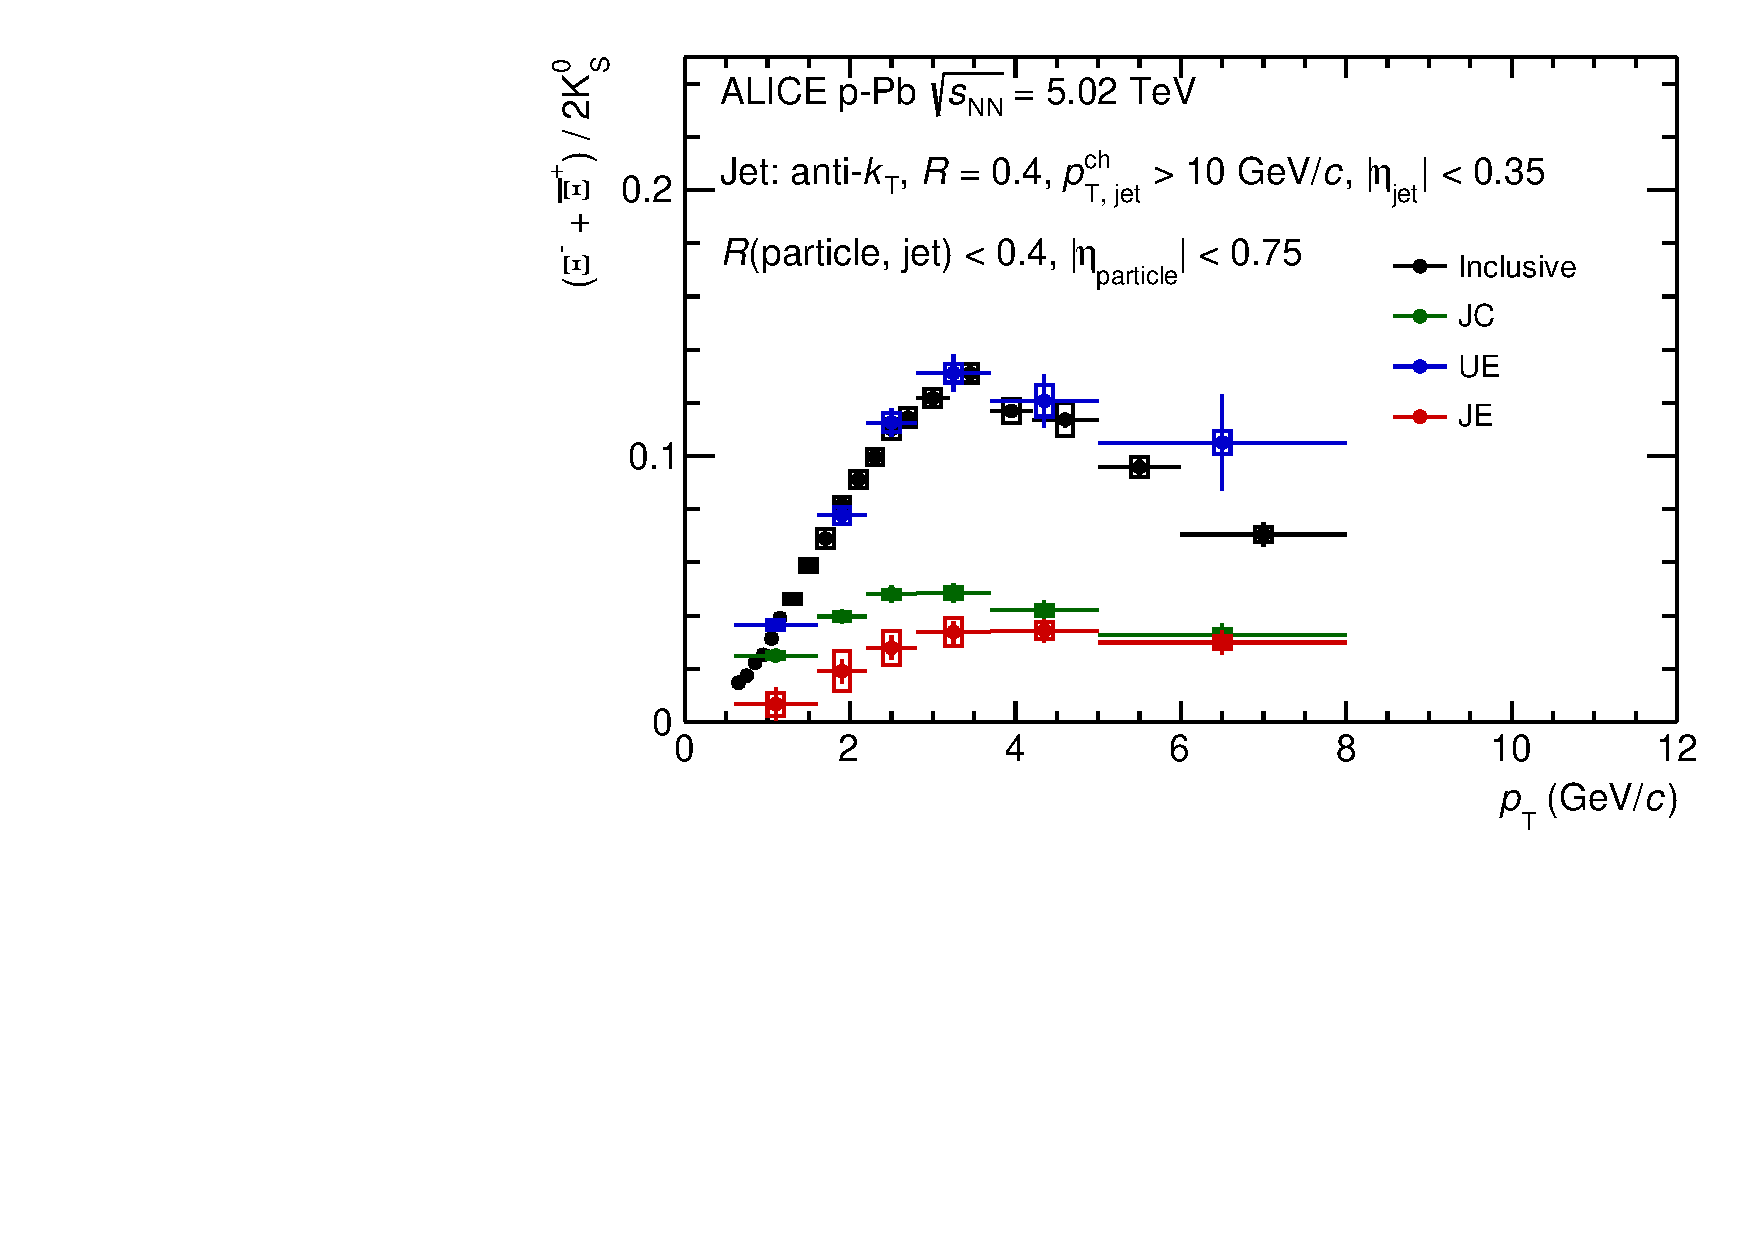
\includegraphics[width=.3\textwidth]{cf8_2}
		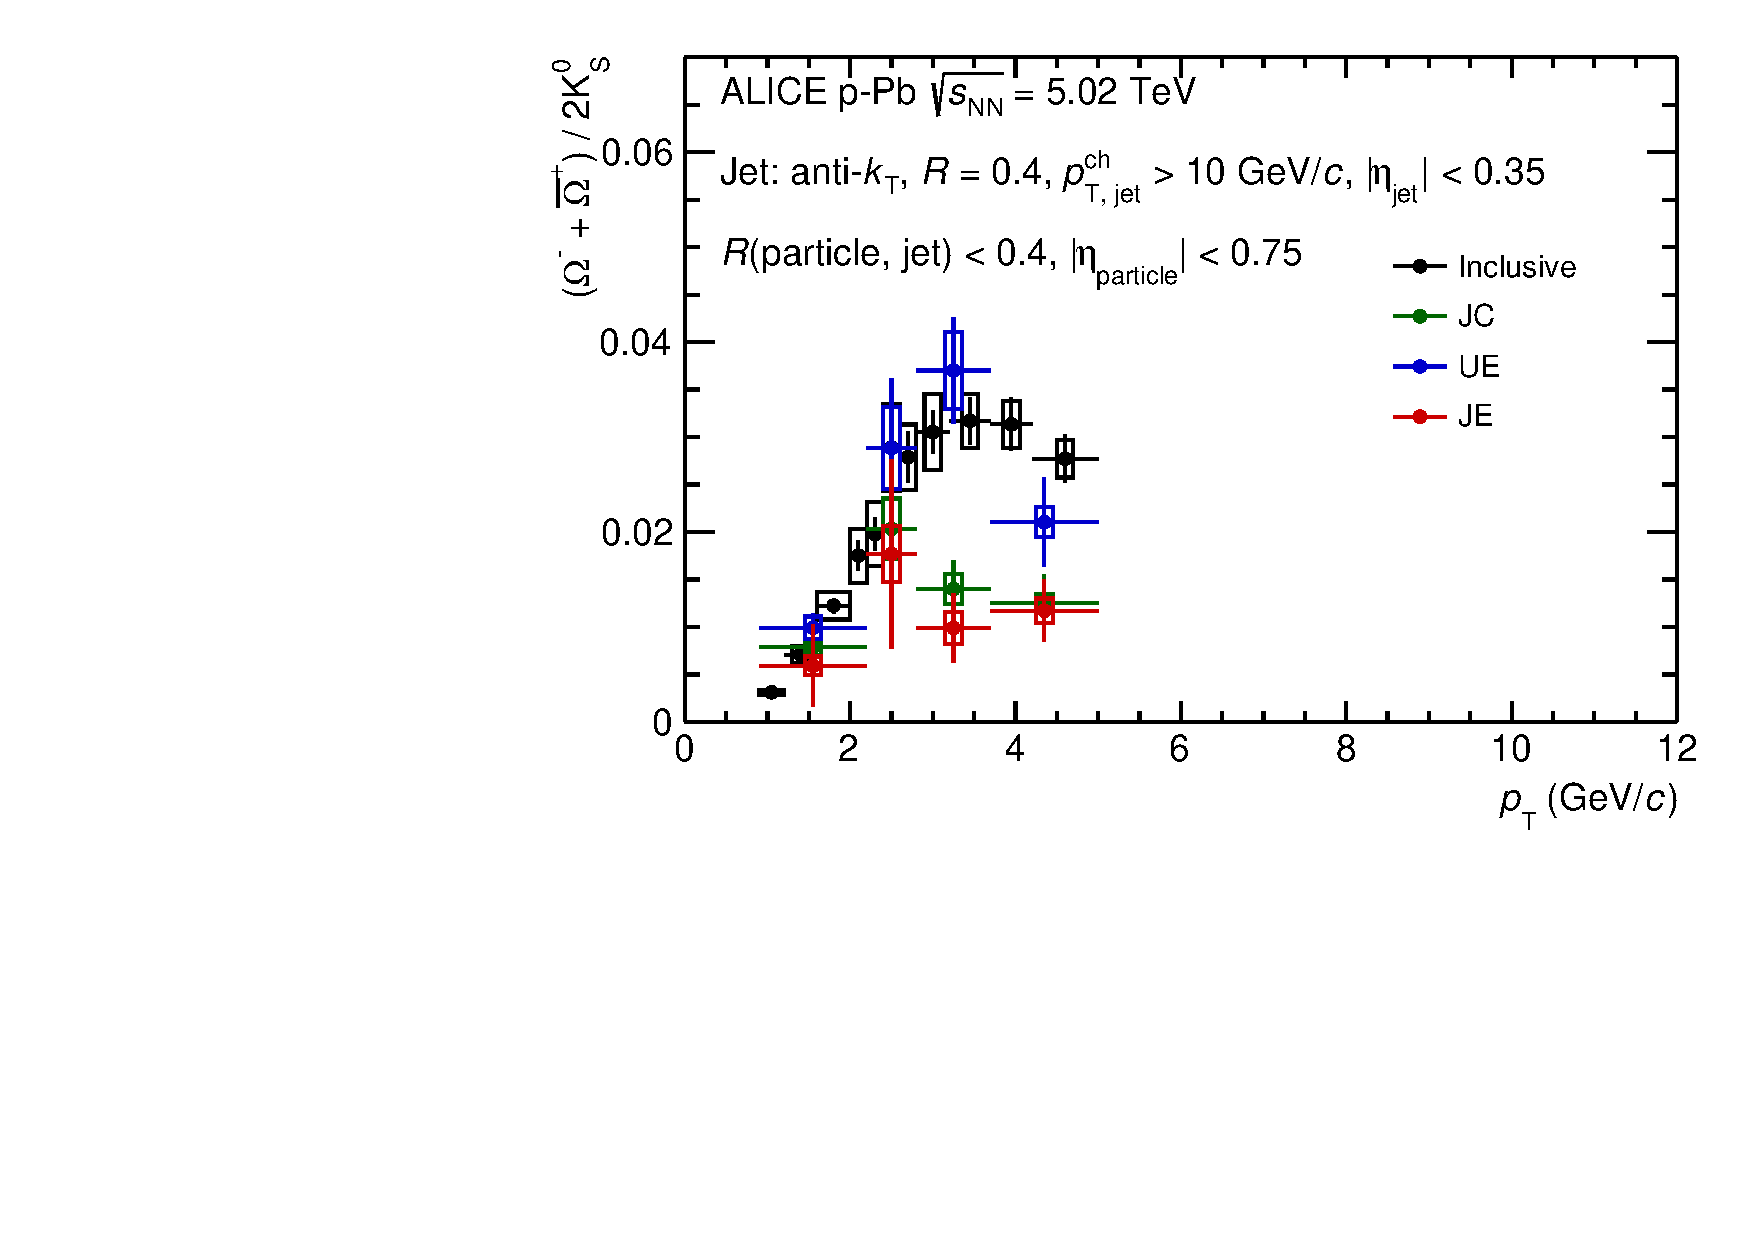
\includegraphics[width=.3\textwidth]{cf8_3}
		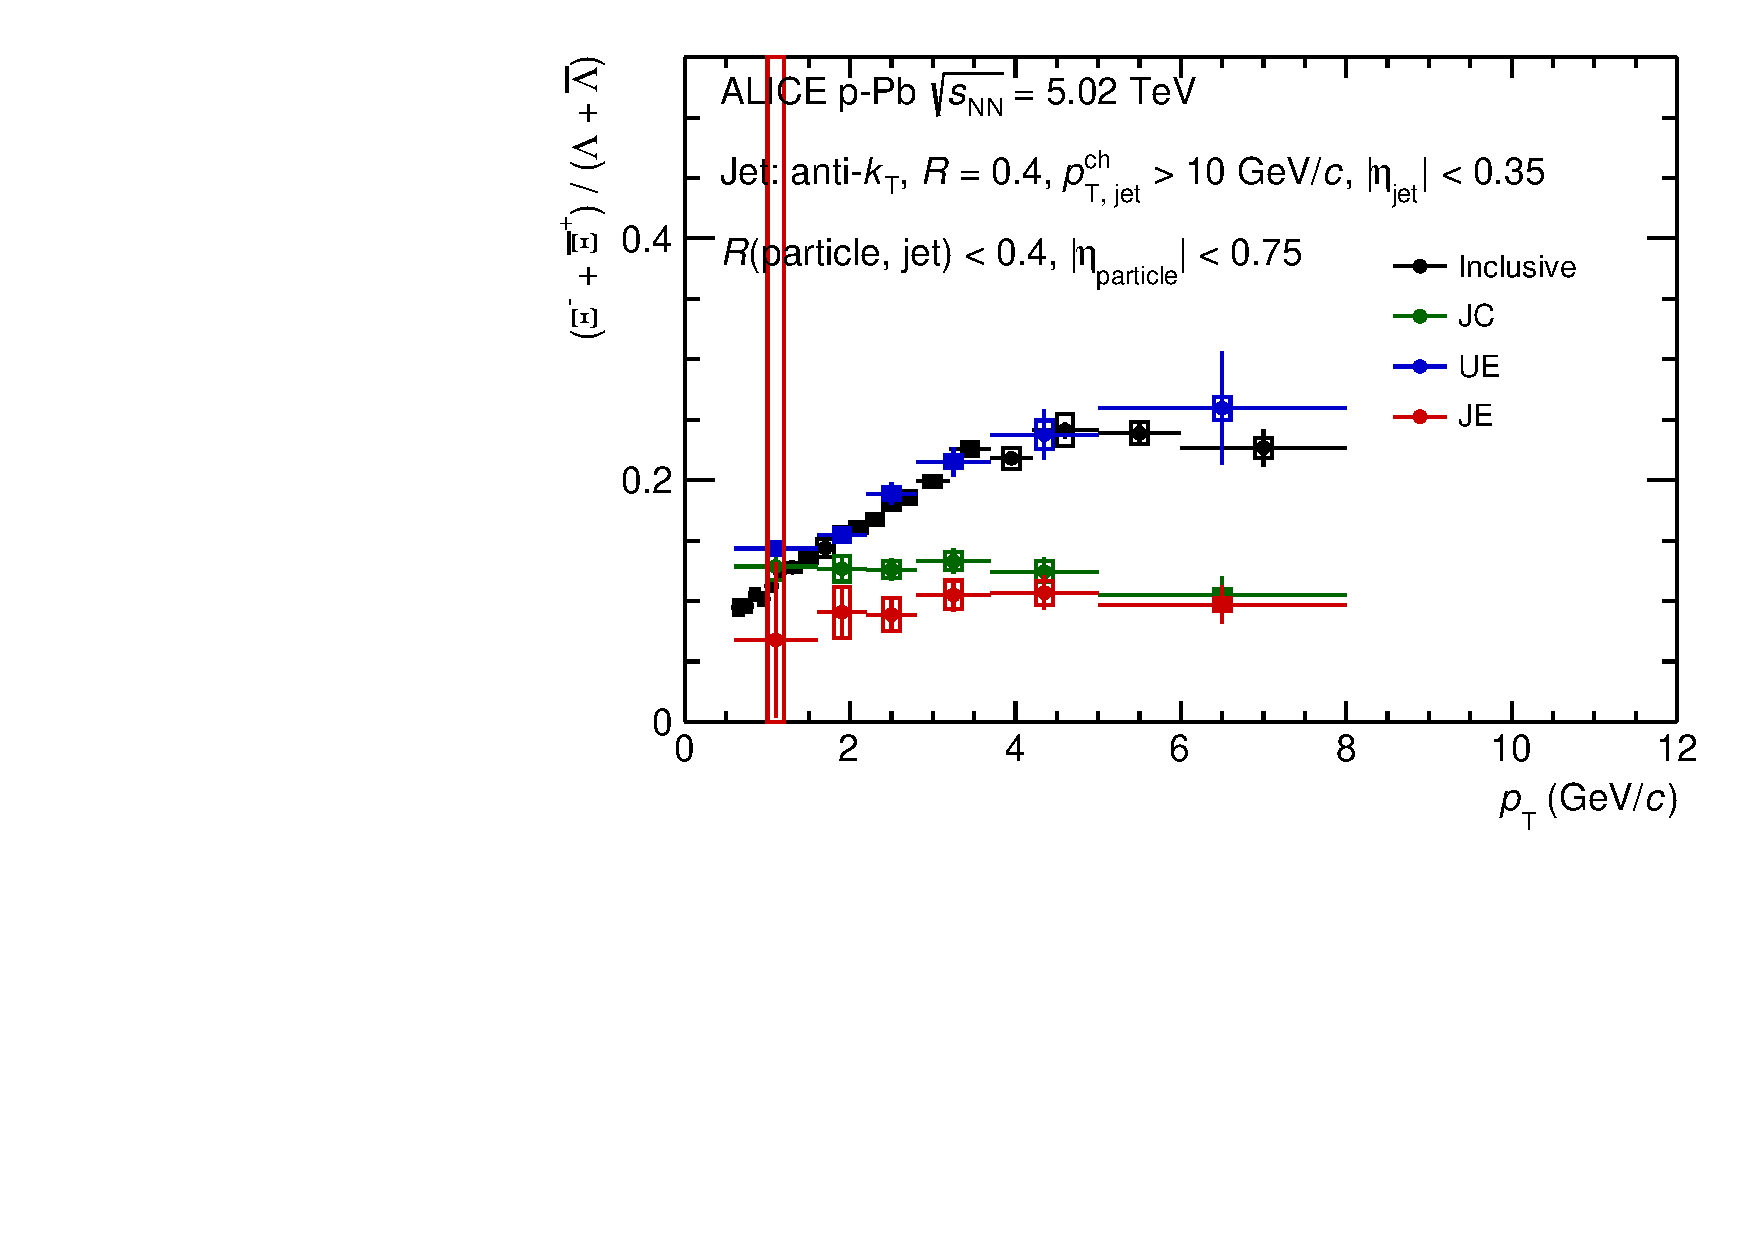
\includegraphics[width=.3\textwidth]{cf8_4}
		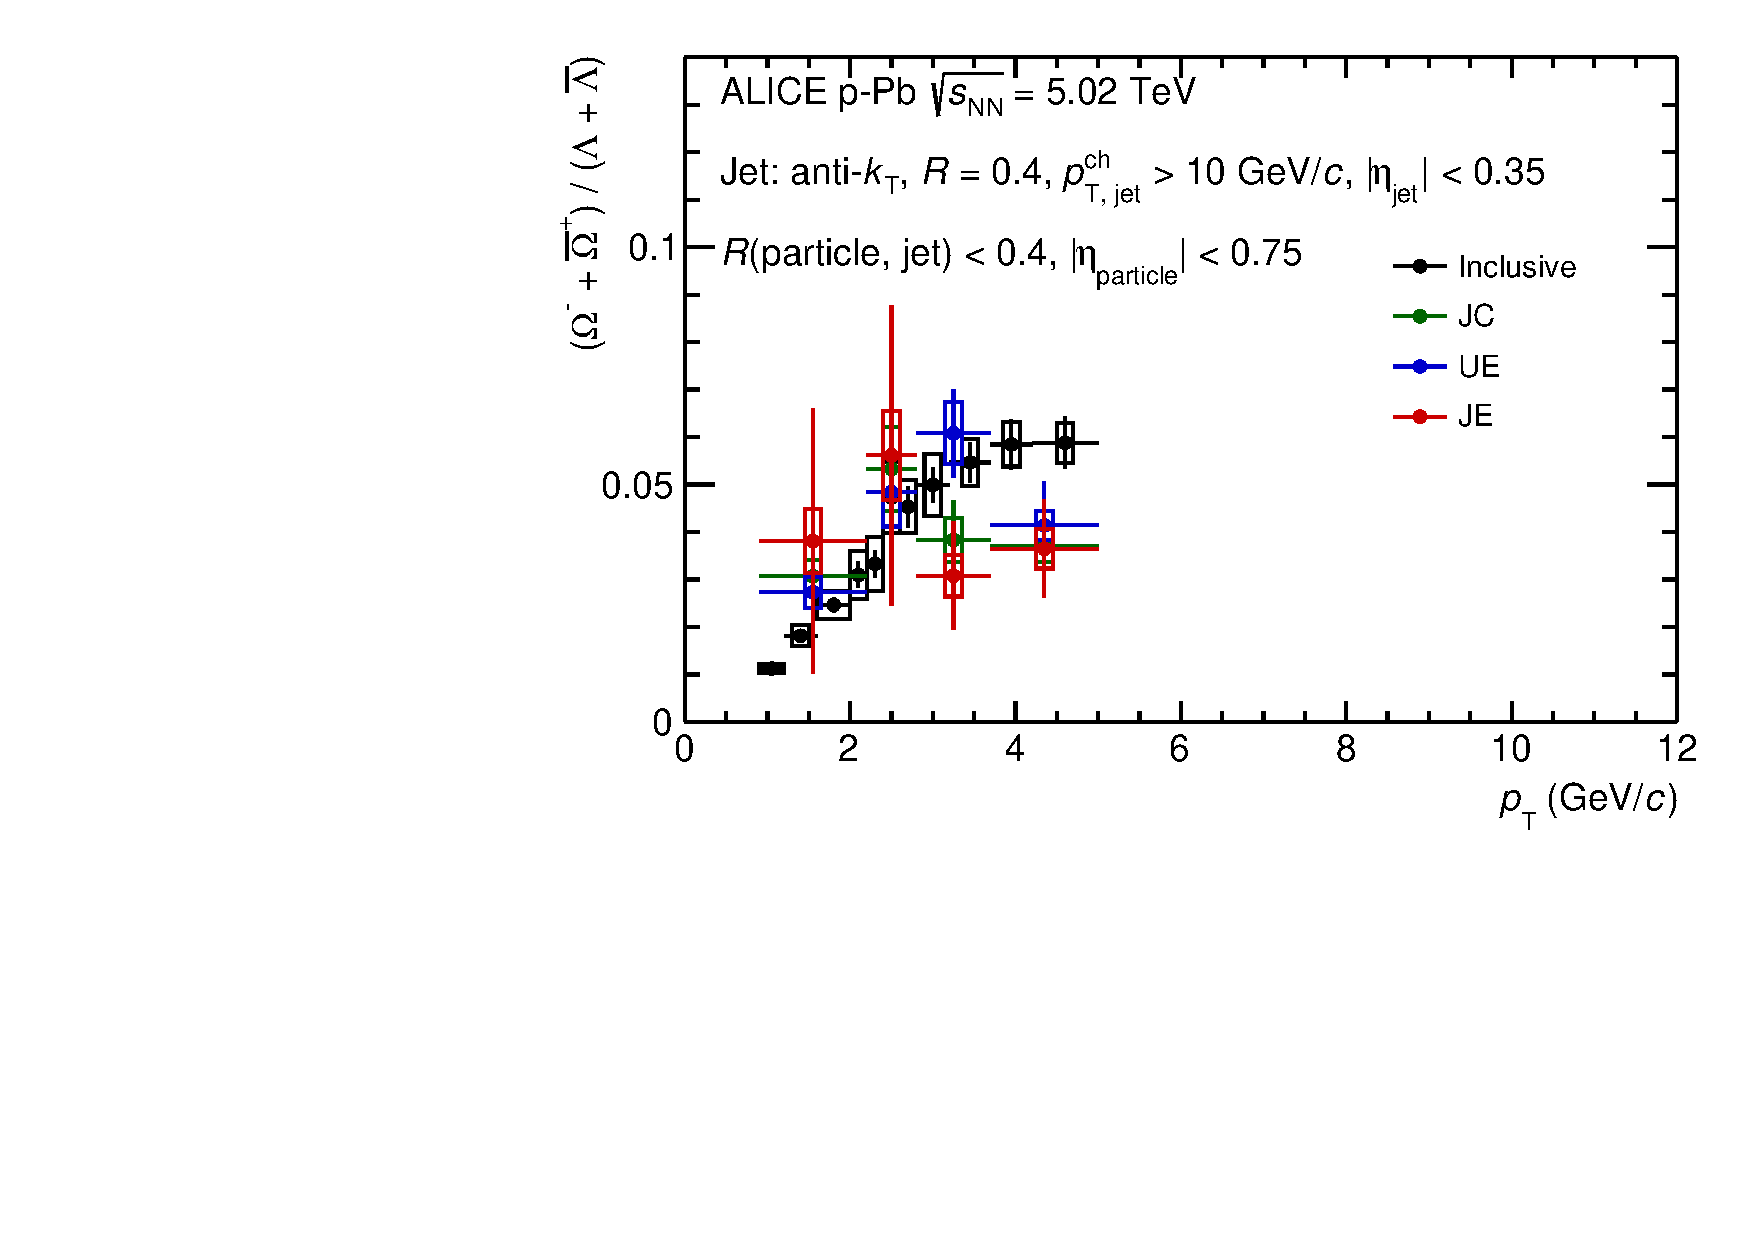
\includegraphics[width=.3\textwidth]{cf8_5}
		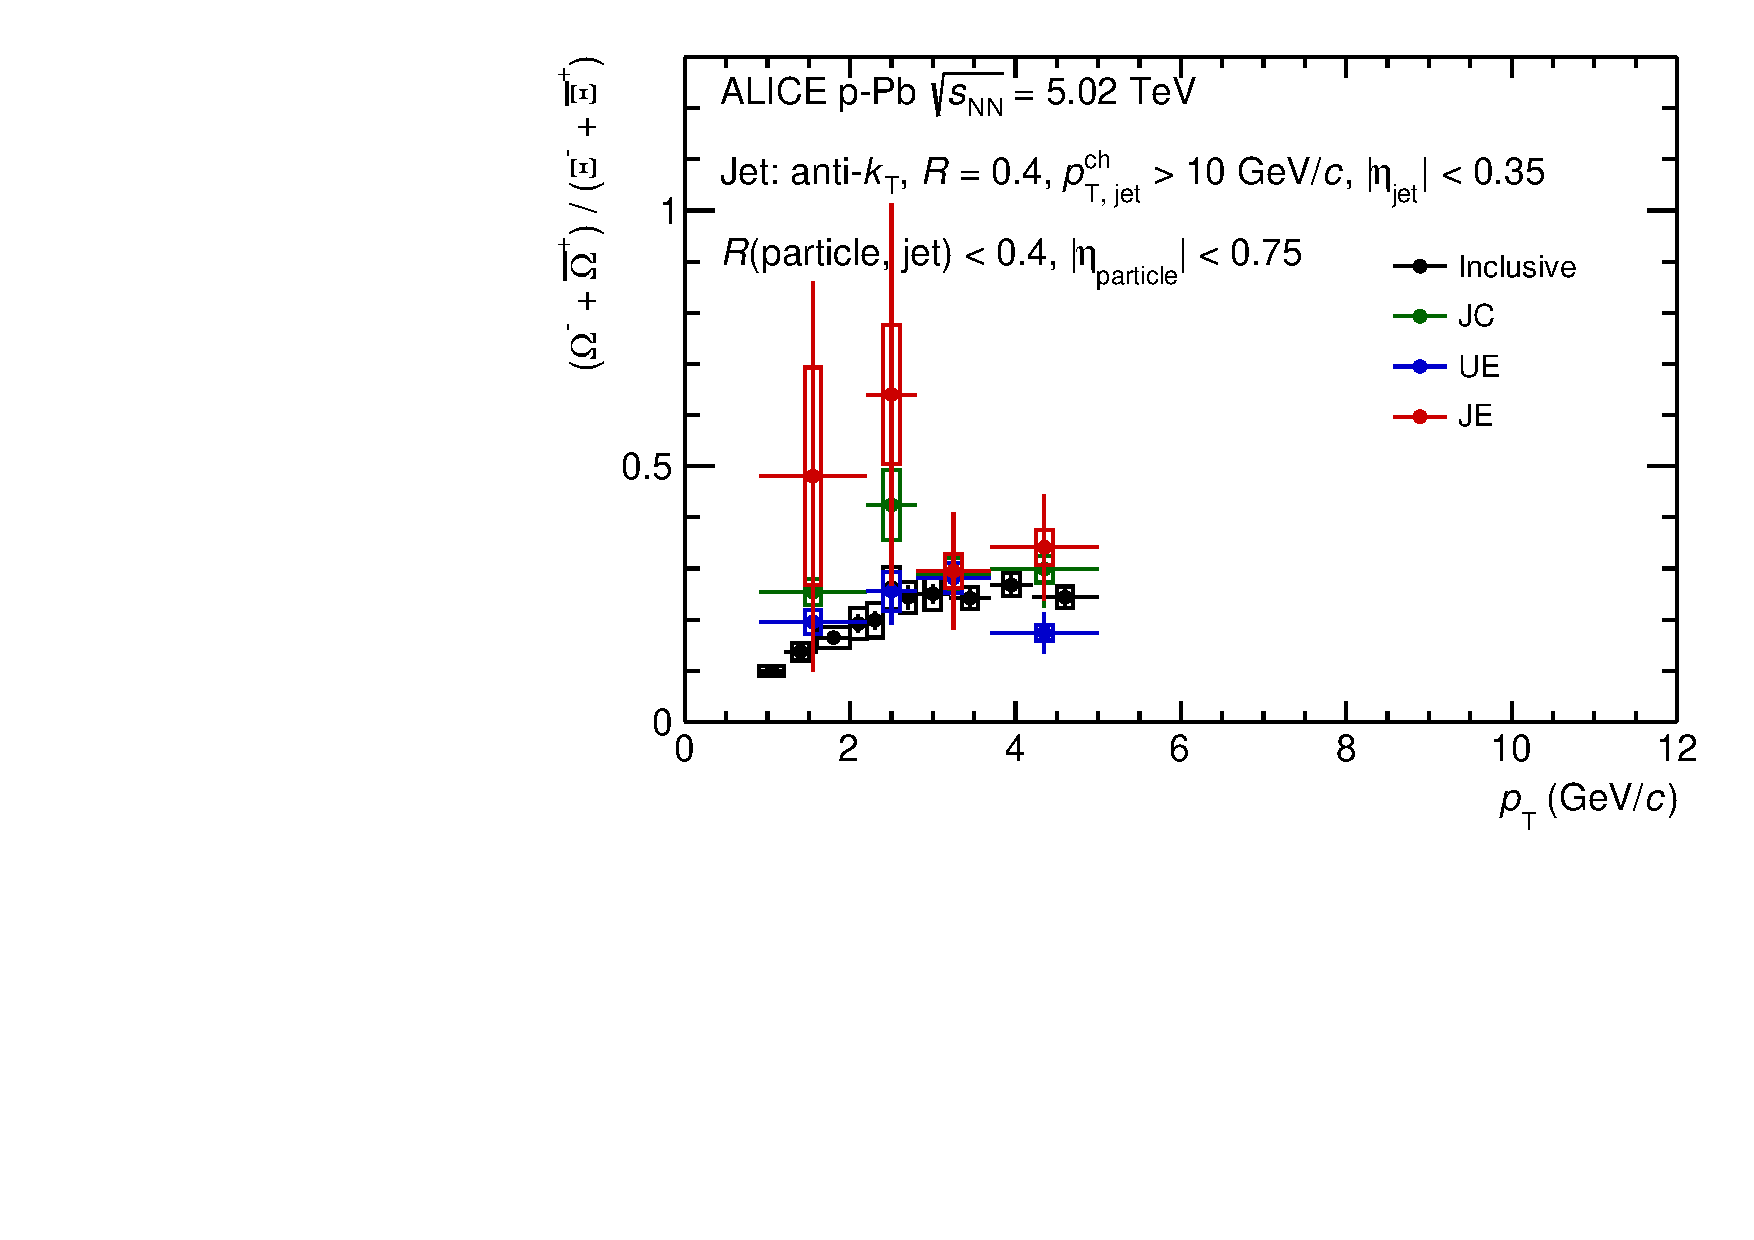
\includegraphics[width=.3\textwidth]{cf8_6}
	\end{center}
	\caption{Particle ratios in \pPb.}
	\label{fig:pPbRatio}
\end{figure}
\begin{figure}[!ht]
	\begin{center}
		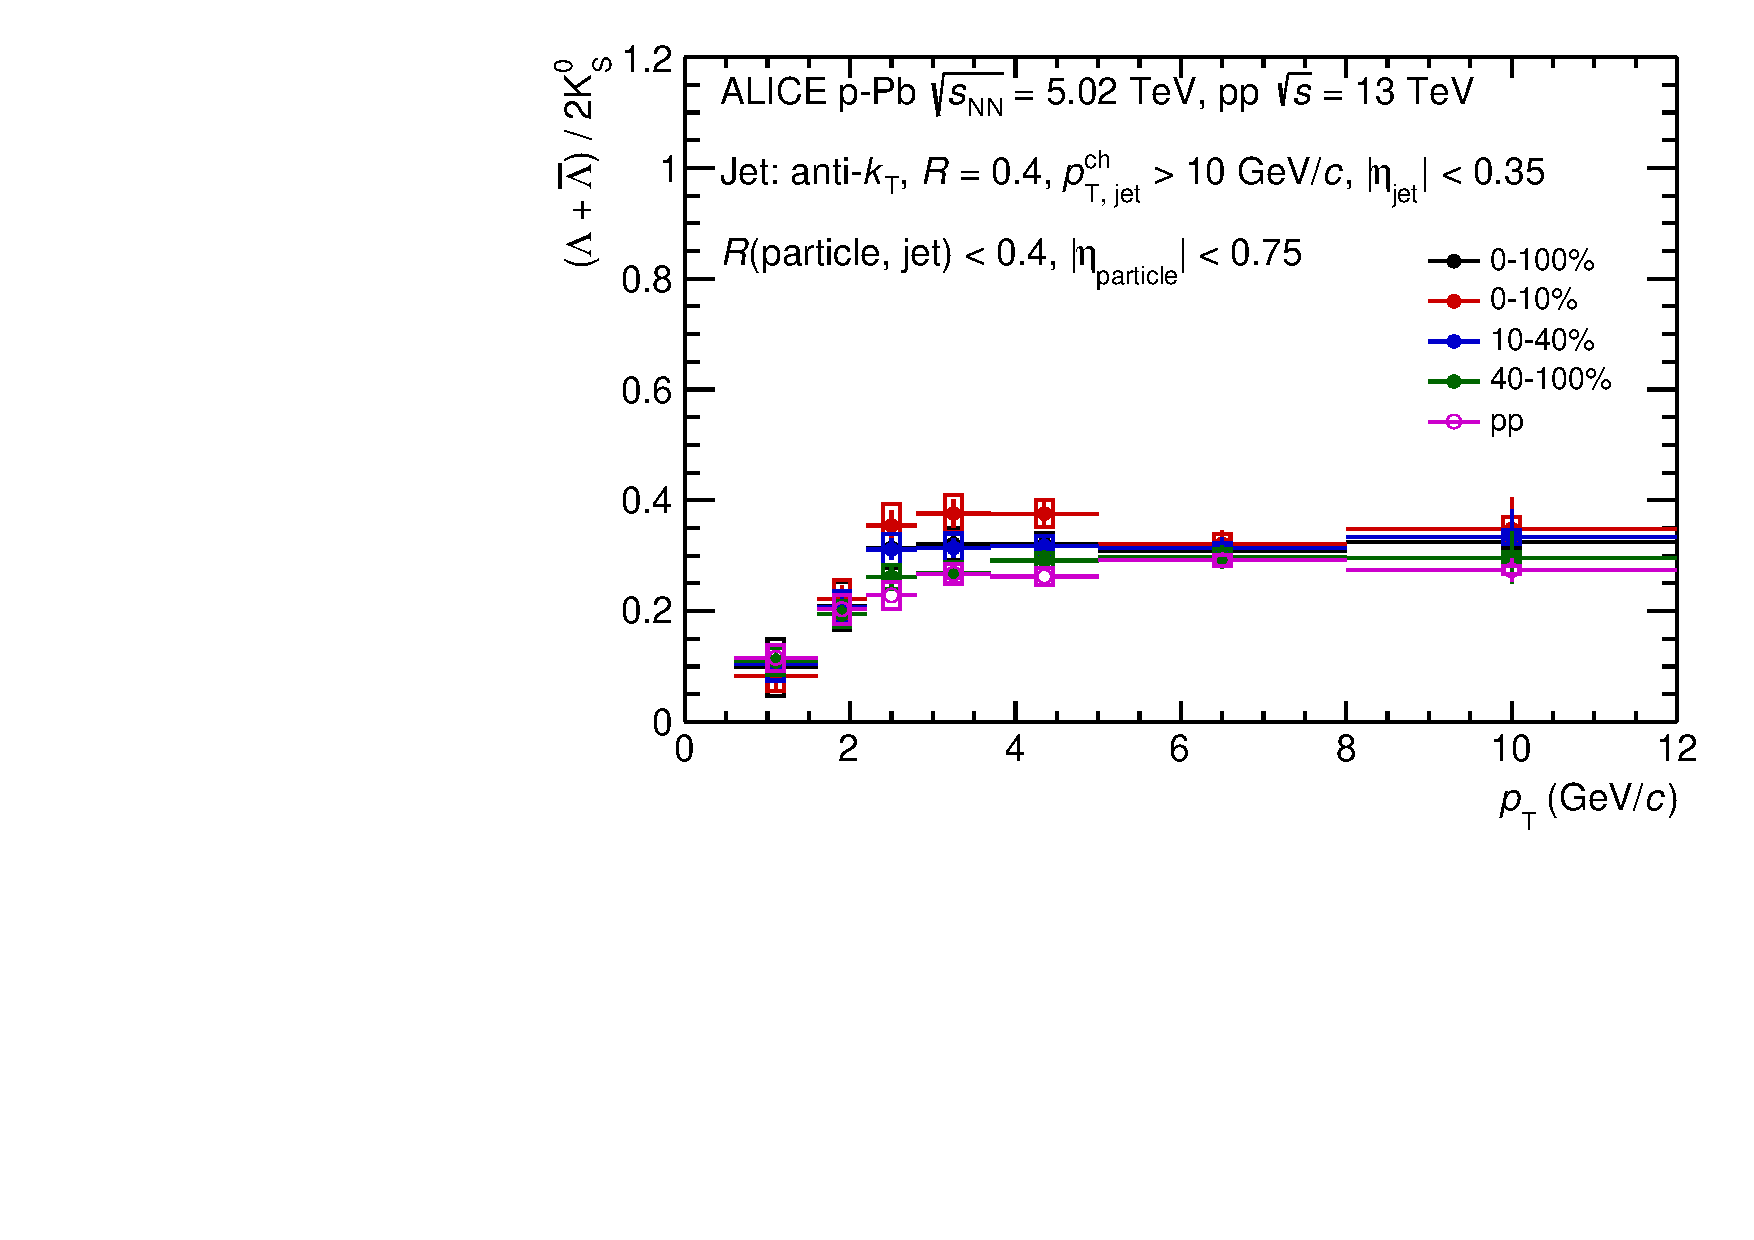
\includegraphics[width=.3\textwidth]{cf9_1}
		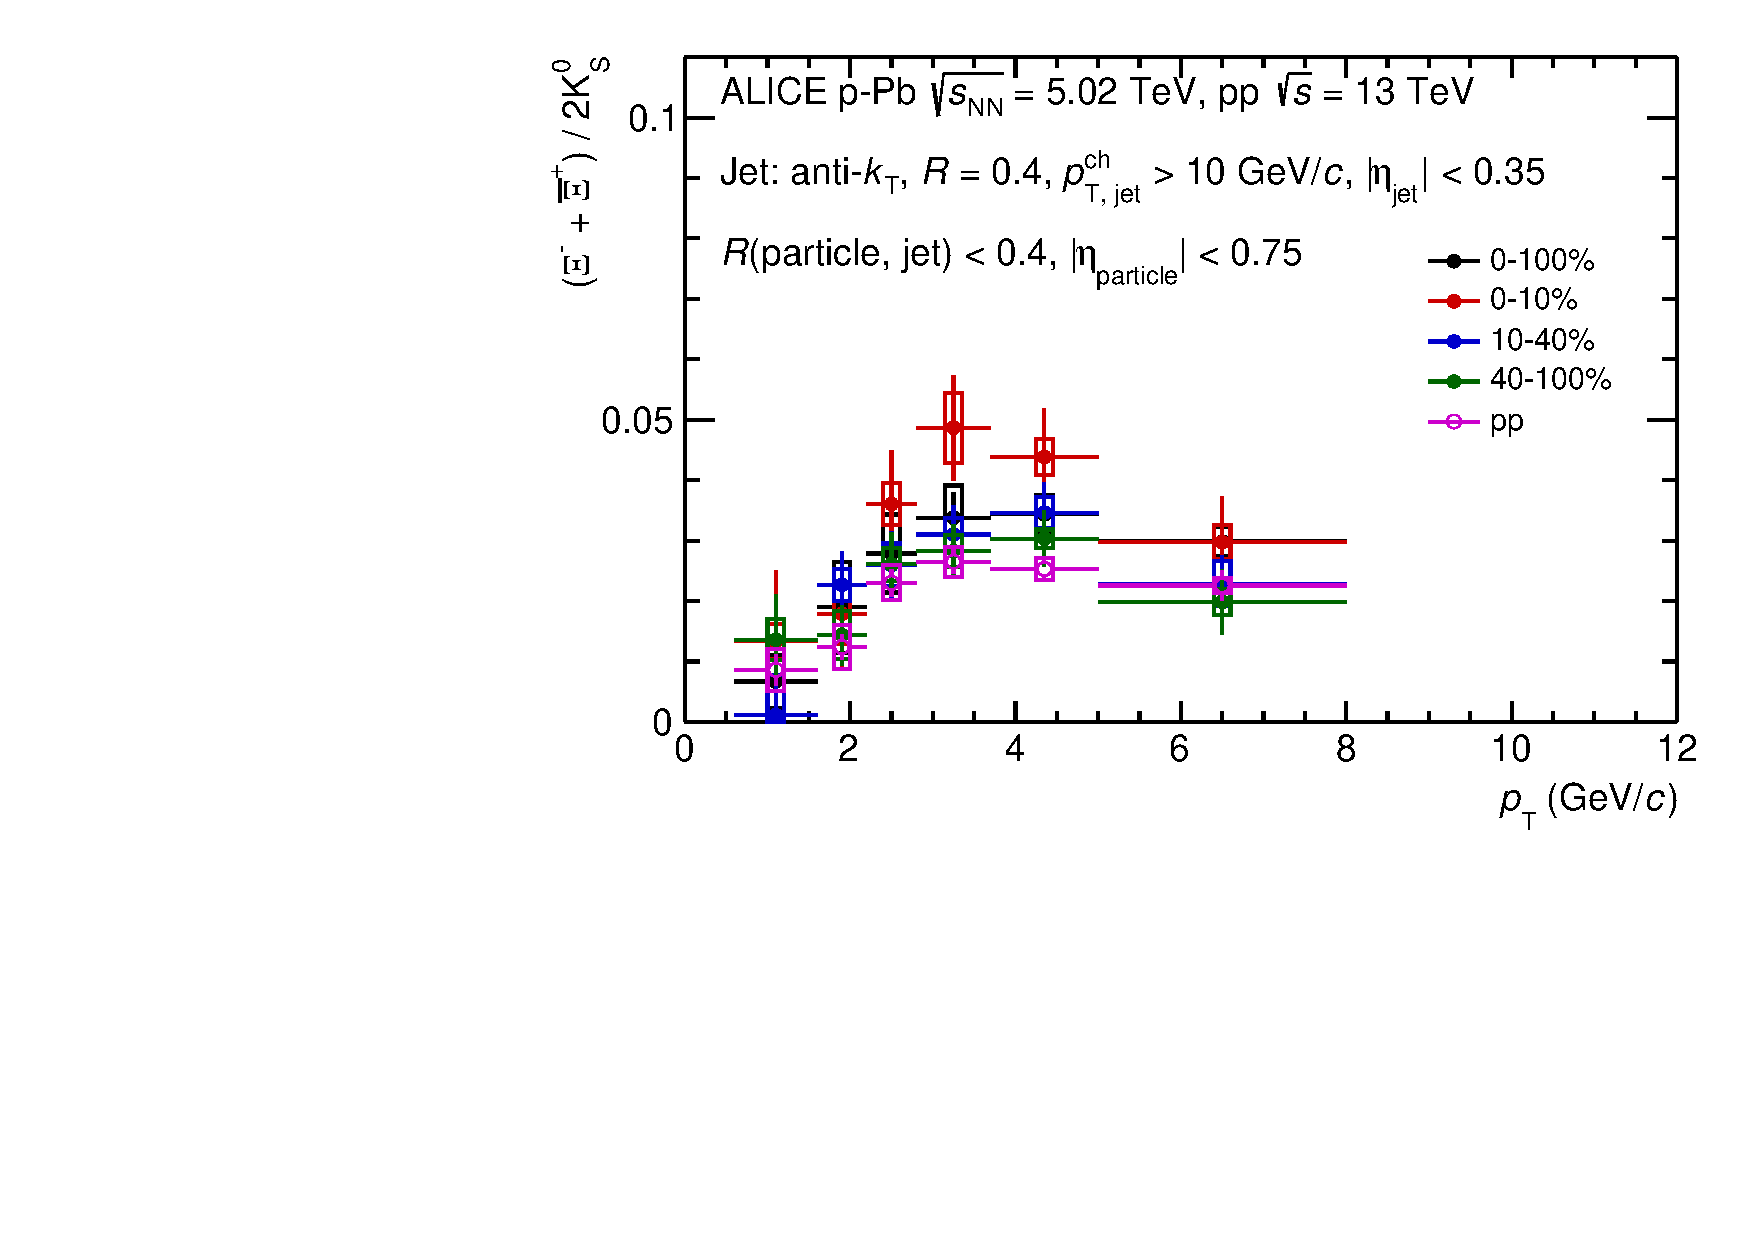
\includegraphics[width=.3\textwidth]{cf9_2}
		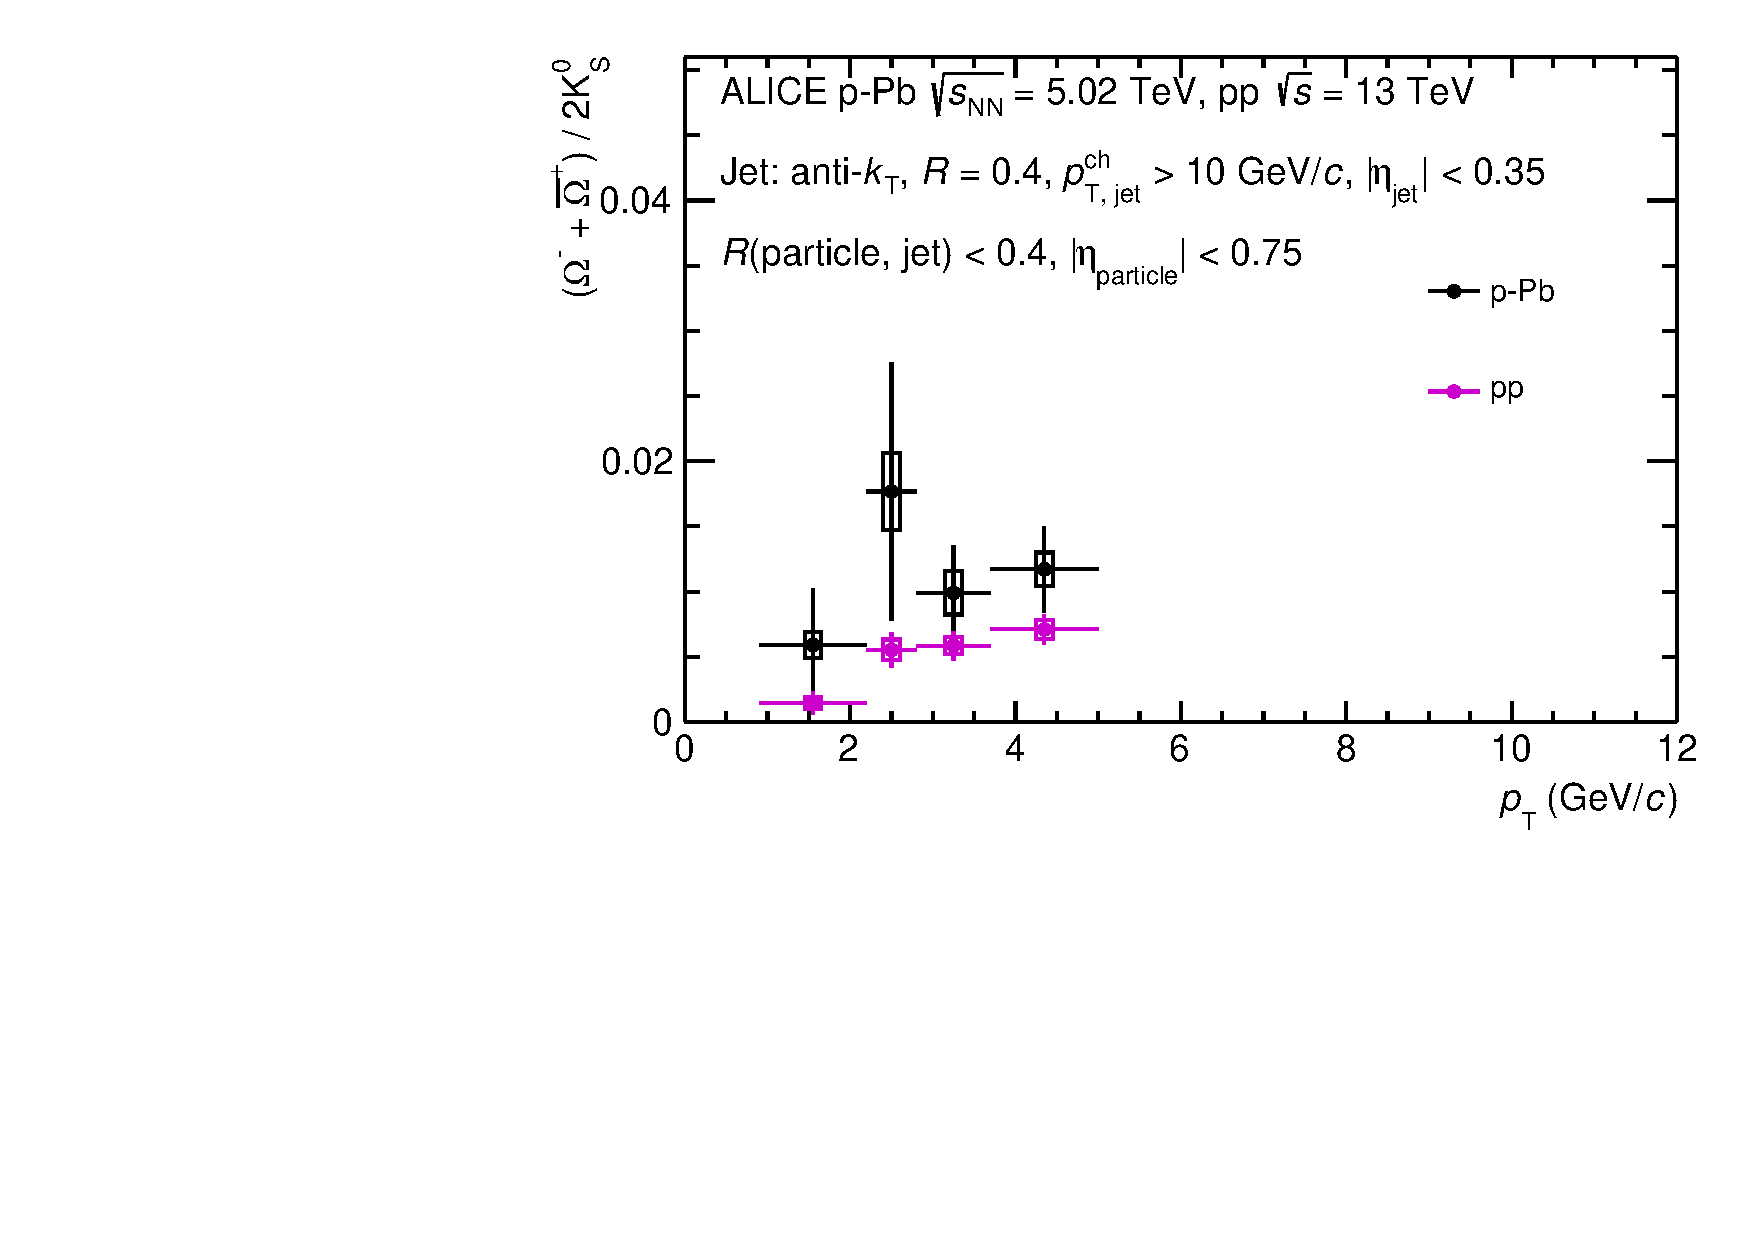
\includegraphics[width=.3\textwidth]{cf9_3}
		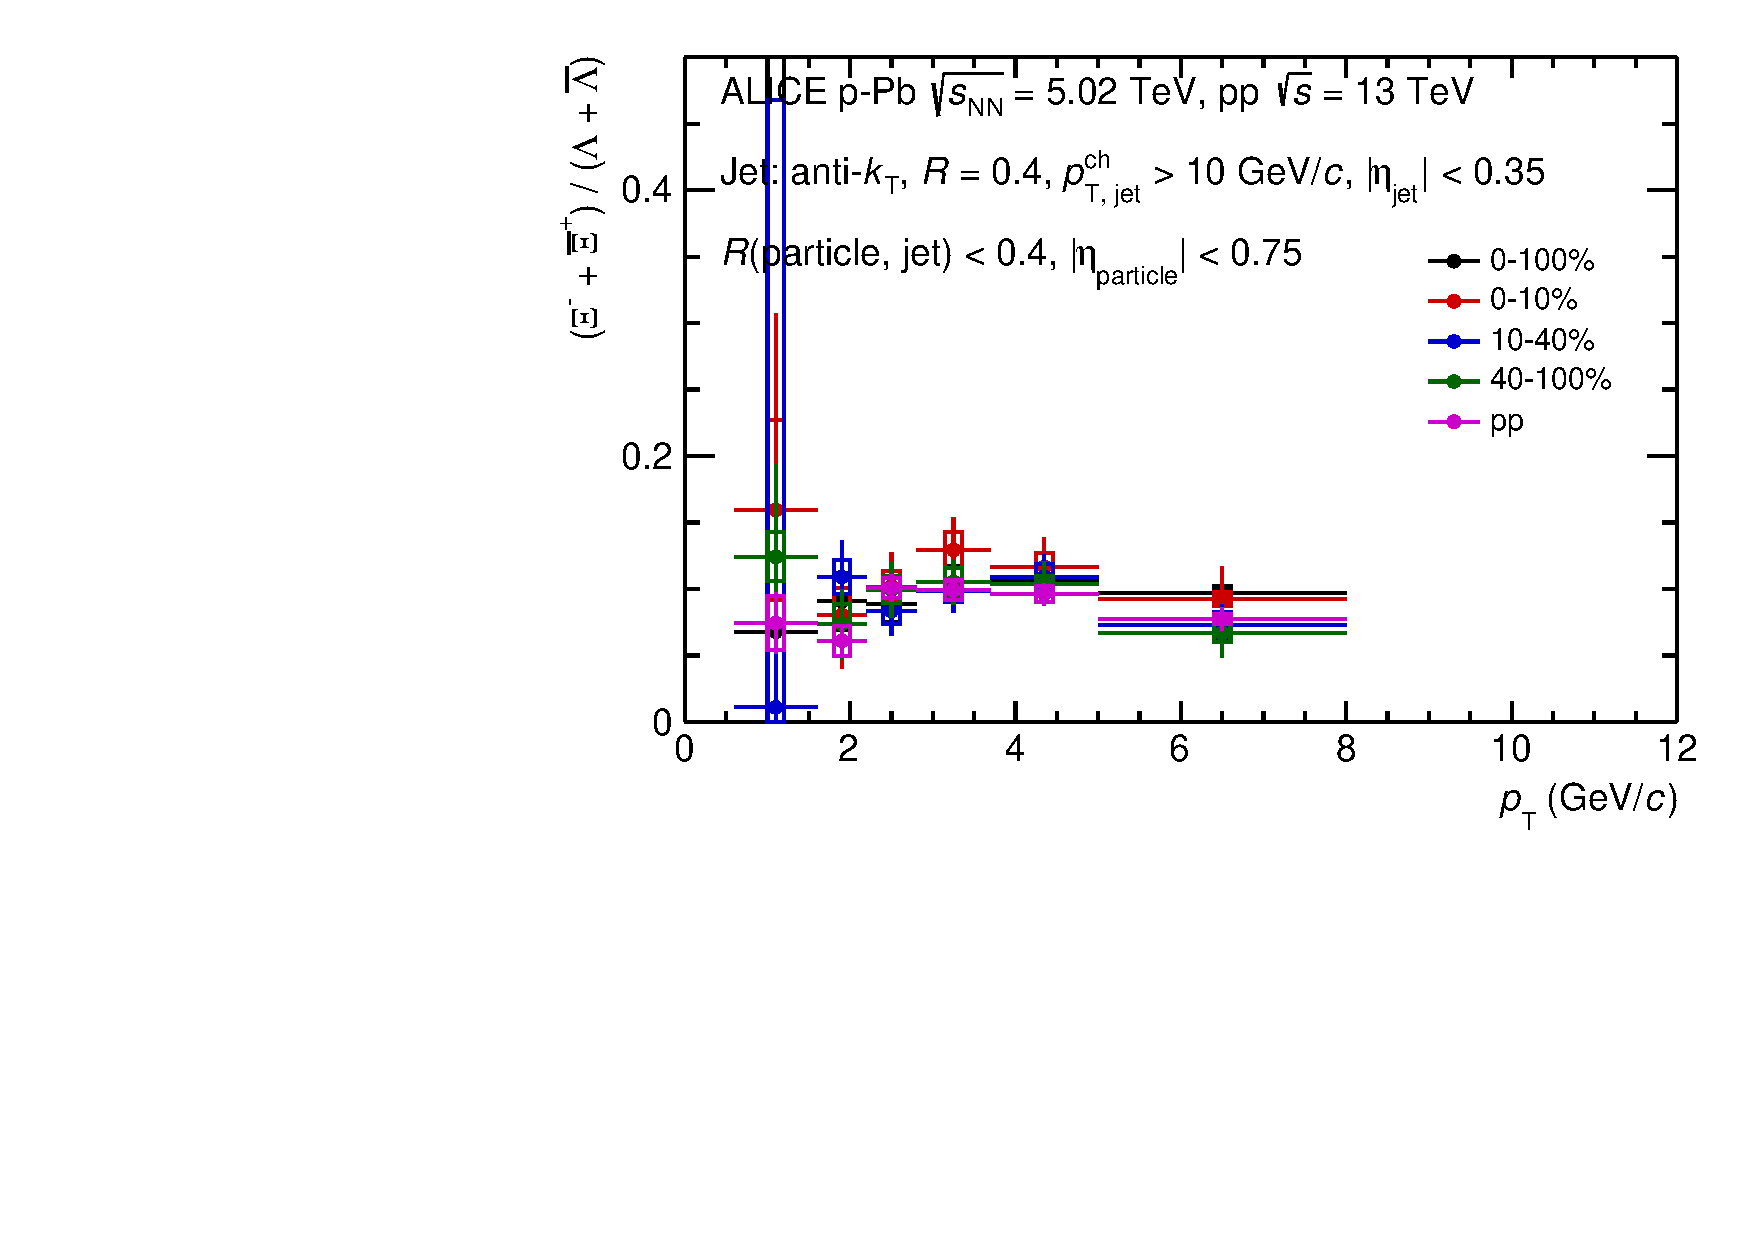
\includegraphics[width=.3\textwidth]{cf9_4}
		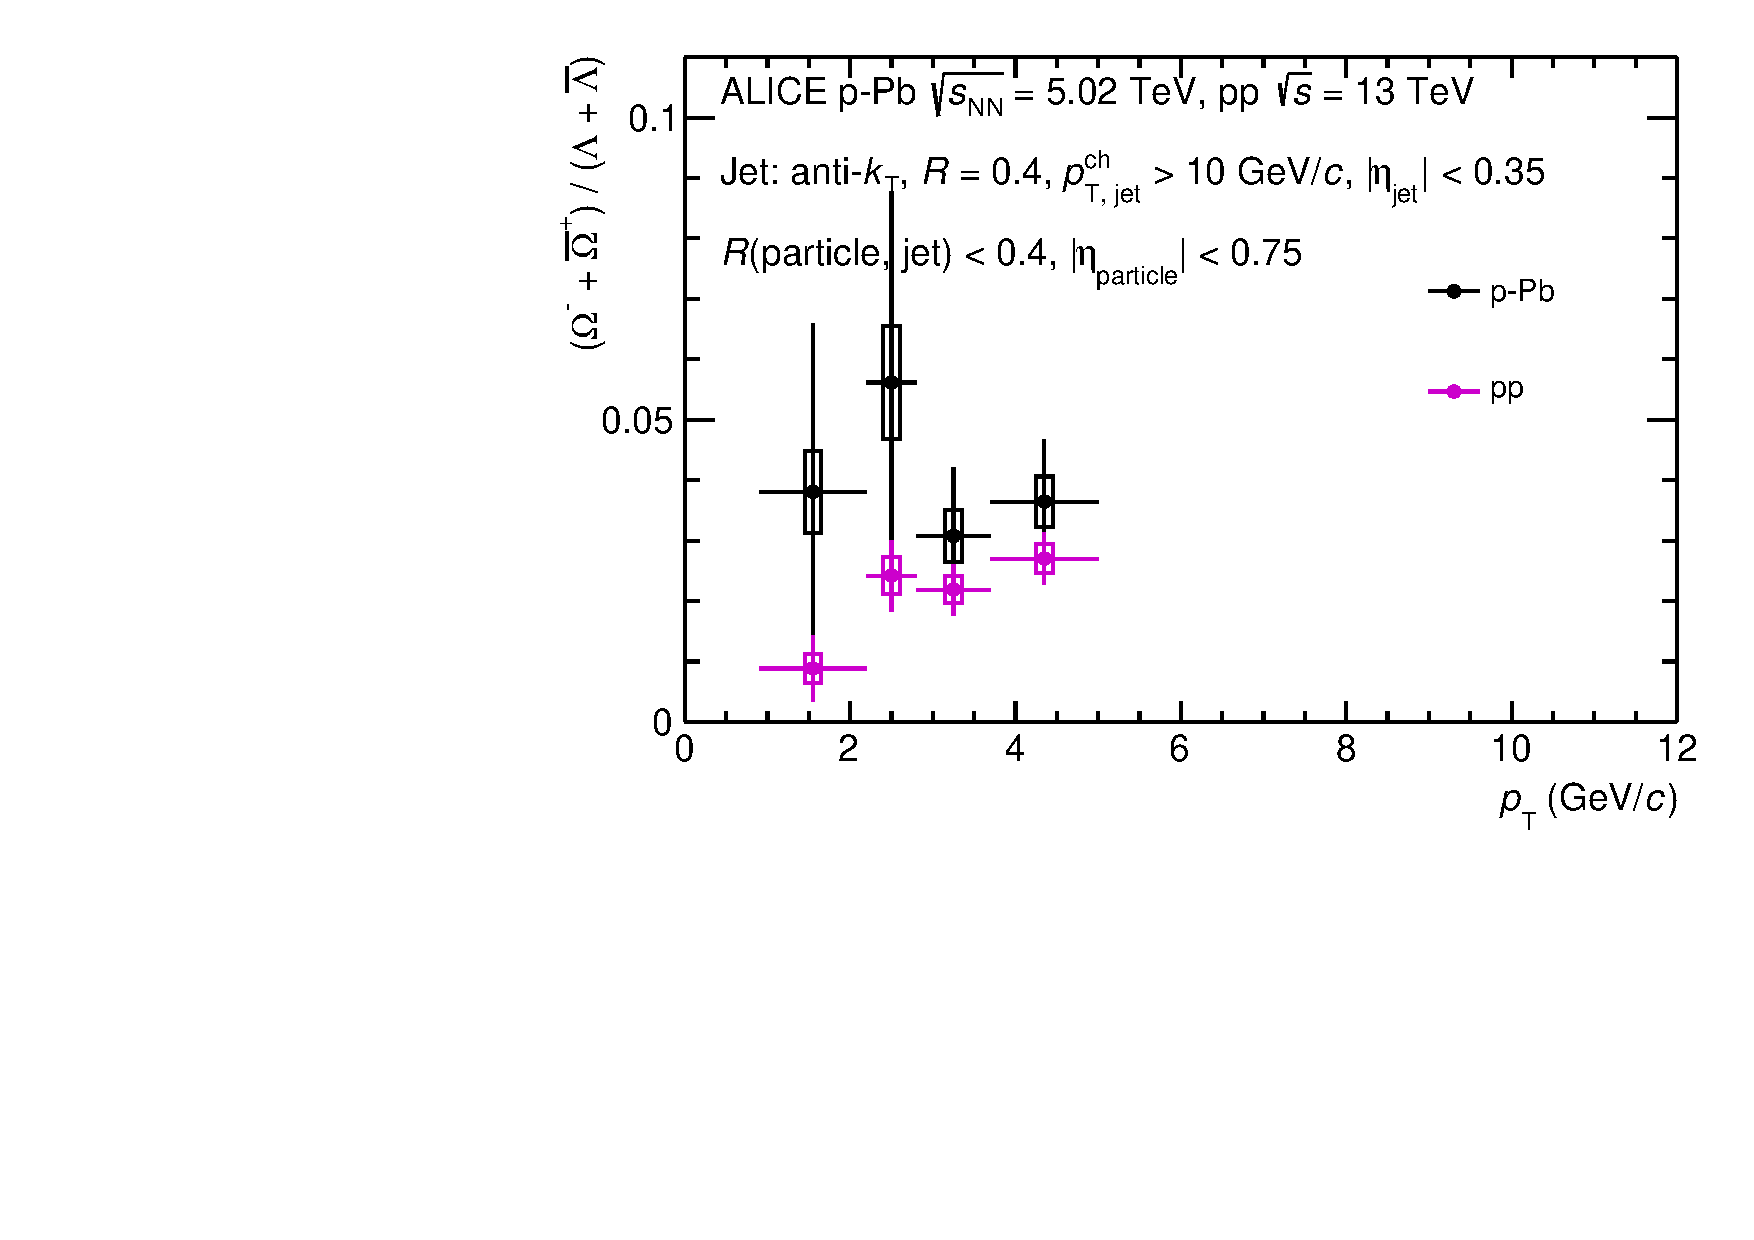
\includegraphics[width=.3\textwidth]{cf9_5}
		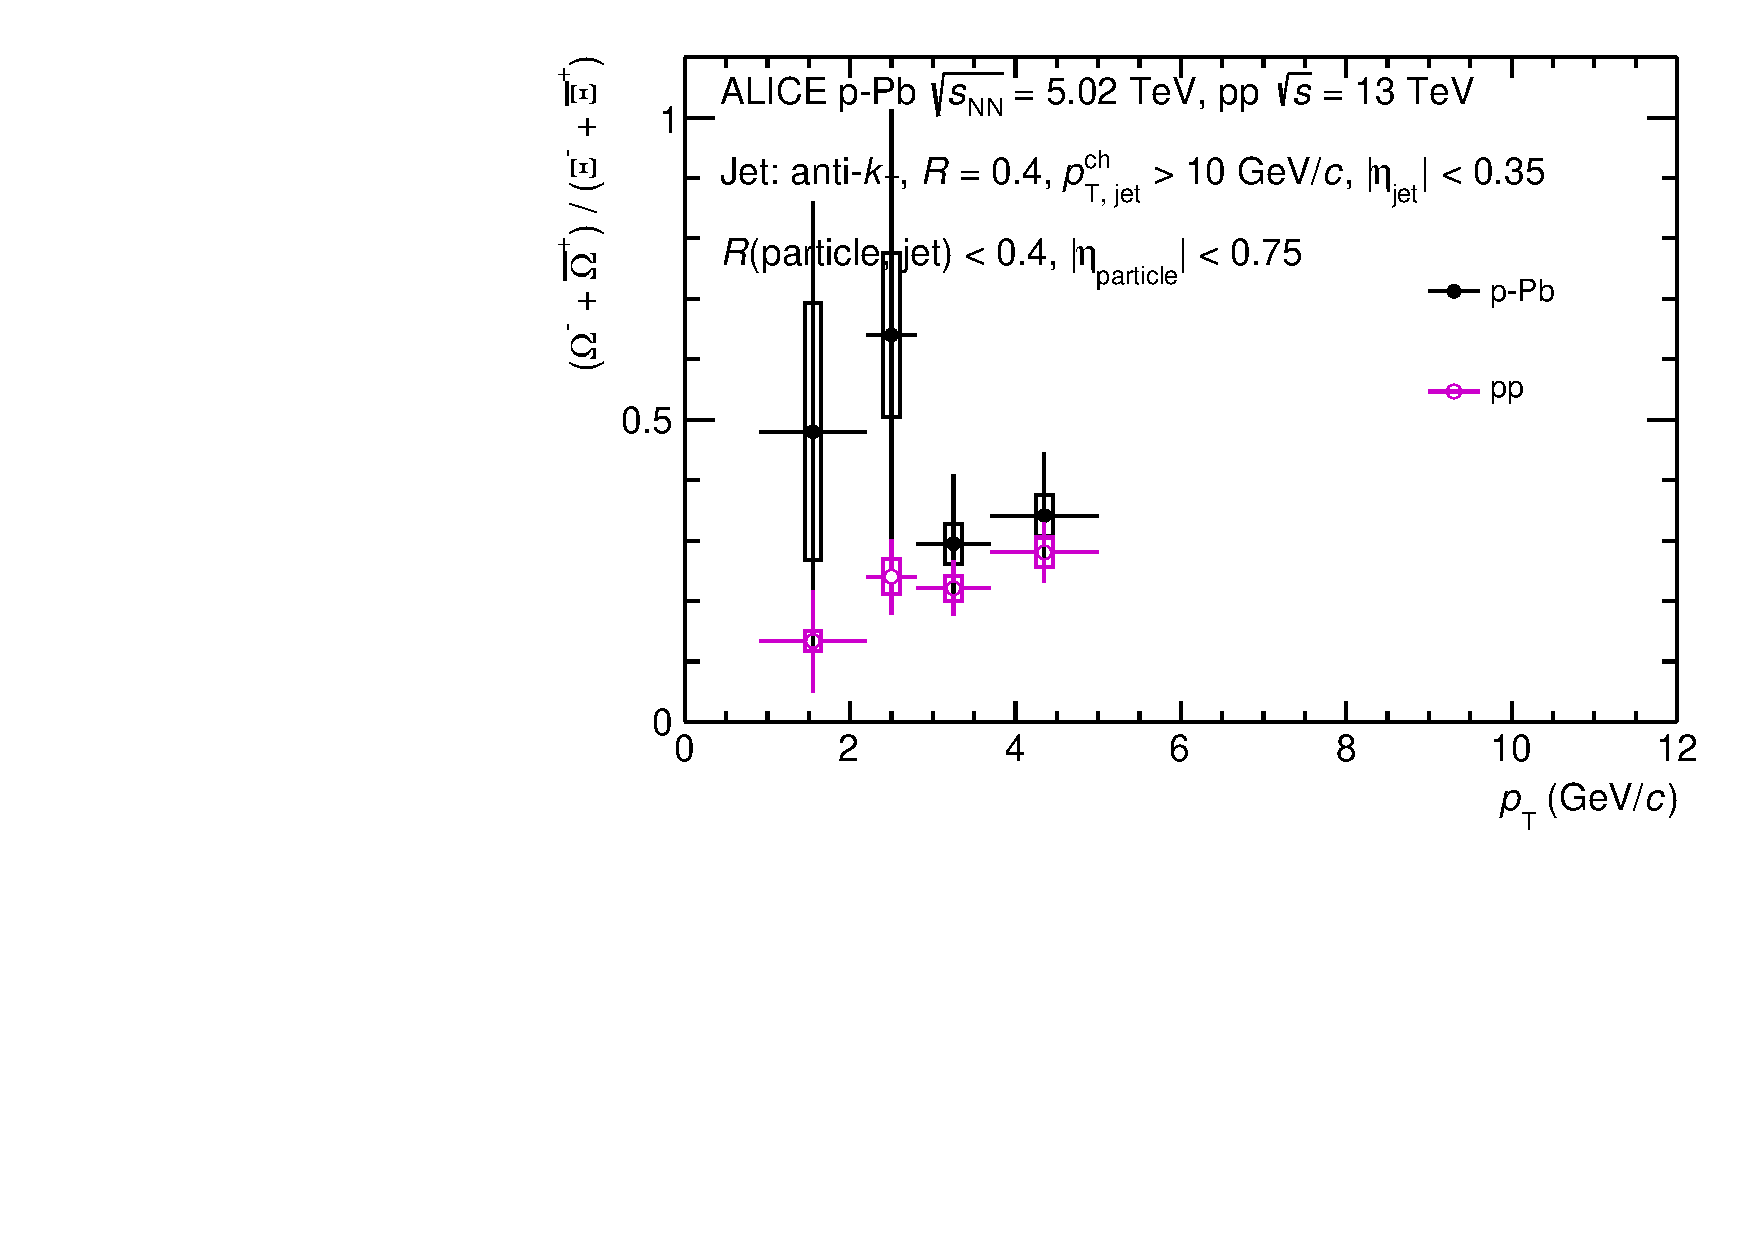
\includegraphics[width=.3\textwidth]{cf9_6}
	\end{center}
	\caption{Particle ratios.}
	\label{fig:pppPbRatio}
\end{figure}

\subsection{Compare to models}
\label{subsec:ComToMod}
